\documentclass[twoside]{book}

% Packages required by doxygen
\usepackage{fixltx2e}
\usepackage{calc}
\usepackage{doxygen}
\usepackage[export]{adjustbox} % also loads graphicx
\usepackage{graphicx}
\usepackage[utf8]{inputenc}
\usepackage{makeidx}
\usepackage{multicol}
\usepackage{multirow}
\PassOptionsToPackage{warn}{textcomp}
\usepackage{textcomp}
\usepackage[nointegrals]{wasysym}
\usepackage[table]{xcolor}

% Font selection
\usepackage[T1]{fontenc}
\usepackage[scaled=.90]{helvet}
\usepackage{courier}
\usepackage{amssymb}
\usepackage{sectsty}
\renewcommand{\familydefault}{\sfdefault}
\allsectionsfont{%
  \fontseries{bc}\selectfont%
  \color{darkgray}%
}
\renewcommand{\DoxyLabelFont}{%
  \fontseries{bc}\selectfont%
  \color{darkgray}%
}
\newcommand{\+}{\discretionary{\mbox{\scriptsize$\hookleftarrow$}}{}{}}

% Page & text layout
\usepackage{geometry}
\geometry{%
  a4paper,%
  top=2.5cm,%
  bottom=2.5cm,%
  left=2.5cm,%
  right=2.5cm%
}
\tolerance=750
\hfuzz=15pt
\hbadness=750
\setlength{\emergencystretch}{15pt}
\setlength{\parindent}{0cm}
\setlength{\parskip}{3ex plus 2ex minus 2ex}
\makeatletter
\renewcommand{\paragraph}{%
  \@startsection{paragraph}{4}{0ex}{-1.0ex}{1.0ex}{%
    \normalfont\normalsize\bfseries\SS@parafont%
  }%
}
\renewcommand{\subparagraph}{%
  \@startsection{subparagraph}{5}{0ex}{-1.0ex}{1.0ex}{%
    \normalfont\normalsize\bfseries\SS@subparafont%
  }%
}
\makeatother

% Headers & footers
\usepackage{fancyhdr}
\pagestyle{fancyplain}
\fancyhead[LE]{\fancyplain{}{\bfseries\thepage}}
\fancyhead[CE]{\fancyplain{}{}}
\fancyhead[RE]{\fancyplain{}{\bfseries\leftmark}}
\fancyhead[LO]{\fancyplain{}{\bfseries\rightmark}}
\fancyhead[CO]{\fancyplain{}{}}
\fancyhead[RO]{\fancyplain{}{\bfseries\thepage}}
\fancyfoot[LE]{\fancyplain{}{}}
\fancyfoot[CE]{\fancyplain{}{}}
\fancyfoot[RE]{\fancyplain{}{\bfseries\scriptsize Generated by Doxygen }}
\fancyfoot[LO]{\fancyplain{}{\bfseries\scriptsize Generated by Doxygen }}
\fancyfoot[CO]{\fancyplain{}{}}
\fancyfoot[RO]{\fancyplain{}{}}
\renewcommand{\footrulewidth}{0.4pt}
\renewcommand{\chaptermark}[1]{%
  \markboth{#1}{}%
}
\renewcommand{\sectionmark}[1]{%
  \markright{\thesection\ #1}%
}

% Indices & bibliography
\usepackage{natbib}
\usepackage[titles]{tocloft}
\setcounter{tocdepth}{3}
\setcounter{secnumdepth}{5}
\makeindex

% Hyperlinks (required, but should be loaded last)
\usepackage{ifpdf}
\ifpdf
  \usepackage[pdftex,pagebackref=true]{hyperref}
\else
  \usepackage[ps2pdf,pagebackref=true]{hyperref}
\fi
\hypersetup{%
  colorlinks=true,%
  linkcolor=blue,%
  citecolor=blue,%
  unicode%
}

% Custom commands
\newcommand{\clearemptydoublepage}{%
  \newpage{\pagestyle{empty}\cleardoublepage}%
}

\usepackage{caption}
\captionsetup{labelsep=space,justification=centering,font={bf},singlelinecheck=off,skip=4pt,position=top}

%===== C O N T E N T S =====

\begin{document}

% Titlepage & ToC
\hypersetup{pageanchor=false,
             bookmarksnumbered=true,
             pdfencoding=unicode
            }
\pagenumbering{alph}
\begin{titlepage}
\vspace*{7cm}
\begin{center}%
{\Large Zia \\[1ex]\large 1.\+0 }\\
\vspace*{1cm}
{\large Generated by Doxygen 1.8.13}\\
\end{center}
\end{titlepage}
\clearemptydoublepage
\pagenumbering{roman}
\tableofcontents
\clearemptydoublepage
\pagenumbering{arabic}
\hypersetup{pageanchor=true}

%--- Begin generated contents ---
\chapter{Zia Program}
\label{index}\hypertarget{index}{}\textbackslash{} Main page 
\chapter{Namespace Index}
\section{Namespace List}
Here is a list of all namespaces with brief descriptions\+:\begin{DoxyCompactList}
\item\contentsline{section}{\mbox{\hyperlink{namespaceo_z}{oZ}} }{\pageref{namespaceo_z}}{}
\item\contentsline{section}{\mbox{\hyperlink{namespaceo_z_1_1_h_t_t_p}{o\+Z\+::\+H\+T\+TP}} }{\pageref{namespaceo_z_1_1_h_t_t_p}}{}
\end{DoxyCompactList}

\chapter{Hierarchical Index}
\section{Class Hierarchy}
This inheritance list is sorted roughly, but not completely, alphabetically\+:\begin{DoxyCompactList}
\item \contentsline{section}{oZ\+::Context}{\pageref{classo_z_1_1_context}}{}
\item \contentsline{section}{oZ\+::Dynamic\+Loader}{\pageref{classo_z_1_1_dynamic_loader}}{}
\item \contentsline{section}{oZ\+::Endpoint}{\pageref{classo_z_1_1_endpoint}}{}
\item \contentsline{section}{oZ\+::H\+T\+TP\+::Header}{\pageref{classo_z_1_1_h_t_t_p_1_1_header}}{}
\item \contentsline{section}{oZ\+::I\+Module}{\pageref{classo_z_1_1_i_module}}{}
\begin{DoxyCompactList}
\item \contentsline{section}{oZ\+::I\+Logger}{\pageref{classo_z_1_1_i_logger}}{}
\end{DoxyCompactList}
\item \contentsline{section}{oZ\+::Log}{\pageref{classo_z_1_1_log}}{}
\item \contentsline{section}{oZ\+::Packet}{\pageref{classo_z_1_1_packet}}{}
\item \contentsline{section}{oZ\+::Pipeline}{\pageref{classo_z_1_1_pipeline}}{}
\item \contentsline{section}{oZ\+::H\+T\+TP\+::Request}{\pageref{classo_z_1_1_h_t_t_p_1_1_request}}{}
\item \contentsline{section}{oZ\+::H\+T\+TP\+::Response}{\pageref{classo_z_1_1_h_t_t_p_1_1_response}}{}
\item \contentsline{section}{oZ\+::H\+T\+TP\+::Version}{\pageref{structo_z_1_1_h_t_t_p_1_1_version}}{}
\end{DoxyCompactList}

\chapter{Class Index}
\section{Class List}
Here are the classes, structs, unions and interfaces with brief descriptions\+:\begin{DoxyCompactList}
\item\contentsline{section}{\hyperlink{classcfg_1_1_config}{cfg\+::\+Config} \\*\hyperlink{classcfg_1_1_config}{Config} abstracts a configuration from a json file }{\pageref{classcfg_1_1_config}}{}
\item\contentsline{section}{\hyperlink{classcfg_1_1_config_manager}{cfg\+::\+Config\+Manager} \\*\hyperlink{classcfg_1_1_config_manager}{Config\+Manager} class to manage the configuration files }{\pageref{classcfg_1_1_config_manager}}{}
\item\contentsline{section}{\hyperlink{class_zia_1_1_connection}{Zia\+::\+Connection} \\*\hyperlink{class_zia_1_1_connection}{Connection} class to manage the connection }{\pageref{class_zia_1_1_connection}}{}
\item\contentsline{section}{\hyperlink{class_zia_1_1_connection_manager}{Zia\+::\+Connection\+Manager} \\*\hyperlink{class_zia_1_1_connection_manager}{Connection\+Manager} class to manage the connection }{\pageref{class_zia_1_1_connection_manager}}{}
\item\contentsline{section}{\hyperlink{classtls_1_1_env_manager}{tls\+::\+Env\+Manager} \\*\hyperlink{classtls_1_1_env_manager}{Env\+Manager} class to manage environment variables }{\pageref{classtls_1_1_env_manager}}{}
\item\contentsline{section}{\hyperlink{class_fill}{Fill} \\*\hyperlink{class_fill}{Fill} class to manage the \hyperlink{class_fill}{Fill} module }{\pageref{class_fill}}{}
\item\contentsline{section}{\hyperlink{classtls_1_1_json_loader}{tls\+::\+Json\+Loader} \\*\hyperlink{classtls_1_1_json_loader}{Json\+Loader} class to manage a json file }{\pageref{classtls_1_1_json_loader}}{}
\item\contentsline{section}{\hyperlink{class_zia_1_1_log}{Zia\+::\+Log} \\*\hyperlink{class_zia_1_1_log}{Log} class to manage the log }{\pageref{class_zia_1_1_log}}{}
\item\contentsline{section}{\hyperlink{class_zia_1_1_module}{Zia\+::\+Module} \\*\hyperlink{class_zia_1_1_module}{Module} class to manage the modules }{\pageref{class_zia_1_1_module}}{}
\item\contentsline{section}{\hyperlink{class_parser}{Parser} \\*\hyperlink{class_parser}{Parser} class to manage the parser module }{\pageref{class_parser}}{}
\item\contentsline{section}{\hyperlink{class_p_h_p___c_g_i}{P\+H\+P\+\_\+\+C\+GI} \\*\hyperlink{class_p_h_p___c_g_i}{P\+H\+P\+\_\+\+C\+GI} class to manage the P\+HP module }{\pageref{class_p_h_p___c_g_i}}{}
\item\contentsline{section}{\hyperlink{class_zia_1_1_server}{Zia\+::\+Server} \\*\hyperlink{class_zia_1_1_server}{Server} class to manage the server }{\pageref{class_zia_1_1_server}}{}
\item\contentsline{section}{\hyperlink{class_zia_1_1_server_config}{Zia\+::\+Server\+Config} \\*\hyperlink{class_zia_1_1_server_config}{Server\+Config} class to manage configuration files of the server }{\pageref{class_zia_1_1_server_config}}{}
\item\contentsline{section}{\hyperlink{class_shared_memory}{Shared\+Memory} }{\pageref{class_shared_memory}}{}
\item\contentsline{section}{\hyperlink{class_s_s_l_module}{S\+S\+L\+Module} \\*\hyperlink{class_s_s_l_module}{S\+S\+L\+Module} class to manage the S\+SL module }{\pageref{class_s_s_l_module}}{}
\end{DoxyCompactList}

\chapter{File Index}
\section{File List}
Here is a list of all files with brief descriptions\+:\begin{DoxyCompactList}
\item\contentsline{section}{/home/mmoinvaziri/\+Epitech/\+C\+P\+P\+\_\+zia\+\_\+2019/\+External/open\+Zia/open\+Zia/\mbox{\hyperlink{_base_h_t_t_p_8hpp}{Base\+H\+T\+T\+P.\+hpp}} }{\pageref{_base_h_t_t_p_8hpp}}{}
\item\contentsline{section}{/home/mmoinvaziri/\+Epitech/\+C\+P\+P\+\_\+zia\+\_\+2019/\+External/open\+Zia/open\+Zia/\mbox{\hyperlink{_byte_array_8hpp}{Byte\+Array.\+hpp}} }{\pageref{_byte_array_8hpp}}{}
\item\contentsline{section}{/home/mmoinvaziri/\+Epitech/\+C\+P\+P\+\_\+zia\+\_\+2019/\+External/open\+Zia/open\+Zia/\mbox{\hyperlink{_context_8cpp}{Context.\+cpp}} }{\pageref{_context_8cpp}}{}
\item\contentsline{section}{/home/mmoinvaziri/\+Epitech/\+C\+P\+P\+\_\+zia\+\_\+2019/\+External/open\+Zia/open\+Zia/\mbox{\hyperlink{_context_8hpp}{Context.\+hpp}} }{\pageref{_context_8hpp}}{}
\item\contentsline{section}{/home/mmoinvaziri/\+Epitech/\+C\+P\+P\+\_\+zia\+\_\+2019/\+External/open\+Zia/open\+Zia/\mbox{\hyperlink{_dynamic_loader_8cpp}{Dynamic\+Loader.\+cpp}} }{\pageref{_dynamic_loader_8cpp}}{}
\item\contentsline{section}{/home/mmoinvaziri/\+Epitech/\+C\+P\+P\+\_\+zia\+\_\+2019/\+External/open\+Zia/open\+Zia/\mbox{\hyperlink{_dynamic_loader_8hpp}{Dynamic\+Loader.\+hpp}} }{\pageref{_dynamic_loader_8hpp}}{}
\item\contentsline{section}{/home/mmoinvaziri/\+Epitech/\+C\+P\+P\+\_\+zia\+\_\+2019/\+External/open\+Zia/open\+Zia/\mbox{\hyperlink{_endpoint_8cpp}{Endpoint.\+cpp}} }{\pageref{_endpoint_8cpp}}{}
\item\contentsline{section}{/home/mmoinvaziri/\+Epitech/\+C\+P\+P\+\_\+zia\+\_\+2019/\+External/open\+Zia/open\+Zia/\mbox{\hyperlink{_endpoint_8hpp}{Endpoint.\+hpp}} }{\pageref{_endpoint_8hpp}}{}
\item\contentsline{section}{/home/mmoinvaziri/\+Epitech/\+C\+P\+P\+\_\+zia\+\_\+2019/\+External/open\+Zia/open\+Zia/\mbox{\hyperlink{_header_h_t_t_p_8cpp}{Header\+H\+T\+T\+P.\+cpp}} }{\pageref{_header_h_t_t_p_8cpp}}{}
\item\contentsline{section}{/home/mmoinvaziri/\+Epitech/\+C\+P\+P\+\_\+zia\+\_\+2019/\+External/open\+Zia/open\+Zia/\mbox{\hyperlink{_header_h_t_t_p_8hpp}{Header\+H\+T\+T\+P.\+hpp}} }{\pageref{_header_h_t_t_p_8hpp}}{}
\item\contentsline{section}{/home/mmoinvaziri/\+Epitech/\+C\+P\+P\+\_\+zia\+\_\+2019/\+External/open\+Zia/open\+Zia/\mbox{\hyperlink{_h_t_t_p_8hpp}{H\+T\+T\+P.\+hpp}} }{\pageref{_h_t_t_p_8hpp}}{}
\item\contentsline{section}{/home/mmoinvaziri/\+Epitech/\+C\+P\+P\+\_\+zia\+\_\+2019/\+External/open\+Zia/open\+Zia/\mbox{\hyperlink{_i_logger_8hpp}{I\+Logger.\+hpp}} }{\pageref{_i_logger_8hpp}}{}
\item\contentsline{section}{/home/mmoinvaziri/\+Epitech/\+C\+P\+P\+\_\+zia\+\_\+2019/\+External/open\+Zia/open\+Zia/\mbox{\hyperlink{_i_module_8cpp}{I\+Module.\+cpp}} }{\pageref{_i_module_8cpp}}{}
\item\contentsline{section}{/home/mmoinvaziri/\+Epitech/\+C\+P\+P\+\_\+zia\+\_\+2019/\+External/open\+Zia/open\+Zia/\mbox{\hyperlink{_i_module_8hpp}{I\+Module.\+hpp}} }{\pageref{_i_module_8hpp}}{}
\item\contentsline{section}{/home/mmoinvaziri/\+Epitech/\+C\+P\+P\+\_\+zia\+\_\+2019/\+External/open\+Zia/open\+Zia/\mbox{\hyperlink{_log_8cpp}{Log.\+cpp}} }{\pageref{_log_8cpp}}{}
\item\contentsline{section}{/home/mmoinvaziri/\+Epitech/\+C\+P\+P\+\_\+zia\+\_\+2019/\+External/open\+Zia/open\+Zia/\mbox{\hyperlink{_log_8hpp}{Log.\+hpp}} }{\pageref{_log_8hpp}}{}
\item\contentsline{section}{/home/mmoinvaziri/\+Epitech/\+C\+P\+P\+\_\+zia\+\_\+2019/\+External/open\+Zia/open\+Zia/\mbox{\hyperlink{_log_8ipp}{Log.\+ipp}} }{\pageref{_log_8ipp}}{}
\item\contentsline{section}{/home/mmoinvaziri/\+Epitech/\+C\+P\+P\+\_\+zia\+\_\+2019/\+External/open\+Zia/open\+Zia/\mbox{\hyperlink{_operating_system_8hpp}{Operating\+System.\+hpp}} }{\pageref{_operating_system_8hpp}}{}
\item\contentsline{section}{/home/mmoinvaziri/\+Epitech/\+C\+P\+P\+\_\+zia\+\_\+2019/\+External/open\+Zia/open\+Zia/\mbox{\hyperlink{_packet_8hpp}{Packet.\+hpp}} }{\pageref{_packet_8hpp}}{}
\item\contentsline{section}{/home/mmoinvaziri/\+Epitech/\+C\+P\+P\+\_\+zia\+\_\+2019/\+External/open\+Zia/open\+Zia/\mbox{\hyperlink{_pipeline_8cpp}{Pipeline.\+cpp}} }{\pageref{_pipeline_8cpp}}{}
\item\contentsline{section}{/home/mmoinvaziri/\+Epitech/\+C\+P\+P\+\_\+zia\+\_\+2019/\+External/open\+Zia/open\+Zia/\mbox{\hyperlink{_pipeline_8hpp}{Pipeline.\+hpp}} }{\pageref{_pipeline_8hpp}}{}
\item\contentsline{section}{/home/mmoinvaziri/\+Epitech/\+C\+P\+P\+\_\+zia\+\_\+2019/\+External/open\+Zia/open\+Zia/\mbox{\hyperlink{_pipeline_8ipp}{Pipeline.\+ipp}} }{\pageref{_pipeline_8ipp}}{}
\item\contentsline{section}{/home/mmoinvaziri/\+Epitech/\+C\+P\+P\+\_\+zia\+\_\+2019/\+External/open\+Zia/open\+Zia/\mbox{\hyperlink{_request_h_t_t_p_8hpp}{Request\+H\+T\+T\+P.\+hpp}} }{\pageref{_request_h_t_t_p_8hpp}}{}
\item\contentsline{section}{/home/mmoinvaziri/\+Epitech/\+C\+P\+P\+\_\+zia\+\_\+2019/\+External/open\+Zia/open\+Zia/\mbox{\hyperlink{_response_h_t_t_p_8hpp}{Response\+H\+T\+T\+P.\+hpp}} }{\pageref{_response_h_t_t_p_8hpp}}{}
\end{DoxyCompactList}

\chapter{Namespace Documentation}
\hypertarget{namespacecfg}{}\section{cfg Namespace Reference}
\label{namespacecfg}\index{cfg@{cfg}}
\subsection*{Classes}
\begin{DoxyCompactItemize}
\item 
class \hyperlink{classcfg_1_1_config}{Config}
\begin{DoxyCompactList}\small\item\em \hyperlink{classcfg_1_1_config}{Config} abstracts a configuration from a json file. \end{DoxyCompactList}\item 
class \hyperlink{classcfg_1_1_config_manager}{Config\+Manager}
\begin{DoxyCompactList}\small\item\em \hyperlink{classcfg_1_1_config_manager}{Config\+Manager} class to manage the configuration files. \end{DoxyCompactList}\end{DoxyCompactItemize}
\subsection*{Typedefs}
\begin{DoxyCompactItemize}
\item 
using \hyperlink{namespacecfg_af5f3a3fc2010c76e90bc66696485989f}{Config\+Ptr} = std\+::shared\+\_\+ptr$<$ \hyperlink{classcfg_1_1_config}{Config} $>$
\begin{DoxyCompactList}\small\item\em \hyperlink{classcfg_1_1_config}{Config} pointer type, using shared\+\_\+ptr as backend. \end{DoxyCompactList}\item 
using \hyperlink{namespacecfg_af0aed6e47bd26e91ad7d69467f96caaf}{File\+Descriptor} = std\+::filesystem\+::directory\+\_\+entry
\begin{DoxyCompactList}\small\item\em File descriptor from a directory entry. \end{DoxyCompactList}\item 
using \hyperlink{namespacecfg_aa17d58439174a5af7fb3f37a3cdd6d0b}{Timestamp} = std\+::filesystem\+::file\+\_\+time\+\_\+type
\begin{DoxyCompactList}\small\item\em File last modified date. \end{DoxyCompactList}\item 
using \hyperlink{namespacecfg_a4b03b67363586260311e07e8b27bd5ac}{json} = nlohmann\+::json
\begin{DoxyCompactList}\small\item\em Json library object. \end{DoxyCompactList}\item 
using \hyperlink{namespacecfg_ab1a8f7060b6dfea6111c4449e81c6f8c}{Time\+Sleep} = std\+::chrono\+::milliseconds
\begin{DoxyCompactList}\small\item\em Simple time unit of measuring. \end{DoxyCompactList}\end{DoxyCompactItemize}
\subsection*{Enumerations}
\begin{DoxyCompactItemize}
\item 
enum \hyperlink{namespacecfg_a384f743959a9029f7e1c3d11548795de}{File\+Status} \{ \hyperlink{namespacecfg_a384f743959a9029f7e1c3d11548795deae2fa538867c3830a859a5b17ab24644b}{File\+Status\+::created}, 
\hyperlink{namespacecfg_a384f743959a9029f7e1c3d11548795dea9ae73c65f418e6f79ceb4f0e4a4b98d5}{File\+Status\+::modified}, 
\hyperlink{namespacecfg_a384f743959a9029f7e1c3d11548795deaf4adee3fff79c6ddad5b2e45f730006a}{File\+Status\+::erased}, 
\hyperlink{namespacecfg_a384f743959a9029f7e1c3d11548795dea334c4a4c42fdb79d7ebc3e73b517e6f8}{File\+Status\+::none}
 \}\begin{DoxyCompactList}\small\item\em File status enumeration. \end{DoxyCompactList}
\end{DoxyCompactItemize}


\subsection{Typedef Documentation}
\mbox{\Hypertarget{namespacecfg_af5f3a3fc2010c76e90bc66696485989f}\label{namespacecfg_af5f3a3fc2010c76e90bc66696485989f}} 
\index{cfg@{cfg}!Config\+Ptr@{Config\+Ptr}}
\index{Config\+Ptr@{Config\+Ptr}!cfg@{cfg}}
\subsubsection{\texorpdfstring{Config\+Ptr}{ConfigPtr}}
{\footnotesize\ttfamily using \hyperlink{namespacecfg_af5f3a3fc2010c76e90bc66696485989f}{cfg\+::\+Config\+Ptr} = typedef std\+::shared\+\_\+ptr$<$\hyperlink{classcfg_1_1_config}{Config}$>$}



\hyperlink{classcfg_1_1_config}{Config} pointer type, using shared\+\_\+ptr as backend. 



Definition at line 63 of file Config.\+hpp.

\mbox{\Hypertarget{namespacecfg_af0aed6e47bd26e91ad7d69467f96caaf}\label{namespacecfg_af0aed6e47bd26e91ad7d69467f96caaf}} 
\index{cfg@{cfg}!File\+Descriptor@{File\+Descriptor}}
\index{File\+Descriptor@{File\+Descriptor}!cfg@{cfg}}
\subsubsection{\texorpdfstring{File\+Descriptor}{FileDescriptor}}
{\footnotesize\ttfamily using \hyperlink{namespacecfg_af0aed6e47bd26e91ad7d69467f96caaf}{cfg\+::\+File\+Descriptor} = typedef std\+::filesystem\+::directory\+\_\+entry}



File descriptor from a directory entry. 



Definition at line 68 of file Config.\+hpp.

\mbox{\Hypertarget{namespacecfg_a4b03b67363586260311e07e8b27bd5ac}\label{namespacecfg_a4b03b67363586260311e07e8b27bd5ac}} 
\index{cfg@{cfg}!json@{json}}
\index{json@{json}!cfg@{cfg}}
\subsubsection{\texorpdfstring{json}{json}}
{\footnotesize\ttfamily using \hyperlink{namespacecfg_a4b03b67363586260311e07e8b27bd5ac}{cfg\+::json} = typedef nlohmann\+::json}



Json library object. 



Definition at line 78 of file Config.\+hpp.

\mbox{\Hypertarget{namespacecfg_ab1a8f7060b6dfea6111c4449e81c6f8c}\label{namespacecfg_ab1a8f7060b6dfea6111c4449e81c6f8c}} 
\index{cfg@{cfg}!Time\+Sleep@{Time\+Sleep}}
\index{Time\+Sleep@{Time\+Sleep}!cfg@{cfg}}
\subsubsection{\texorpdfstring{Time\+Sleep}{TimeSleep}}
{\footnotesize\ttfamily using \hyperlink{namespacecfg_ab1a8f7060b6dfea6111c4449e81c6f8c}{cfg\+::\+Time\+Sleep} = typedef std\+::chrono\+::milliseconds}



Simple time unit of measuring. 



Definition at line 23 of file Config\+Manager.\+hpp.

\mbox{\Hypertarget{namespacecfg_aa17d58439174a5af7fb3f37a3cdd6d0b}\label{namespacecfg_aa17d58439174a5af7fb3f37a3cdd6d0b}} 
\index{cfg@{cfg}!Timestamp@{Timestamp}}
\index{Timestamp@{Timestamp}!cfg@{cfg}}
\subsubsection{\texorpdfstring{Timestamp}{Timestamp}}
{\footnotesize\ttfamily using \hyperlink{namespacecfg_aa17d58439174a5af7fb3f37a3cdd6d0b}{cfg\+::\+Timestamp} = typedef std\+::filesystem\+::file\+\_\+time\+\_\+type}



File last modified date. 



Definition at line 73 of file Config.\+hpp.



\subsection{Enumeration Type Documentation}
\mbox{\Hypertarget{namespacecfg_a384f743959a9029f7e1c3d11548795de}\label{namespacecfg_a384f743959a9029f7e1c3d11548795de}} 
\index{cfg@{cfg}!File\+Status@{File\+Status}}
\index{File\+Status@{File\+Status}!cfg@{cfg}}
\subsubsection{\texorpdfstring{File\+Status}{FileStatus}}
{\footnotesize\ttfamily enum \hyperlink{namespacecfg_a384f743959a9029f7e1c3d11548795de}{cfg\+::\+File\+Status}\hspace{0.3cm}{\ttfamily [strong]}}



File status enumeration. 

\begin{DoxyEnumFields}{Enumerator}
\raisebox{\heightof{T}}[0pt][0pt]{\index{created@{created}!cfg@{cfg}}\index{cfg@{cfg}!created@{created}}}\mbox{\Hypertarget{namespacecfg_a384f743959a9029f7e1c3d11548795deae2fa538867c3830a859a5b17ab24644b}\label{namespacecfg_a384f743959a9029f7e1c3d11548795deae2fa538867c3830a859a5b17ab24644b}} 
created&\\
\hline

\raisebox{\heightof{T}}[0pt][0pt]{\index{modified@{modified}!cfg@{cfg}}\index{cfg@{cfg}!modified@{modified}}}\mbox{\Hypertarget{namespacecfg_a384f743959a9029f7e1c3d11548795dea9ae73c65f418e6f79ceb4f0e4a4b98d5}\label{namespacecfg_a384f743959a9029f7e1c3d11548795dea9ae73c65f418e6f79ceb4f0e4a4b98d5}} 
modified&\\
\hline

\raisebox{\heightof{T}}[0pt][0pt]{\index{erased@{erased}!cfg@{cfg}}\index{cfg@{cfg}!erased@{erased}}}\mbox{\Hypertarget{namespacecfg_a384f743959a9029f7e1c3d11548795deaf4adee3fff79c6ddad5b2e45f730006a}\label{namespacecfg_a384f743959a9029f7e1c3d11548795deaf4adee3fff79c6ddad5b2e45f730006a}} 
erased&\\
\hline

\raisebox{\heightof{T}}[0pt][0pt]{\index{none@{none}!cfg@{cfg}}\index{cfg@{cfg}!none@{none}}}\mbox{\Hypertarget{namespacecfg_a384f743959a9029f7e1c3d11548795dea334c4a4c42fdb79d7ebc3e73b517e6f8}\label{namespacecfg_a384f743959a9029f7e1c3d11548795dea334c4a4c42fdb79d7ebc3e73b517e6f8}} 
none&\\
\hline

\end{DoxyEnumFields}


Definition at line 27 of file Config.\+hpp.


\hypertarget{namespace_fill_module}{}\section{Fill\+Module Namespace Reference}
\label{namespace_fill_module}\index{Fill\+Module@{Fill\+Module}}
\subsection*{Variables}
\begin{DoxyCompactItemize}
\item 
std\+::map$<$ std\+::string, std\+::string $>$ \hyperlink{namespace_fill_module_a3b04872509f930e4a6282619253fb420}{routes\+\_\+enums}
\begin{DoxyCompactList}\small\item\em Enum for the routes. \end{DoxyCompactList}\item 
std\+::map$<$ std\+::string, std\+::string $>$ \hyperlink{namespace_fill_module_abd8ea40bf0589d3fe6cf7e816164985a}{formats}
\begin{DoxyCompactList}\small\item\em Enum for the formats. \end{DoxyCompactList}\end{DoxyCompactItemize}


\subsection{Variable Documentation}
\mbox{\Hypertarget{namespace_fill_module_abd8ea40bf0589d3fe6cf7e816164985a}\label{namespace_fill_module_abd8ea40bf0589d3fe6cf7e816164985a}} 
\index{Fill\+Module@{Fill\+Module}!formats@{formats}}
\index{formats@{formats}!Fill\+Module@{Fill\+Module}}
\subsubsection{\texorpdfstring{formats}{formats}}
{\footnotesize\ttfamily std\+::map$<$std\+::string, std\+::string$>$ Fill\+Module\+::formats}



Enum for the formats. 



Definition at line 92 of file Fill\+Page.\+hpp.

\mbox{\Hypertarget{namespace_fill_module_a3b04872509f930e4a6282619253fb420}\label{namespace_fill_module_a3b04872509f930e4a6282619253fb420}} 
\index{Fill\+Module@{Fill\+Module}!routes\+\_\+enums@{routes\+\_\+enums}}
\index{routes\+\_\+enums@{routes\+\_\+enums}!Fill\+Module@{Fill\+Module}}
\subsubsection{\texorpdfstring{routes\+\_\+enums}{routes\_enums}}
{\footnotesize\ttfamily std\+::map$<$std\+::string, std\+::string$>$ Fill\+Module\+::routes\+\_\+enums}

{\bfseries Initial value\+:}
\begin{DoxyCode}
= \{
        \{\textcolor{stringliteral}{"/"},       \textcolor{stringliteral}{"index.html"}\},
        \{\textcolor{stringliteral}{"/test"},   \textcolor{stringliteral}{"index\_test.html"}\},
        \{\textcolor{stringliteral}{"/php"},    \textcolor{stringliteral}{"index\_php.html"}\},
        \{\textcolor{stringliteral}{"/form"},   \textcolor{stringliteral}{"index\_form.html"}\},
        \{\textcolor{stringliteral}{"/carlos"}, \textcolor{stringliteral}{"carlos.gif"}\},
        \{\textcolor{stringliteral}{"/cat"},    \textcolor{stringliteral}{"cat\_choc.jpg"}\},
        \{\textcolor{stringliteral}{"/theo"},   \textcolor{stringliteral}{"theoWick.jpg"}\},
        \{\textcolor{stringliteral}{"/arthur"}, \textcolor{stringliteral}{"arthurWick.jpg"}\}
    \}
\end{DoxyCode}


Enum for the routes. 



Definition at line 78 of file Fill\+Page.\+hpp.


\hypertarget{namespace_parser_module}{}\section{Parser\+Module Namespace Reference}
\label{namespace_parser_module}\index{Parser\+Module@{Parser\+Module}}
\subsection*{Variables}
\begin{DoxyCompactItemize}
\item 
const std\+::vector$<$ std\+::string $>$ \hyperlink{namespace_parser_module_a937e2668b9b022b39ae69bf8169ef491}{methods}
\begin{DoxyCompactList}\small\item\em Enum for the H\+T\+TP methods. \end{DoxyCompactList}\item 
std\+::map$<$ std\+::string, o\+Z\+::\+H\+T\+T\+P\+::\+Method $>$ \hyperlink{namespace_parser_module_a4a564d139a12507911cf117e50ca1633}{methods\+\_\+enums}
\begin{DoxyCompactList}\small\item\em Enum between H\+T\+TP method and the api definds. \end{DoxyCompactList}\end{DoxyCompactItemize}


\subsection{Variable Documentation}
\mbox{\Hypertarget{namespace_parser_module_a937e2668b9b022b39ae69bf8169ef491}\label{namespace_parser_module_a937e2668b9b022b39ae69bf8169ef491}} 
\index{Parser\+Module@{Parser\+Module}!methods@{methods}}
\index{methods@{methods}!Parser\+Module@{Parser\+Module}}
\subsubsection{\texorpdfstring{methods}{methods}}
{\footnotesize\ttfamily const std\+::vector$<$std\+::string$>$ Parser\+Module\+::methods}

{\bfseries Initial value\+:}
\begin{DoxyCode}
= \{
        \textcolor{stringliteral}{"GET"},
        \textcolor{stringliteral}{"HEAD"},
        \textcolor{stringliteral}{"POST"},
        \textcolor{stringliteral}{"PUT"},
        \textcolor{stringliteral}{"DELETE"},
        \textcolor{stringliteral}{"CONNECT"},
        \textcolor{stringliteral}{"OPTIONS"},
        \textcolor{stringliteral}{"TRACE"}
    \}
\end{DoxyCode}


Enum for the H\+T\+TP methods. 



Definition at line 19 of file Parser\+Module.\+hpp.

\mbox{\Hypertarget{namespace_parser_module_a4a564d139a12507911cf117e50ca1633}\label{namespace_parser_module_a4a564d139a12507911cf117e50ca1633}} 
\index{Parser\+Module@{Parser\+Module}!methods\+\_\+enums@{methods\+\_\+enums}}
\index{methods\+\_\+enums@{methods\+\_\+enums}!Parser\+Module@{Parser\+Module}}
\subsubsection{\texorpdfstring{methods\+\_\+enums}{methods\_enums}}
{\footnotesize\ttfamily std\+::map$<$std\+::string, o\+Z\+::\+H\+T\+T\+P\+::\+Method$>$ Parser\+Module\+::methods\+\_\+enums}

{\bfseries Initial value\+:}
\begin{DoxyCode}
= \{
        \{\textcolor{stringliteral}{"GET"},     oZ::HTTP::Method::Get\},
        \{\textcolor{stringliteral}{"HEAD"},    oZ::HTTP::Method::Head\},
        \{\textcolor{stringliteral}{"POST"},    oZ::HTTP::Method::Post\},
        \{\textcolor{stringliteral}{"PUT"},     oZ::HTTP::Method::Put\},
        \{\textcolor{stringliteral}{"DELETE"},  oZ::HTTP::Method::Delete\},
        \{\textcolor{stringliteral}{"CONNECT"}, oZ::HTTP::Method::Connect\},
        \{\textcolor{stringliteral}{"OPTIONS"}, oZ::HTTP::Method::Option\},
        \{\textcolor{stringliteral}{"TRACE"},   oZ::HTTP::Method::Trace\}
    \}
\end{DoxyCode}


Enum between H\+T\+TP method and the api definds. 



Definition at line 33 of file Parser\+Module.\+hpp.


\hypertarget{namespace_p_h_p_module}{}\section{P\+H\+P\+Module Namespace Reference}
\label{namespace_p_h_p_module}\index{P\+H\+P\+Module@{P\+H\+P\+Module}}
\subsection*{Variables}
\begin{DoxyCompactItemize}
\item 
std\+::map$<$ std\+::string, std\+::string $>$ \hyperlink{namespace_p_h_p_module_a8b51dfcb9114f032151ac407675938b1}{routes\+\_\+enums}
\begin{DoxyCompactList}\small\item\em Enum for the server\textquotesingle{}s routes with php. \end{DoxyCompactList}\end{DoxyCompactItemize}


\subsection{Variable Documentation}
\mbox{\Hypertarget{namespace_p_h_p_module_a8b51dfcb9114f032151ac407675938b1}\label{namespace_p_h_p_module_a8b51dfcb9114f032151ac407675938b1}} 
\index{P\+H\+P\+Module@{P\+H\+P\+Module}!routes\+\_\+enums@{routes\+\_\+enums}}
\index{routes\+\_\+enums@{routes\+\_\+enums}!P\+H\+P\+Module@{P\+H\+P\+Module}}
\subsubsection{\texorpdfstring{routes\+\_\+enums}{routes\_enums}}
{\footnotesize\ttfamily std\+::map$<$std\+::string, std\+::string$>$ P\+H\+P\+Module\+::routes\+\_\+enums}

{\bfseries Initial value\+:}
\begin{DoxyCode}
= \{
        \{\textcolor{stringliteral}{"/"},      \textcolor{stringliteral}{"index.html"}\},
        \{\textcolor{stringliteral}{"/test"},  \textcolor{stringliteral}{"index\_test.html"}\},
        \{\textcolor{stringliteral}{"/php"},   \textcolor{stringliteral}{"index\_php.html"}\},
        \{\textcolor{stringliteral}{"/form"},  \textcolor{stringliteral}{"index\_form.html"}\}
    \}
\end{DoxyCode}


Enum for the server\textquotesingle{}s routes with php. 



Definition at line 29 of file P\+H\+P\+Module.\+hpp.


\hypertarget{namespacetls}{}\section{tls Namespace Reference}
\label{namespacetls}\index{tls@{tls}}
\subsection*{Classes}
\begin{DoxyCompactItemize}
\item 
class \hyperlink{classtls_1_1_env_manager}{Env\+Manager}
\begin{DoxyCompactList}\small\item\em \hyperlink{classtls_1_1_env_manager}{Env\+Manager} class to manage environment variables. \end{DoxyCompactList}\item 
class \hyperlink{classtls_1_1_json_loader}{Json\+Loader}
\begin{DoxyCompactList}\small\item\em \hyperlink{classtls_1_1_json_loader}{Json\+Loader} class to manage a json file. \end{DoxyCompactList}\end{DoxyCompactItemize}
\subsection*{Typedefs}
\begin{DoxyCompactItemize}
\item 
using \hyperlink{namespacetls_a4e8d32383e204ee25990db65651ea712}{json} = nlohmann\+::json
\begin{DoxyCompactList}\small\item\em Json library object. \end{DoxyCompactList}\end{DoxyCompactItemize}


\subsection{Typedef Documentation}
\mbox{\Hypertarget{namespacetls_a4e8d32383e204ee25990db65651ea712}\label{namespacetls_a4e8d32383e204ee25990db65651ea712}} 
\index{tls@{tls}!json@{json}}
\index{json@{json}!tls@{tls}}
\subsubsection{\texorpdfstring{json}{json}}
{\footnotesize\ttfamily using \hyperlink{namespacetls_a4e8d32383e204ee25990db65651ea712}{tls\+::json} = typedef nlohmann\+::json}



Json library object. 



Definition at line 20 of file Json\+Loader.\+hpp.


\hypertarget{namespace_zia}{}\section{Zia Namespace Reference}
\label{namespace_zia}\index{Zia@{Zia}}
\subsection*{Classes}
\begin{DoxyCompactItemize}
\item 
class \hyperlink{class_zia_1_1_connection}{Connection}
\begin{DoxyCompactList}\small\item\em \hyperlink{class_zia_1_1_connection}{Connection} class to manage the connection. \end{DoxyCompactList}\item 
class \hyperlink{class_zia_1_1_connection_manager}{Connection\+Manager}
\begin{DoxyCompactList}\small\item\em \hyperlink{class_zia_1_1_connection_manager}{Connection\+Manager} class to manage the connection. \end{DoxyCompactList}\item 
class \hyperlink{class_zia_1_1_log}{Log}
\begin{DoxyCompactList}\small\item\em \hyperlink{class_zia_1_1_log}{Log} class to manage the log. \end{DoxyCompactList}\item 
class \hyperlink{class_zia_1_1_module}{Module}
\begin{DoxyCompactList}\small\item\em \hyperlink{class_zia_1_1_module}{Module} class to manage the modules. \end{DoxyCompactList}\item 
class \hyperlink{class_zia_1_1_server}{Server}
\begin{DoxyCompactList}\small\item\em \hyperlink{class_zia_1_1_server}{Server} class to manage the server. \end{DoxyCompactList}\item 
class \hyperlink{class_zia_1_1_server_config}{Server\+Config}
\begin{DoxyCompactList}\small\item\em \hyperlink{class_zia_1_1_server_config}{Server\+Config} class to manage configuration files of the server. \end{DoxyCompactList}\end{DoxyCompactItemize}
\subsection*{Typedefs}
\begin{DoxyCompactItemize}
\item 
using \hyperlink{namespace_zia_a26a1cd43d7216ed69ef26b99d8d12093}{Module\+Ptr} = std\+::shared\+\_\+ptr$<$ \hyperlink{class_zia_1_1_module}{Module} $>$
\begin{DoxyCompactList}\small\item\em \hyperlink{class_zia_1_1_module}{Module} pointer type, using shared\+\_\+ptr as backend. \end{DoxyCompactList}\item 
using \hyperlink{namespace_zia_a3076ef33a6c08b068cb8e444848ad33c}{Enabled\+List} = std\+::set$<$ \hyperlink{namespace_zia_a26a1cd43d7216ed69ef26b99d8d12093}{Module\+Ptr} $>$
\begin{DoxyCompactList}\small\item\em Set containing Module\+Ptr modules. \end{DoxyCompactList}\end{DoxyCompactItemize}
\subsection*{Variables}
\begin{DoxyCompactItemize}
\item 
const int \hyperlink{namespace_zia_a7b72c978ae2e795f74ce73291ebe3593}{Default\+Port} = 80
\begin{DoxyCompactList}\small\item\em Default H\+T\+TP port. \end{DoxyCompactList}\item 
const int \hyperlink{namespace_zia_ae53d6fd6614900bbc59b6912d6a629d4}{Default\+Port\+H\+T\+T\+PS} = 443
\begin{DoxyCompactList}\small\item\em Default H\+T\+T\+PS port. \end{DoxyCompactList}\item 
const std\+::string \hyperlink{namespace_zia_a40d4cbc794a3ff3df7017ff08173978f}{Default\+IP} = \char`\"{}127.\+0.\+0.\+1\char`\"{}
\begin{DoxyCompactList}\small\item\em Default IP address. \end{DoxyCompactList}\end{DoxyCompactItemize}


\subsection{Typedef Documentation}
\mbox{\Hypertarget{namespace_zia_a3076ef33a6c08b068cb8e444848ad33c}\label{namespace_zia_a3076ef33a6c08b068cb8e444848ad33c}} 
\index{Zia@{Zia}!Enabled\+List@{Enabled\+List}}
\index{Enabled\+List@{Enabled\+List}!Zia@{Zia}}
\subsubsection{\texorpdfstring{Enabled\+List}{EnabledList}}
{\footnotesize\ttfamily using \hyperlink{namespace_zia_a3076ef33a6c08b068cb8e444848ad33c}{Zia\+::\+Enabled\+List} = typedef std\+::set$<$\hyperlink{namespace_zia_a26a1cd43d7216ed69ef26b99d8d12093}{Module\+Ptr}$>$}



Set containing Module\+Ptr modules. 



Definition at line 47 of file Server\+Config.\+hpp.

\mbox{\Hypertarget{namespace_zia_a26a1cd43d7216ed69ef26b99d8d12093}\label{namespace_zia_a26a1cd43d7216ed69ef26b99d8d12093}} 
\index{Zia@{Zia}!Module\+Ptr@{Module\+Ptr}}
\index{Module\+Ptr@{Module\+Ptr}!Zia@{Zia}}
\subsubsection{\texorpdfstring{Module\+Ptr}{ModulePtr}}
{\footnotesize\ttfamily using \hyperlink{namespace_zia_a26a1cd43d7216ed69ef26b99d8d12093}{Zia\+::\+Module\+Ptr} = typedef std\+::shared\+\_\+ptr$<$\hyperlink{class_zia_1_1_module}{Module}$>$}



\hyperlink{class_zia_1_1_module}{Module} pointer type, using shared\+\_\+ptr as backend. 



Definition at line 42 of file Server\+Config.\+hpp.



\subsection{Variable Documentation}
\mbox{\Hypertarget{namespace_zia_a40d4cbc794a3ff3df7017ff08173978f}\label{namespace_zia_a40d4cbc794a3ff3df7017ff08173978f}} 
\index{Zia@{Zia}!Default\+IP@{Default\+IP}}
\index{Default\+IP@{Default\+IP}!Zia@{Zia}}
\subsubsection{\texorpdfstring{Default\+IP}{DefaultIP}}
{\footnotesize\ttfamily const std\+::string Zia\+::\+Default\+IP = \char`\"{}127.\+0.\+0.\+1\char`\"{}}



Default IP address. 



Definition at line 37 of file Server\+Config.\+hpp.

\mbox{\Hypertarget{namespace_zia_a7b72c978ae2e795f74ce73291ebe3593}\label{namespace_zia_a7b72c978ae2e795f74ce73291ebe3593}} 
\index{Zia@{Zia}!Default\+Port@{Default\+Port}}
\index{Default\+Port@{Default\+Port}!Zia@{Zia}}
\subsubsection{\texorpdfstring{Default\+Port}{DefaultPort}}
{\footnotesize\ttfamily const int Zia\+::\+Default\+Port = 80}



Default H\+T\+TP port. 



Definition at line 27 of file Server\+Config.\+hpp.

\mbox{\Hypertarget{namespace_zia_ae53d6fd6614900bbc59b6912d6a629d4}\label{namespace_zia_ae53d6fd6614900bbc59b6912d6a629d4}} 
\index{Zia@{Zia}!Default\+Port\+H\+T\+T\+PS@{Default\+Port\+H\+T\+T\+PS}}
\index{Default\+Port\+H\+T\+T\+PS@{Default\+Port\+H\+T\+T\+PS}!Zia@{Zia}}
\subsubsection{\texorpdfstring{Default\+Port\+H\+T\+T\+PS}{DefaultPortHTTPS}}
{\footnotesize\ttfamily const int Zia\+::\+Default\+Port\+H\+T\+T\+PS = 443}



Default H\+T\+T\+PS port. 



Definition at line 32 of file Server\+Config.\+hpp.


\chapter{Class Documentation}
\hypertarget{classcfg_1_1_config}{}\section{cfg\+:\+:Config Class Reference}
\label{classcfg_1_1_config}\index{cfg\+::\+Config@{cfg\+::\+Config}}


\hyperlink{classcfg_1_1_config}{Config} abstracts a configuration from a json file.  




{\ttfamily \#include $<$Config.\+hpp$>$}



Inheritance diagram for cfg\+:\+:Config\+:\nopagebreak
\begin{figure}[H]
\begin{center}
\leavevmode
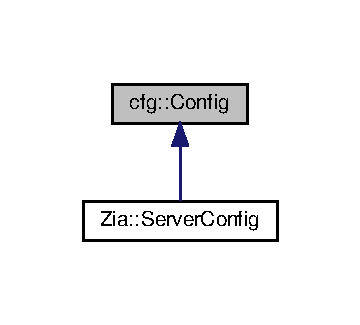
\includegraphics[width=173pt]{classcfg_1_1_config__inherit__graph}
\end{center}
\end{figure}
\subsection*{Public Member Functions}
\begin{DoxyCompactItemize}
\item 
\hyperlink{classcfg_1_1_config_aac0ac15a2f06b8810164441fe08fe490}{Config} (const \hyperlink{namespacecfg_af0aed6e47bd26e91ad7d69467f96caaf}{File\+Descriptor} \&file, const std\+::string \&name)
\begin{DoxyCompactList}\small\item\em Construct a new \hyperlink{classcfg_1_1_config}{Config} object. \end{DoxyCompactList}\item 
virtual \hyperlink{classcfg_1_1_config_a1b74ecb20fb34c56ac3257066e4c065f}{$\sim$\+Config} ()=default
\begin{DoxyCompactList}\small\item\em Destroy the \hyperlink{classcfg_1_1_config}{Config} object. \end{DoxyCompactList}\item 
void \hyperlink{classcfg_1_1_config_a8c2a84783775b02046041628d74be6e7}{load\+Config} (const std\+::filesystem\+::path \&path)
\begin{DoxyCompactList}\small\item\em Load configuration from a given file. \end{DoxyCompactList}\item 
void \hyperlink{classcfg_1_1_config_a622ad4331306ae232060ef6e74fe8134}{update} (const \hyperlink{namespacecfg_a384f743959a9029f7e1c3d11548795de}{File\+Status} \&status)
\item 
void \hyperlink{classcfg_1_1_config_a04f2e4ad0070a73728c4bce7b7dd0c29}{set\+Name} (const std\+::string \&name)
\begin{DoxyCompactList}\small\item\em Set the configuration\textquotesingle{}s name. \end{DoxyCompactList}\item 
const std\+::string \hyperlink{classcfg_1_1_config_ac1fa619b1d5dbd0c3326ac93a4d437bb}{get\+Name} () const noexcept
\begin{DoxyCompactList}\small\item\em Get the configuration\textquotesingle{}s name. \end{DoxyCompactList}\item 
const \hyperlink{namespacecfg_af0aed6e47bd26e91ad7d69467f96caaf}{File\+Descriptor} \hyperlink{classcfg_1_1_config_a76cb1f6d83b6d06eee652c80d32e9084}{get\+File\+Descriptor} () const noexcept
\begin{DoxyCompactList}\small\item\em Get the configuration\textquotesingle{}s file descriptor. \end{DoxyCompactList}\item 
void \hyperlink{classcfg_1_1_config_a4c237371c0ad09ff75d1db7d31a1f362}{set\+Path} (const std\+::filesystem\+::path \&path)
\begin{DoxyCompactList}\small\item\em Set the configuration\textquotesingle{}s file path. \end{DoxyCompactList}\item 
std\+::filesystem\+::path \hyperlink{classcfg_1_1_config_aec545d9dc88130f76bfb6f2a1863b22f}{get\+Path} () const noexcept
\begin{DoxyCompactList}\small\item\em Get the configuration\textquotesingle{}s file path. \end{DoxyCompactList}\item 
void \hyperlink{classcfg_1_1_config_aae2d7dbb7d3d329f1afffef4b95de204}{set\+Timestamp} (const \hyperlink{namespacecfg_aa17d58439174a5af7fb3f37a3cdd6d0b}{Timestamp} \&timestamp)
\begin{DoxyCompactList}\small\item\em Set the configuration\textquotesingle{}s timestamp. \end{DoxyCompactList}\item 
\hyperlink{namespacecfg_aa17d58439174a5af7fb3f37a3cdd6d0b}{Timestamp} \hyperlink{classcfg_1_1_config_acbd974221e2b58f235b596ec3a52c44c}{get\+Timestamp} () const noexcept
\begin{DoxyCompactList}\small\item\em Get the configuration\textquotesingle{}s timestamp. \end{DoxyCompactList}\end{DoxyCompactItemize}


\subsection{Detailed Description}
\hyperlink{classcfg_1_1_config}{Config} abstracts a configuration from a json file. 

Definition at line 83 of file Config.\+hpp.



\subsection{Constructor \& Destructor Documentation}
\mbox{\Hypertarget{classcfg_1_1_config_aac0ac15a2f06b8810164441fe08fe490}\label{classcfg_1_1_config_aac0ac15a2f06b8810164441fe08fe490}} 
\index{cfg\+::\+Config@{cfg\+::\+Config}!Config@{Config}}
\index{Config@{Config}!cfg\+::\+Config@{cfg\+::\+Config}}
\subsubsection{\texorpdfstring{Config()}{Config()}}
{\footnotesize\ttfamily Config\+::\+Config (\begin{DoxyParamCaption}\item[{const \hyperlink{namespacecfg_af0aed6e47bd26e91ad7d69467f96caaf}{File\+Descriptor} \&}]{file,  }\item[{const std\+::string \&}]{name }\end{DoxyParamCaption})}



Construct a new \hyperlink{classcfg_1_1_config}{Config} object. 


\begin{DoxyParams}{Parameters}
{\em file} & File descriptor of the associated json configuration file. \\
\hline
{\em name} & Registration name of the \hyperlink{classcfg_1_1_config}{Config} object. \\
\hline
\end{DoxyParams}


Definition at line 12 of file Config.\+cpp.

\mbox{\Hypertarget{classcfg_1_1_config_a1b74ecb20fb34c56ac3257066e4c065f}\label{classcfg_1_1_config_a1b74ecb20fb34c56ac3257066e4c065f}} 
\index{cfg\+::\+Config@{cfg\+::\+Config}!````~Config@{$\sim$\+Config}}
\index{````~Config@{$\sim$\+Config}!cfg\+::\+Config@{cfg\+::\+Config}}
\subsubsection{\texorpdfstring{$\sim$\+Config()}{~Config()}}
{\footnotesize\ttfamily virtual cfg\+::\+Config\+::$\sim$\+Config (\begin{DoxyParamCaption}{ }\end{DoxyParamCaption})\hspace{0.3cm}{\ttfamily [virtual]}, {\ttfamily [default]}}



Destroy the \hyperlink{classcfg_1_1_config}{Config} object. 



\subsection{Member Function Documentation}
\mbox{\Hypertarget{classcfg_1_1_config_a76cb1f6d83b6d06eee652c80d32e9084}\label{classcfg_1_1_config_a76cb1f6d83b6d06eee652c80d32e9084}} 
\index{cfg\+::\+Config@{cfg\+::\+Config}!get\+File\+Descriptor@{get\+File\+Descriptor}}
\index{get\+File\+Descriptor@{get\+File\+Descriptor}!cfg\+::\+Config@{cfg\+::\+Config}}
\subsubsection{\texorpdfstring{get\+File\+Descriptor()}{getFileDescriptor()}}
{\footnotesize\ttfamily const \hyperlink{namespacecfg_af0aed6e47bd26e91ad7d69467f96caaf}{File\+Descriptor} Config\+::get\+File\+Descriptor (\begin{DoxyParamCaption}{ }\end{DoxyParamCaption}) const\hspace{0.3cm}{\ttfamily [noexcept]}}



Get the configuration\textquotesingle{}s file descriptor. 



Definition at line 60 of file Config.\+cpp.

\mbox{\Hypertarget{classcfg_1_1_config_ac1fa619b1d5dbd0c3326ac93a4d437bb}\label{classcfg_1_1_config_ac1fa619b1d5dbd0c3326ac93a4d437bb}} 
\index{cfg\+::\+Config@{cfg\+::\+Config}!get\+Name@{get\+Name}}
\index{get\+Name@{get\+Name}!cfg\+::\+Config@{cfg\+::\+Config}}
\subsubsection{\texorpdfstring{get\+Name()}{getName()}}
{\footnotesize\ttfamily const std\+::string Config\+::get\+Name (\begin{DoxyParamCaption}{ }\end{DoxyParamCaption}) const\hspace{0.3cm}{\ttfamily [noexcept]}}



Get the configuration\textquotesingle{}s name. 



Definition at line 55 of file Config.\+cpp.

\mbox{\Hypertarget{classcfg_1_1_config_aec545d9dc88130f76bfb6f2a1863b22f}\label{classcfg_1_1_config_aec545d9dc88130f76bfb6f2a1863b22f}} 
\index{cfg\+::\+Config@{cfg\+::\+Config}!get\+Path@{get\+Path}}
\index{get\+Path@{get\+Path}!cfg\+::\+Config@{cfg\+::\+Config}}
\subsubsection{\texorpdfstring{get\+Path()}{getPath()}}
{\footnotesize\ttfamily std\+::filesystem\+::path Config\+::get\+Path (\begin{DoxyParamCaption}{ }\end{DoxyParamCaption}) const\hspace{0.3cm}{\ttfamily [noexcept]}}



Get the configuration\textquotesingle{}s file path. 



Definition at line 70 of file Config.\+cpp.

\mbox{\Hypertarget{classcfg_1_1_config_acbd974221e2b58f235b596ec3a52c44c}\label{classcfg_1_1_config_acbd974221e2b58f235b596ec3a52c44c}} 
\index{cfg\+::\+Config@{cfg\+::\+Config}!get\+Timestamp@{get\+Timestamp}}
\index{get\+Timestamp@{get\+Timestamp}!cfg\+::\+Config@{cfg\+::\+Config}}
\subsubsection{\texorpdfstring{get\+Timestamp()}{getTimestamp()}}
{\footnotesize\ttfamily \hyperlink{namespacecfg_aa17d58439174a5af7fb3f37a3cdd6d0b}{Timestamp} Config\+::get\+Timestamp (\begin{DoxyParamCaption}{ }\end{DoxyParamCaption}) const\hspace{0.3cm}{\ttfamily [noexcept]}}



Get the configuration\textquotesingle{}s timestamp. 



Definition at line 80 of file Config.\+cpp.

\mbox{\Hypertarget{classcfg_1_1_config_a8c2a84783775b02046041628d74be6e7}\label{classcfg_1_1_config_a8c2a84783775b02046041628d74be6e7}} 
\index{cfg\+::\+Config@{cfg\+::\+Config}!load\+Config@{load\+Config}}
\index{load\+Config@{load\+Config}!cfg\+::\+Config@{cfg\+::\+Config}}
\subsubsection{\texorpdfstring{load\+Config()}{loadConfig()}}
{\footnotesize\ttfamily void Config\+::load\+Config (\begin{DoxyParamCaption}\item[{const std\+::filesystem\+::path \&}]{path }\end{DoxyParamCaption})}



Load configuration from a given file. 


\begin{DoxyParams}{Parameters}
{\em path} & Path to the configuration file. \\
\hline
\end{DoxyParams}


Definition at line 20 of file Config.\+cpp.

\mbox{\Hypertarget{classcfg_1_1_config_a04f2e4ad0070a73728c4bce7b7dd0c29}\label{classcfg_1_1_config_a04f2e4ad0070a73728c4bce7b7dd0c29}} 
\index{cfg\+::\+Config@{cfg\+::\+Config}!set\+Name@{set\+Name}}
\index{set\+Name@{set\+Name}!cfg\+::\+Config@{cfg\+::\+Config}}
\subsubsection{\texorpdfstring{set\+Name()}{setName()}}
{\footnotesize\ttfamily void Config\+::set\+Name (\begin{DoxyParamCaption}\item[{const std\+::string \&}]{name }\end{DoxyParamCaption})}



Set the configuration\textquotesingle{}s name. 


\begin{DoxyParams}{Parameters}
{\em name} & Name to set. \\
\hline
\end{DoxyParams}


Definition at line 50 of file Config.\+cpp.

\mbox{\Hypertarget{classcfg_1_1_config_a4c237371c0ad09ff75d1db7d31a1f362}\label{classcfg_1_1_config_a4c237371c0ad09ff75d1db7d31a1f362}} 
\index{cfg\+::\+Config@{cfg\+::\+Config}!set\+Path@{set\+Path}}
\index{set\+Path@{set\+Path}!cfg\+::\+Config@{cfg\+::\+Config}}
\subsubsection{\texorpdfstring{set\+Path()}{setPath()}}
{\footnotesize\ttfamily void Config\+::set\+Path (\begin{DoxyParamCaption}\item[{const std\+::filesystem\+::path \&}]{path }\end{DoxyParamCaption})}



Set the configuration\textquotesingle{}s file path. 


\begin{DoxyParams}{Parameters}
{\em path} & Path to set. \\
\hline
\end{DoxyParams}


Definition at line 65 of file Config.\+cpp.

\mbox{\Hypertarget{classcfg_1_1_config_aae2d7dbb7d3d329f1afffef4b95de204}\label{classcfg_1_1_config_aae2d7dbb7d3d329f1afffef4b95de204}} 
\index{cfg\+::\+Config@{cfg\+::\+Config}!set\+Timestamp@{set\+Timestamp}}
\index{set\+Timestamp@{set\+Timestamp}!cfg\+::\+Config@{cfg\+::\+Config}}
\subsubsection{\texorpdfstring{set\+Timestamp()}{setTimestamp()}}
{\footnotesize\ttfamily void Config\+::set\+Timestamp (\begin{DoxyParamCaption}\item[{const \hyperlink{namespacecfg_aa17d58439174a5af7fb3f37a3cdd6d0b}{Timestamp} \&}]{timestamp }\end{DoxyParamCaption})}



Set the configuration\textquotesingle{}s timestamp. 


\begin{DoxyParams}{Parameters}
{\em timestamp} & Timestamp to set. \\
\hline
\end{DoxyParams}


Definition at line 75 of file Config.\+cpp.

\mbox{\Hypertarget{classcfg_1_1_config_a622ad4331306ae232060ef6e74fe8134}\label{classcfg_1_1_config_a622ad4331306ae232060ef6e74fe8134}} 
\index{cfg\+::\+Config@{cfg\+::\+Config}!update@{update}}
\index{update@{update}!cfg\+::\+Config@{cfg\+::\+Config}}
\subsubsection{\texorpdfstring{update()}{update()}}
{\footnotesize\ttfamily void Config\+::update (\begin{DoxyParamCaption}\item[{const \hyperlink{namespacecfg_a384f743959a9029f7e1c3d11548795de}{File\+Status} \&}]{status }\end{DoxyParamCaption})}



Definition at line 35 of file Config.\+cpp.



The documentation for this class was generated from the following files\+:\begin{DoxyCompactItemize}
\item 
src/config/\hyperlink{_config_8hpp}{Config.\+hpp}\item 
src/config/\hyperlink{_config_8cpp}{Config.\+cpp}\end{DoxyCompactItemize}

\hypertarget{classcfg_1_1_config_manager}{}\section{cfg\+:\+:Config\+Manager Class Reference}
\label{classcfg_1_1_config_manager}\index{cfg\+::\+Config\+Manager@{cfg\+::\+Config\+Manager}}


\hyperlink{classcfg_1_1_config_manager}{Config\+Manager} class to manage the configuration files.  




{\ttfamily \#include $<$Config\+Manager.\+hpp$>$}

\subsection*{Public Types}
\begin{DoxyCompactItemize}
\item 
using \hyperlink{classcfg_1_1_config_manager_a6614f22d32db38ce6d6ed5b351d4f628}{Callback\+Handler} = std\+::function$<$ void()$>$
\begin{DoxyCompactList}\small\item\em Callback handler that stores something\textquotesingle{}s callback function. \end{DoxyCompactList}\item 
using \hyperlink{classcfg_1_1_config_manager_abb7d9a63860843839fa4d8f339f0122b}{Thread\+Ptr} = std\+::shared\+\_\+ptr$<$ std\+::thread $>$
\begin{DoxyCompactList}\small\item\em Thread pointer type, using shared\+\_\+ptr as backend. \end{DoxyCompactList}\item 
using \hyperlink{classcfg_1_1_config_manager_a94ed7fb2c98c2584e0f98326bf65c98f}{Config\+List} = std\+::vector$<$ \hyperlink{namespacecfg_af5f3a3fc2010c76e90bc66696485989f}{Config\+Ptr} $>$
\begin{DoxyCompactList}\small\item\em Vector containing I\+Config modules. \end{DoxyCompactList}\item 
using \hyperlink{classcfg_1_1_config_manager_ac50f6c213e2646aa1c261c431b6fe351}{Config\+Map} = std\+::unordered\+\_\+map$<$ std\+::string, \hyperlink{namespacecfg_aa17d58439174a5af7fb3f37a3cdd6d0b}{Timestamp} $>$
\begin{DoxyCompactList}\small\item\em Unordered\+\_\+map containing I\+Config modules as key and config file timestamp. \end{DoxyCompactList}\end{DoxyCompactItemize}
\subsection*{Public Member Functions}
\begin{DoxyCompactItemize}
\item 
\hyperlink{classcfg_1_1_config_manager_a5434bffe1b9b3a20026e2526601911f2}{Config\+Manager} (const std\+::string \&path)
\begin{DoxyCompactList}\small\item\em Construct a new \hyperlink{classcfg_1_1_config_manager}{Config\+Manager} object. \end{DoxyCompactList}\item 
\hyperlink{classcfg_1_1_config_manager_a7d3d7c10423d969f7544509f6fcca32f}{Config\+Manager} ()
\begin{DoxyCompactList}\small\item\em Construct a new \hyperlink{classcfg_1_1_config_manager}{Config\+Manager} object. \end{DoxyCompactList}\item 
virtual \hyperlink{classcfg_1_1_config_manager_a0b0ce1e9ef223cd18360eaaeecc7e1ab}{$\sim$\+Config\+Manager} ()=default
\begin{DoxyCompactList}\small\item\em Destroy the \hyperlink{classcfg_1_1_config_manager}{Config\+Manager} object. \end{DoxyCompactList}\item 
void \hyperlink{classcfg_1_1_config_manager_addf0e3547d8e4d7dd023c17e43e8176d}{manage} ()
\begin{DoxyCompactList}\small\item\em Set watching variable to true and run watch method in a detached thread. \end{DoxyCompactList}\item 
void \hyperlink{classcfg_1_1_config_manager_ae72f47047d91fa0418391aa99b2383ef}{stop} ()
\begin{DoxyCompactList}\small\item\em Stop watch method and join the detached thread. \end{DoxyCompactList}\item 
void \hyperlink{classcfg_1_1_config_manager_a31f95938b66f996b8e731dada6b4a880}{watch} ()
\begin{DoxyCompactList}\small\item\em Check every X milliseconds for a modification in the configuration path. \end{DoxyCompactList}\item 
void \hyperlink{classcfg_1_1_config_manager_a5c6d63489274c7ddeb88891caea5ca48}{watching} (const bool \&watching)
\begin{DoxyCompactList}\small\item\em Set watching attribute. \end{DoxyCompactList}\item 
const bool \hyperlink{classcfg_1_1_config_manager_a704e8f6b81715a24199f3579a946cad4}{is\+Watching} () const noexcept
\begin{DoxyCompactList}\small\item\em Get watching attribute. \end{DoxyCompactList}\item 
void \hyperlink{classcfg_1_1_config_manager_ad6c55b0413f949cc5002467cbcee3186}{load\+Config\+Dir} (const std\+::string \&path)
\begin{DoxyCompactList}\small\item\em Load all configuration file from a given path. \end{DoxyCompactList}\item 
void \hyperlink{classcfg_1_1_config_manager_a324ba63493aefb579500f7338bd477db}{on\+Config\+Change} (\hyperlink{classcfg_1_1_config_manager_a6614f22d32db38ce6d6ed5b351d4f628}{Callback\+Handler} \&\&handler)
\begin{DoxyCompactList}\small\item\em Callback called when a file has been modified. \end{DoxyCompactList}\item 
void \hyperlink{classcfg_1_1_config_manager_abee2ba9f508be9604bf91d7f90691bcf}{on\+Config\+Erased} (\hyperlink{classcfg_1_1_config_manager_a6614f22d32db38ce6d6ed5b351d4f628}{Callback\+Handler} \&\&handler)
\begin{DoxyCompactList}\small\item\em Callback called when a file has been erased. \end{DoxyCompactList}\item 
void \hyperlink{classcfg_1_1_config_manager_adf39406f57dfd1871ee974dd86d16abc}{set\+Config\+Path} (const std\+::string \&path)
\begin{DoxyCompactList}\small\item\em Set the configuration path. \end{DoxyCompactList}\item 
const std\+::string \hyperlink{classcfg_1_1_config_manager_af80e94a2a93aa7bb16c2fca5249936ac}{get\+Config\+Path} () const noexcept
\begin{DoxyCompactList}\small\item\em Get the configuration path. \end{DoxyCompactList}\item 
void \hyperlink{classcfg_1_1_config_manager_a8a84b0efbaf6446b4c9254386606cda5}{set\+Time\+To\+Sleep} (const \hyperlink{namespacecfg_ab1a8f7060b6dfea6111c4449e81c6f8c}{Time\+Sleep} \&time\+Sleep)
\begin{DoxyCompactList}\small\item\em Set the time to sleep between each watch loop. \end{DoxyCompactList}\item 
const \hyperlink{namespacecfg_ab1a8f7060b6dfea6111c4449e81c6f8c}{Time\+Sleep} \hyperlink{classcfg_1_1_config_manager_a992557430937cec5387d84d44c721f7c}{get\+Time\+To\+Sleep} () const noexcept
\begin{DoxyCompactList}\small\item\em Get the time to sleep between each watch loop. \end{DoxyCompactList}\item 
\hyperlink{namespacecfg_af5f3a3fc2010c76e90bc66696485989f}{Config\+Ptr} \hyperlink{classcfg_1_1_config_manager_aa71c6277d421969606433b77d425d19d}{get\+Config} (const std\+::string \&config\+Name) const
\begin{DoxyCompactList}\small\item\em Get \hyperlink{classcfg_1_1_config}{Config} object from the loaded configs. \end{DoxyCompactList}\end{DoxyCompactItemize}


\subsection{Detailed Description}
\hyperlink{classcfg_1_1_config_manager}{Config\+Manager} class to manage the configuration files. 

Definition at line 28 of file Config\+Manager.\+hpp.



\subsection{Member Typedef Documentation}
\mbox{\Hypertarget{classcfg_1_1_config_manager_a6614f22d32db38ce6d6ed5b351d4f628}\label{classcfg_1_1_config_manager_a6614f22d32db38ce6d6ed5b351d4f628}} 
\index{cfg\+::\+Config\+Manager@{cfg\+::\+Config\+Manager}!Callback\+Handler@{Callback\+Handler}}
\index{Callback\+Handler@{Callback\+Handler}!cfg\+::\+Config\+Manager@{cfg\+::\+Config\+Manager}}
\subsubsection{\texorpdfstring{Callback\+Handler}{CallbackHandler}}
{\footnotesize\ttfamily using \hyperlink{classcfg_1_1_config_manager_a6614f22d32db38ce6d6ed5b351d4f628}{cfg\+::\+Config\+Manager\+::\+Callback\+Handler} =  std\+::function$<$void()$>$}



Callback handler that stores something\textquotesingle{}s callback function. 



Definition at line 34 of file Config\+Manager.\+hpp.

\mbox{\Hypertarget{classcfg_1_1_config_manager_a94ed7fb2c98c2584e0f98326bf65c98f}\label{classcfg_1_1_config_manager_a94ed7fb2c98c2584e0f98326bf65c98f}} 
\index{cfg\+::\+Config\+Manager@{cfg\+::\+Config\+Manager}!Config\+List@{Config\+List}}
\index{Config\+List@{Config\+List}!cfg\+::\+Config\+Manager@{cfg\+::\+Config\+Manager}}
\subsubsection{\texorpdfstring{Config\+List}{ConfigList}}
{\footnotesize\ttfamily using \hyperlink{classcfg_1_1_config_manager_a94ed7fb2c98c2584e0f98326bf65c98f}{cfg\+::\+Config\+Manager\+::\+Config\+List} =  std\+::vector$<$\hyperlink{namespacecfg_af5f3a3fc2010c76e90bc66696485989f}{Config\+Ptr}$>$}



Vector containing I\+Config modules. 



Definition at line 44 of file Config\+Manager.\+hpp.

\mbox{\Hypertarget{classcfg_1_1_config_manager_ac50f6c213e2646aa1c261c431b6fe351}\label{classcfg_1_1_config_manager_ac50f6c213e2646aa1c261c431b6fe351}} 
\index{cfg\+::\+Config\+Manager@{cfg\+::\+Config\+Manager}!Config\+Map@{Config\+Map}}
\index{Config\+Map@{Config\+Map}!cfg\+::\+Config\+Manager@{cfg\+::\+Config\+Manager}}
\subsubsection{\texorpdfstring{Config\+Map}{ConfigMap}}
{\footnotesize\ttfamily using \hyperlink{classcfg_1_1_config_manager_ac50f6c213e2646aa1c261c431b6fe351}{cfg\+::\+Config\+Manager\+::\+Config\+Map} =  std\+::unordered\+\_\+map$<$std\+::string, \hyperlink{namespacecfg_aa17d58439174a5af7fb3f37a3cdd6d0b}{Timestamp}$>$}



Unordered\+\_\+map containing I\+Config modules as key and config file timestamp. 



Definition at line 49 of file Config\+Manager.\+hpp.

\mbox{\Hypertarget{classcfg_1_1_config_manager_abb7d9a63860843839fa4d8f339f0122b}\label{classcfg_1_1_config_manager_abb7d9a63860843839fa4d8f339f0122b}} 
\index{cfg\+::\+Config\+Manager@{cfg\+::\+Config\+Manager}!Thread\+Ptr@{Thread\+Ptr}}
\index{Thread\+Ptr@{Thread\+Ptr}!cfg\+::\+Config\+Manager@{cfg\+::\+Config\+Manager}}
\subsubsection{\texorpdfstring{Thread\+Ptr}{ThreadPtr}}
{\footnotesize\ttfamily using \hyperlink{classcfg_1_1_config_manager_abb7d9a63860843839fa4d8f339f0122b}{cfg\+::\+Config\+Manager\+::\+Thread\+Ptr} =  std\+::shared\+\_\+ptr$<$std\+::thread$>$}



Thread pointer type, using shared\+\_\+ptr as backend. 



Definition at line 39 of file Config\+Manager.\+hpp.



\subsection{Constructor \& Destructor Documentation}
\mbox{\Hypertarget{classcfg_1_1_config_manager_a5434bffe1b9b3a20026e2526601911f2}\label{classcfg_1_1_config_manager_a5434bffe1b9b3a20026e2526601911f2}} 
\index{cfg\+::\+Config\+Manager@{cfg\+::\+Config\+Manager}!Config\+Manager@{Config\+Manager}}
\index{Config\+Manager@{Config\+Manager}!cfg\+::\+Config\+Manager@{cfg\+::\+Config\+Manager}}
\subsubsection{\texorpdfstring{Config\+Manager()}{ConfigManager()}\hspace{0.1cm}{\footnotesize\ttfamily [1/2]}}
{\footnotesize\ttfamily Config\+Manager\+::\+Config\+Manager (\begin{DoxyParamCaption}\item[{const std\+::string \&}]{path }\end{DoxyParamCaption})}



Construct a new \hyperlink{classcfg_1_1_config_manager}{Config\+Manager} object. 


\begin{DoxyParams}{Parameters}
{\em path} & Path to the directory containing configurations files to watch. \\
\hline
\end{DoxyParams}


Definition at line 12 of file Config\+Manager.\+cpp.

\mbox{\Hypertarget{classcfg_1_1_config_manager_a7d3d7c10423d969f7544509f6fcca32f}\label{classcfg_1_1_config_manager_a7d3d7c10423d969f7544509f6fcca32f}} 
\index{cfg\+::\+Config\+Manager@{cfg\+::\+Config\+Manager}!Config\+Manager@{Config\+Manager}}
\index{Config\+Manager@{Config\+Manager}!cfg\+::\+Config\+Manager@{cfg\+::\+Config\+Manager}}
\subsubsection{\texorpdfstring{Config\+Manager()}{ConfigManager()}\hspace{0.1cm}{\footnotesize\ttfamily [2/2]}}
{\footnotesize\ttfamily Config\+Manager\+::\+Config\+Manager (\begin{DoxyParamCaption}{ }\end{DoxyParamCaption})}



Construct a new \hyperlink{classcfg_1_1_config_manager}{Config\+Manager} object. 



Definition at line 23 of file Config\+Manager.\+cpp.

\mbox{\Hypertarget{classcfg_1_1_config_manager_a0b0ce1e9ef223cd18360eaaeecc7e1ab}\label{classcfg_1_1_config_manager_a0b0ce1e9ef223cd18360eaaeecc7e1ab}} 
\index{cfg\+::\+Config\+Manager@{cfg\+::\+Config\+Manager}!````~Config\+Manager@{$\sim$\+Config\+Manager}}
\index{````~Config\+Manager@{$\sim$\+Config\+Manager}!cfg\+::\+Config\+Manager@{cfg\+::\+Config\+Manager}}
\subsubsection{\texorpdfstring{$\sim$\+Config\+Manager()}{~ConfigManager()}}
{\footnotesize\ttfamily virtual cfg\+::\+Config\+Manager\+::$\sim$\+Config\+Manager (\begin{DoxyParamCaption}{ }\end{DoxyParamCaption})\hspace{0.3cm}{\ttfamily [virtual]}, {\ttfamily [default]}}



Destroy the \hyperlink{classcfg_1_1_config_manager}{Config\+Manager} object. 



\subsection{Member Function Documentation}
\mbox{\Hypertarget{classcfg_1_1_config_manager_aa71c6277d421969606433b77d425d19d}\label{classcfg_1_1_config_manager_aa71c6277d421969606433b77d425d19d}} 
\index{cfg\+::\+Config\+Manager@{cfg\+::\+Config\+Manager}!get\+Config@{get\+Config}}
\index{get\+Config@{get\+Config}!cfg\+::\+Config\+Manager@{cfg\+::\+Config\+Manager}}
\subsubsection{\texorpdfstring{get\+Config()}{getConfig()}}
{\footnotesize\ttfamily \hyperlink{namespacecfg_af5f3a3fc2010c76e90bc66696485989f}{Config\+Ptr} Config\+Manager\+::get\+Config (\begin{DoxyParamCaption}\item[{const std\+::string \&}]{config\+Name }\end{DoxyParamCaption}) const}



Get \hyperlink{classcfg_1_1_config}{Config} object from the loaded configs. 


\begin{DoxyParams}{Parameters}
{\em config\+Name} & Name of the \hyperlink{classcfg_1_1_config}{Config} object wanted.\\
\hline
\end{DoxyParams}
\begin{DoxyReturn}{Returns}
Wanted Config\+Ptr. 
\end{DoxyReturn}


Definition at line 126 of file Config\+Manager.\+cpp.

\mbox{\Hypertarget{classcfg_1_1_config_manager_af80e94a2a93aa7bb16c2fca5249936ac}\label{classcfg_1_1_config_manager_af80e94a2a93aa7bb16c2fca5249936ac}} 
\index{cfg\+::\+Config\+Manager@{cfg\+::\+Config\+Manager}!get\+Config\+Path@{get\+Config\+Path}}
\index{get\+Config\+Path@{get\+Config\+Path}!cfg\+::\+Config\+Manager@{cfg\+::\+Config\+Manager}}
\subsubsection{\texorpdfstring{get\+Config\+Path()}{getConfigPath()}}
{\footnotesize\ttfamily const std\+::string Config\+Manager\+::get\+Config\+Path (\begin{DoxyParamCaption}{ }\end{DoxyParamCaption}) const\hspace{0.3cm}{\ttfamily [noexcept]}}



Get the configuration path. 

\begin{DoxyReturn}{Returns}
The configuration path as a std\+::string. 
\end{DoxyReturn}


Definition at line 101 of file Config\+Manager.\+cpp.

\mbox{\Hypertarget{classcfg_1_1_config_manager_a992557430937cec5387d84d44c721f7c}\label{classcfg_1_1_config_manager_a992557430937cec5387d84d44c721f7c}} 
\index{cfg\+::\+Config\+Manager@{cfg\+::\+Config\+Manager}!get\+Time\+To\+Sleep@{get\+Time\+To\+Sleep}}
\index{get\+Time\+To\+Sleep@{get\+Time\+To\+Sleep}!cfg\+::\+Config\+Manager@{cfg\+::\+Config\+Manager}}
\subsubsection{\texorpdfstring{get\+Time\+To\+Sleep()}{getTimeToSleep()}}
{\footnotesize\ttfamily const \hyperlink{namespacecfg_ab1a8f7060b6dfea6111c4449e81c6f8c}{Time\+Sleep} Config\+Manager\+::get\+Time\+To\+Sleep (\begin{DoxyParamCaption}{ }\end{DoxyParamCaption}) const\hspace{0.3cm}{\ttfamily [noexcept]}}



Get the time to sleep between each watch loop. 

\begin{DoxyReturn}{Returns}
The time to sleep as a Time\+Sleep. 
\end{DoxyReturn}


Definition at line 111 of file Config\+Manager.\+cpp.

\mbox{\Hypertarget{classcfg_1_1_config_manager_a704e8f6b81715a24199f3579a946cad4}\label{classcfg_1_1_config_manager_a704e8f6b81715a24199f3579a946cad4}} 
\index{cfg\+::\+Config\+Manager@{cfg\+::\+Config\+Manager}!is\+Watching@{is\+Watching}}
\index{is\+Watching@{is\+Watching}!cfg\+::\+Config\+Manager@{cfg\+::\+Config\+Manager}}
\subsubsection{\texorpdfstring{is\+Watching()}{isWatching()}}
{\footnotesize\ttfamily const bool Config\+Manager\+::is\+Watching (\begin{DoxyParamCaption}{ }\end{DoxyParamCaption}) const\hspace{0.3cm}{\ttfamily [noexcept]}}



Get watching attribute. 

\begin{DoxyReturn}{Returns}
Watching attribute as a boolean. 
\end{DoxyReturn}


Definition at line 81 of file Config\+Manager.\+cpp.

\mbox{\Hypertarget{classcfg_1_1_config_manager_ad6c55b0413f949cc5002467cbcee3186}\label{classcfg_1_1_config_manager_ad6c55b0413f949cc5002467cbcee3186}} 
\index{cfg\+::\+Config\+Manager@{cfg\+::\+Config\+Manager}!load\+Config\+Dir@{load\+Config\+Dir}}
\index{load\+Config\+Dir@{load\+Config\+Dir}!cfg\+::\+Config\+Manager@{cfg\+::\+Config\+Manager}}
\subsubsection{\texorpdfstring{load\+Config\+Dir()}{loadConfigDir()}}
{\footnotesize\ttfamily void Config\+Manager\+::load\+Config\+Dir (\begin{DoxyParamCaption}\item[{const std\+::string \&}]{path }\end{DoxyParamCaption})}



Load all configuration file from a given path. 


\begin{DoxyParams}{Parameters}
{\em path} & Path where to load the configuration files. \\
\hline
\end{DoxyParams}


Definition at line 86 of file Config\+Manager.\+cpp.

\mbox{\Hypertarget{classcfg_1_1_config_manager_addf0e3547d8e4d7dd023c17e43e8176d}\label{classcfg_1_1_config_manager_addf0e3547d8e4d7dd023c17e43e8176d}} 
\index{cfg\+::\+Config\+Manager@{cfg\+::\+Config\+Manager}!manage@{manage}}
\index{manage@{manage}!cfg\+::\+Config\+Manager@{cfg\+::\+Config\+Manager}}
\subsubsection{\texorpdfstring{manage()}{manage()}}
{\footnotesize\ttfamily void Config\+Manager\+::manage (\begin{DoxyParamCaption}{ }\end{DoxyParamCaption})}



Set watching variable to true and run watch method in a detached thread. 



Definition at line 34 of file Config\+Manager.\+cpp.

\mbox{\Hypertarget{classcfg_1_1_config_manager_a324ba63493aefb579500f7338bd477db}\label{classcfg_1_1_config_manager_a324ba63493aefb579500f7338bd477db}} 
\index{cfg\+::\+Config\+Manager@{cfg\+::\+Config\+Manager}!on\+Config\+Change@{on\+Config\+Change}}
\index{on\+Config\+Change@{on\+Config\+Change}!cfg\+::\+Config\+Manager@{cfg\+::\+Config\+Manager}}
\subsubsection{\texorpdfstring{on\+Config\+Change()}{onConfigChange()}}
{\footnotesize\ttfamily void Config\+Manager\+::on\+Config\+Change (\begin{DoxyParamCaption}\item[{\hyperlink{classcfg_1_1_config_manager_a6614f22d32db38ce6d6ed5b351d4f628}{Callback\+Handler} \&\&}]{handler }\end{DoxyParamCaption})}



Callback called when a file has been modified. 


\begin{DoxyParams}{Parameters}
{\em handler} & Callback function. \\
\hline
\end{DoxyParams}


Definition at line 116 of file Config\+Manager.\+cpp.

\mbox{\Hypertarget{classcfg_1_1_config_manager_abee2ba9f508be9604bf91d7f90691bcf}\label{classcfg_1_1_config_manager_abee2ba9f508be9604bf91d7f90691bcf}} 
\index{cfg\+::\+Config\+Manager@{cfg\+::\+Config\+Manager}!on\+Config\+Erased@{on\+Config\+Erased}}
\index{on\+Config\+Erased@{on\+Config\+Erased}!cfg\+::\+Config\+Manager@{cfg\+::\+Config\+Manager}}
\subsubsection{\texorpdfstring{on\+Config\+Erased()}{onConfigErased()}}
{\footnotesize\ttfamily void Config\+Manager\+::on\+Config\+Erased (\begin{DoxyParamCaption}\item[{\hyperlink{classcfg_1_1_config_manager_a6614f22d32db38ce6d6ed5b351d4f628}{Callback\+Handler} \&\&}]{handler }\end{DoxyParamCaption})}



Callback called when a file has been erased. 


\begin{DoxyParams}{Parameters}
{\em handler} & Callback function \\
\hline
\end{DoxyParams}


Definition at line 121 of file Config\+Manager.\+cpp.

\mbox{\Hypertarget{classcfg_1_1_config_manager_adf39406f57dfd1871ee974dd86d16abc}\label{classcfg_1_1_config_manager_adf39406f57dfd1871ee974dd86d16abc}} 
\index{cfg\+::\+Config\+Manager@{cfg\+::\+Config\+Manager}!set\+Config\+Path@{set\+Config\+Path}}
\index{set\+Config\+Path@{set\+Config\+Path}!cfg\+::\+Config\+Manager@{cfg\+::\+Config\+Manager}}
\subsubsection{\texorpdfstring{set\+Config\+Path()}{setConfigPath()}}
{\footnotesize\ttfamily void Config\+Manager\+::set\+Config\+Path (\begin{DoxyParamCaption}\item[{const std\+::string \&}]{path }\end{DoxyParamCaption})}



Set the configuration path. 


\begin{DoxyParams}{Parameters}
{\em path} & Path where the configuration files are. \\
\hline
\end{DoxyParams}


Definition at line 96 of file Config\+Manager.\+cpp.

\mbox{\Hypertarget{classcfg_1_1_config_manager_a8a84b0efbaf6446b4c9254386606cda5}\label{classcfg_1_1_config_manager_a8a84b0efbaf6446b4c9254386606cda5}} 
\index{cfg\+::\+Config\+Manager@{cfg\+::\+Config\+Manager}!set\+Time\+To\+Sleep@{set\+Time\+To\+Sleep}}
\index{set\+Time\+To\+Sleep@{set\+Time\+To\+Sleep}!cfg\+::\+Config\+Manager@{cfg\+::\+Config\+Manager}}
\subsubsection{\texorpdfstring{set\+Time\+To\+Sleep()}{setTimeToSleep()}}
{\footnotesize\ttfamily void Config\+Manager\+::set\+Time\+To\+Sleep (\begin{DoxyParamCaption}\item[{const \hyperlink{namespacecfg_ab1a8f7060b6dfea6111c4449e81c6f8c}{Time\+Sleep} \&}]{time\+Sleep }\end{DoxyParamCaption})}



Set the time to sleep between each watch loop. 


\begin{DoxyParams}{Parameters}
{\em time\+Sleep} & Time to sleep in milliseconds. \\
\hline
\end{DoxyParams}


Definition at line 106 of file Config\+Manager.\+cpp.

\mbox{\Hypertarget{classcfg_1_1_config_manager_ae72f47047d91fa0418391aa99b2383ef}\label{classcfg_1_1_config_manager_ae72f47047d91fa0418391aa99b2383ef}} 
\index{cfg\+::\+Config\+Manager@{cfg\+::\+Config\+Manager}!stop@{stop}}
\index{stop@{stop}!cfg\+::\+Config\+Manager@{cfg\+::\+Config\+Manager}}
\subsubsection{\texorpdfstring{stop()}{stop()}}
{\footnotesize\ttfamily void Config\+Manager\+::stop (\begin{DoxyParamCaption}{ }\end{DoxyParamCaption})}



Stop watch method and join the detached thread. 



Definition at line 41 of file Config\+Manager.\+cpp.

\mbox{\Hypertarget{classcfg_1_1_config_manager_a31f95938b66f996b8e731dada6b4a880}\label{classcfg_1_1_config_manager_a31f95938b66f996b8e731dada6b4a880}} 
\index{cfg\+::\+Config\+Manager@{cfg\+::\+Config\+Manager}!watch@{watch}}
\index{watch@{watch}!cfg\+::\+Config\+Manager@{cfg\+::\+Config\+Manager}}
\subsubsection{\texorpdfstring{watch()}{watch()}}
{\footnotesize\ttfamily void Config\+Manager\+::watch (\begin{DoxyParamCaption}{ }\end{DoxyParamCaption})}



Check every X milliseconds for a modification in the configuration path. 


\begin{DoxyItemize}
\item If a file is modified, matching config will be reloaded.
\item If a file is deleted, matching config will be removed from the Config\+List. 
\end{DoxyItemize}

Definition at line 47 of file Config\+Manager.\+cpp.

\mbox{\Hypertarget{classcfg_1_1_config_manager_a5c6d63489274c7ddeb88891caea5ca48}\label{classcfg_1_1_config_manager_a5c6d63489274c7ddeb88891caea5ca48}} 
\index{cfg\+::\+Config\+Manager@{cfg\+::\+Config\+Manager}!watching@{watching}}
\index{watching@{watching}!cfg\+::\+Config\+Manager@{cfg\+::\+Config\+Manager}}
\subsubsection{\texorpdfstring{watching()}{watching()}}
{\footnotesize\ttfamily void Config\+Manager\+::watching (\begin{DoxyParamCaption}\item[{const bool \&}]{watching }\end{DoxyParamCaption})}



Set watching attribute. 


\begin{DoxyParams}{Parameters}
{\em watching} & Boolean. \\
\hline
\end{DoxyParams}


Definition at line 76 of file Config\+Manager.\+cpp.



The documentation for this class was generated from the following files\+:\begin{DoxyCompactItemize}
\item 
src/config/\hyperlink{_config_manager_8hpp}{Config\+Manager.\+hpp}\item 
src/config/\hyperlink{_config_manager_8cpp}{Config\+Manager.\+cpp}\end{DoxyCompactItemize}

\hypertarget{class_zia_1_1_connection}{}\section{Zia\+:\+:Connection Class Reference}
\label{class_zia_1_1_connection}\index{Zia\+::\+Connection@{Zia\+::\+Connection}}


\hyperlink{class_zia_1_1_connection}{Connection} class to manage the connection.  




{\ttfamily \#include $<$Connection.\+hpp$>$}



Inheritance diagram for Zia\+:\+:Connection\+:\nopagebreak
\begin{figure}[H]
\begin{center}
\leavevmode
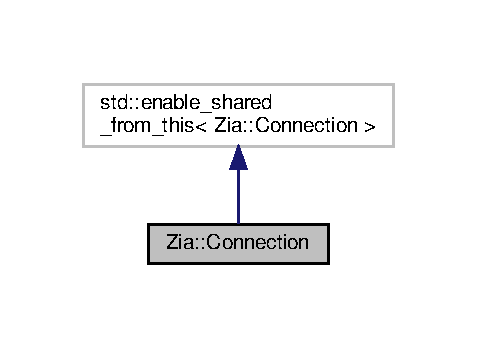
\includegraphics[width=229pt]{class_zia_1_1_connection__inherit__graph}
\end{center}
\end{figure}


Collaboration diagram for Zia\+:\+:Connection\+:\nopagebreak
\begin{figure}[H]
\begin{center}
\leavevmode
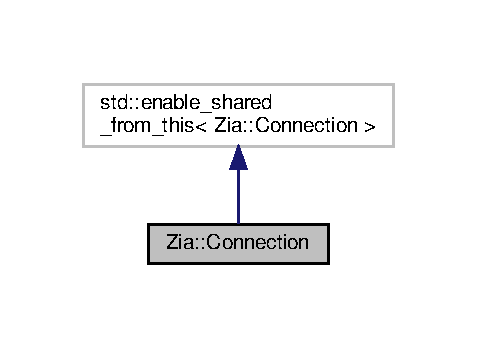
\includegraphics[width=229pt]{class_zia_1_1_connection__coll__graph}
\end{center}
\end{figure}
\subsection*{Public Types}
\begin{DoxyCompactItemize}
\item 
using \hyperlink{class_zia_1_1_connection_a1b74e276e0f3aa8dbabdaed80a0936e6}{socket} = boost\+::asio\+::ip\+::tcp\+::socket
\end{DoxyCompactItemize}
\subsection*{Public Member Functions}
\begin{DoxyCompactItemize}
\item 
\hyperlink{class_zia_1_1_connection_a06a6c69bf205afa9868169a1435129c1}{Connection} (void)=delete
\begin{DoxyCompactList}\small\item\em Contructor of the \hyperlink{class_zia_1_1_connection}{Connection} class. \end{DoxyCompactList}\item 
\hyperlink{class_zia_1_1_connection_a61438cdd01805cd466d1382eafcb1576}{Connection} (\hyperlink{class_zia_1_1_connection_a1b74e276e0f3aa8dbabdaed80a0936e6}{socket} sock, \hyperlink{class_zia_1_1_connection_manager}{Connection\+Manager} \&connection\+Manager, o\+Z\+::\+Pipeline \&pipeline, bool encryption=false)
\begin{DoxyCompactList}\small\item\em Contructor of the \hyperlink{class_zia_1_1_connection}{Connection} class. \end{DoxyCompactList}\item 
void \hyperlink{class_zia_1_1_connection_af7bae27ea5870ef9efc6775d38012aa4}{start} (void)
\begin{DoxyCompactList}\small\item\em Start the connection between browser and serv (client) \end{DoxyCompactList}\item 
void \hyperlink{class_zia_1_1_connection_ac9704053c3b7f919d71255b1ce30cc63}{stop} (void)
\begin{DoxyCompactList}\small\item\em Stop the connection between browser and serv (client) \end{DoxyCompactList}\end{DoxyCompactItemize}


\subsection{Detailed Description}
\hyperlink{class_zia_1_1_connection}{Connection} class to manage the connection. 

Definition at line 25 of file Connection.\+hpp.



\subsection{Member Typedef Documentation}
\mbox{\Hypertarget{class_zia_1_1_connection_a1b74e276e0f3aa8dbabdaed80a0936e6}\label{class_zia_1_1_connection_a1b74e276e0f3aa8dbabdaed80a0936e6}} 
\index{Zia\+::\+Connection@{Zia\+::\+Connection}!socket@{socket}}
\index{socket@{socket}!Zia\+::\+Connection@{Zia\+::\+Connection}}
\subsubsection{\texorpdfstring{socket}{socket}}
{\footnotesize\ttfamily using \hyperlink{class_zia_1_1_connection_a1b74e276e0f3aa8dbabdaed80a0936e6}{Zia\+::\+Connection\+::socket} =  boost\+::asio\+::ip\+::tcp\+::socket}



Definition at line 28 of file Connection.\+hpp.



\subsection{Constructor \& Destructor Documentation}
\mbox{\Hypertarget{class_zia_1_1_connection_a06a6c69bf205afa9868169a1435129c1}\label{class_zia_1_1_connection_a06a6c69bf205afa9868169a1435129c1}} 
\index{Zia\+::\+Connection@{Zia\+::\+Connection}!Connection@{Connection}}
\index{Connection@{Connection}!Zia\+::\+Connection@{Zia\+::\+Connection}}
\subsubsection{\texorpdfstring{Connection()}{Connection()}\hspace{0.1cm}{\footnotesize\ttfamily [1/2]}}
{\footnotesize\ttfamily Zia\+::\+Connection\+::\+Connection (\begin{DoxyParamCaption}\item[{void}]{ }\end{DoxyParamCaption})\hspace{0.3cm}{\ttfamily [delete]}}



Contructor of the \hyperlink{class_zia_1_1_connection}{Connection} class. 

\mbox{\Hypertarget{class_zia_1_1_connection_a61438cdd01805cd466d1382eafcb1576}\label{class_zia_1_1_connection_a61438cdd01805cd466d1382eafcb1576}} 
\index{Zia\+::\+Connection@{Zia\+::\+Connection}!Connection@{Connection}}
\index{Connection@{Connection}!Zia\+::\+Connection@{Zia\+::\+Connection}}
\subsubsection{\texorpdfstring{Connection()}{Connection()}\hspace{0.1cm}{\footnotesize\ttfamily [2/2]}}
{\footnotesize\ttfamily Zia\+::\+Connection\+::\+Connection (\begin{DoxyParamCaption}\item[{\hyperlink{class_zia_1_1_connection_a1b74e276e0f3aa8dbabdaed80a0936e6}{socket}}]{sock,  }\item[{\hyperlink{class_zia_1_1_connection_manager}{Connection\+Manager} \&}]{connection\+Manager,  }\item[{o\+Z\+::\+Pipeline \&}]{pipeline,  }\item[{bool}]{encryption = {\ttfamily false} }\end{DoxyParamCaption})}



Contructor of the \hyperlink{class_zia_1_1_connection}{Connection} class. 


\begin{DoxyParams}{Parameters}
{\em sock} & Socket accepted by the serveur \\
\hline
{\em connection\+Manager} & \hyperlink{class_zia_1_1_connection}{Connection} manager of the server \\
\hline
{\em pipeline} & \hyperlink{class_zia_1_1_server}{Server}\textquotesingle{}s pipeline use for modif the context \\
\hline
{\em encryption} & Bool use to know if this will be in https or not \\
\hline
\end{DoxyParams}


Definition at line 17 of file Connection.\+cpp.



\subsection{Member Function Documentation}
\mbox{\Hypertarget{class_zia_1_1_connection_af7bae27ea5870ef9efc6775d38012aa4}\label{class_zia_1_1_connection_af7bae27ea5870ef9efc6775d38012aa4}} 
\index{Zia\+::\+Connection@{Zia\+::\+Connection}!start@{start}}
\index{start@{start}!Zia\+::\+Connection@{Zia\+::\+Connection}}
\subsubsection{\texorpdfstring{start()}{start()}}
{\footnotesize\ttfamily void Zia\+::\+Connection\+::start (\begin{DoxyParamCaption}\item[{void}]{ }\end{DoxyParamCaption})}



Start the connection between browser and serv (client) 



Definition at line 26 of file Connection.\+cpp.

\mbox{\Hypertarget{class_zia_1_1_connection_ac9704053c3b7f919d71255b1ce30cc63}\label{class_zia_1_1_connection_ac9704053c3b7f919d71255b1ce30cc63}} 
\index{Zia\+::\+Connection@{Zia\+::\+Connection}!stop@{stop}}
\index{stop@{stop}!Zia\+::\+Connection@{Zia\+::\+Connection}}
\subsubsection{\texorpdfstring{stop()}{stop()}}
{\footnotesize\ttfamily void Zia\+::\+Connection\+::stop (\begin{DoxyParamCaption}\item[{void}]{ }\end{DoxyParamCaption})}



Stop the connection between browser and serv (client) 



Definition at line 139 of file Connection.\+cpp.



The documentation for this class was generated from the following files\+:\begin{DoxyCompactItemize}
\item 
src/server/\hyperlink{_connection_8hpp}{Connection.\+hpp}\item 
src/server/\hyperlink{_connection_8cpp}{Connection.\+cpp}\end{DoxyCompactItemize}

\hypertarget{class_zia_1_1_connection_manager}{}\section{Zia\+:\+:Connection\+Manager Class Reference}
\label{class_zia_1_1_connection_manager}\index{Zia\+::\+Connection\+Manager@{Zia\+::\+Connection\+Manager}}


\hyperlink{class_zia_1_1_connection_manager}{Connection\+Manager} class to manage the connection.  




{\ttfamily \#include $<$Connection\+Manager.\+hpp$>$}

\subsection*{Public Member Functions}
\begin{DoxyCompactItemize}
\item 
\hyperlink{class_zia_1_1_connection_manager_a863585668f747d6fb35b15b12f6fb4a4}{Connection\+Manager} ()=default
\begin{DoxyCompactList}\small\item\em Cronstructor for the connection manager. \end{DoxyCompactList}\item 
void \hyperlink{class_zia_1_1_connection_manager_a556bcbe3969171deba4900c08feb7d93}{add\+Client} (\hyperlink{_connection_manager_8hpp_a0e374529952c927bd9f59c9acbccf624}{Connection\+Ptr} client)
\begin{DoxyCompactList}\small\item\em Add a client give to the manager in the list. \end{DoxyCompactList}\item 
void \hyperlink{class_zia_1_1_connection_manager_a61efd54810ec831b994c7ef148bec2ae}{erase\+Client} (\hyperlink{_connection_manager_8hpp_a0e374529952c927bd9f59c9acbccf624}{Connection\+Ptr} client)
\begin{DoxyCompactList}\small\item\em Remove a client give to the manager to the list. \end{DoxyCompactList}\item 
void \hyperlink{class_zia_1_1_connection_manager_ac1db00d9a69520616bc20e0ac1ea311f}{erase\+All} (void)
\begin{DoxyCompactList}\small\item\em Add a client give to the manager in the list. \end{DoxyCompactList}\end{DoxyCompactItemize}


\subsection{Detailed Description}
\hyperlink{class_zia_1_1_connection_manager}{Connection\+Manager} class to manage the connection. 

Definition at line 24 of file Connection\+Manager.\+hpp.



\subsection{Constructor \& Destructor Documentation}
\mbox{\Hypertarget{class_zia_1_1_connection_manager_a863585668f747d6fb35b15b12f6fb4a4}\label{class_zia_1_1_connection_manager_a863585668f747d6fb35b15b12f6fb4a4}} 
\index{Zia\+::\+Connection\+Manager@{Zia\+::\+Connection\+Manager}!Connection\+Manager@{Connection\+Manager}}
\index{Connection\+Manager@{Connection\+Manager}!Zia\+::\+Connection\+Manager@{Zia\+::\+Connection\+Manager}}
\subsubsection{\texorpdfstring{Connection\+Manager()}{ConnectionManager()}}
{\footnotesize\ttfamily Zia\+::\+Connection\+Manager\+::\+Connection\+Manager (\begin{DoxyParamCaption}{ }\end{DoxyParamCaption})\hspace{0.3cm}{\ttfamily [default]}}



Cronstructor for the connection manager. 



\subsection{Member Function Documentation}
\mbox{\Hypertarget{class_zia_1_1_connection_manager_a556bcbe3969171deba4900c08feb7d93}\label{class_zia_1_1_connection_manager_a556bcbe3969171deba4900c08feb7d93}} 
\index{Zia\+::\+Connection\+Manager@{Zia\+::\+Connection\+Manager}!add\+Client@{add\+Client}}
\index{add\+Client@{add\+Client}!Zia\+::\+Connection\+Manager@{Zia\+::\+Connection\+Manager}}
\subsubsection{\texorpdfstring{add\+Client()}{addClient()}}
{\footnotesize\ttfamily void Zia\+::\+Connection\+Manager\+::add\+Client (\begin{DoxyParamCaption}\item[{\hyperlink{_connection_manager_8hpp_a0e374529952c927bd9f59c9acbccf624}{Connection\+Ptr}}]{client }\end{DoxyParamCaption})}



Add a client give to the manager in the list. 


\begin{DoxyParams}{Parameters}
{\em client} & Pointer on the client \\
\hline
\end{DoxyParams}


Definition at line 11 of file Connection\+Manager.\+cpp.

\mbox{\Hypertarget{class_zia_1_1_connection_manager_ac1db00d9a69520616bc20e0ac1ea311f}\label{class_zia_1_1_connection_manager_ac1db00d9a69520616bc20e0ac1ea311f}} 
\index{Zia\+::\+Connection\+Manager@{Zia\+::\+Connection\+Manager}!erase\+All@{erase\+All}}
\index{erase\+All@{erase\+All}!Zia\+::\+Connection\+Manager@{Zia\+::\+Connection\+Manager}}
\subsubsection{\texorpdfstring{erase\+All()}{eraseAll()}}
{\footnotesize\ttfamily void Zia\+::\+Connection\+Manager\+::erase\+All (\begin{DoxyParamCaption}\item[{void}]{ }\end{DoxyParamCaption})}



Add a client give to the manager in the list. 



Definition at line 23 of file Connection\+Manager.\+cpp.

\mbox{\Hypertarget{class_zia_1_1_connection_manager_a61efd54810ec831b994c7ef148bec2ae}\label{class_zia_1_1_connection_manager_a61efd54810ec831b994c7ef148bec2ae}} 
\index{Zia\+::\+Connection\+Manager@{Zia\+::\+Connection\+Manager}!erase\+Client@{erase\+Client}}
\index{erase\+Client@{erase\+Client}!Zia\+::\+Connection\+Manager@{Zia\+::\+Connection\+Manager}}
\subsubsection{\texorpdfstring{erase\+Client()}{eraseClient()}}
{\footnotesize\ttfamily void Zia\+::\+Connection\+Manager\+::erase\+Client (\begin{DoxyParamCaption}\item[{\hyperlink{_connection_manager_8hpp_a0e374529952c927bd9f59c9acbccf624}{Connection\+Ptr}}]{client }\end{DoxyParamCaption})}



Remove a client give to the manager to the list. 


\begin{DoxyParams}{Parameters}
{\em client} & Pointer on the client \\
\hline
\end{DoxyParams}


Definition at line 17 of file Connection\+Manager.\+cpp.



The documentation for this class was generated from the following files\+:\begin{DoxyCompactItemize}
\item 
src/server/\hyperlink{_connection_manager_8hpp}{Connection\+Manager.\+hpp}\item 
src/server/\hyperlink{_connection_manager_8cpp}{Connection\+Manager.\+cpp}\end{DoxyCompactItemize}

\hypertarget{classtls_1_1_env_manager}{}\section{tls\+:\+:Env\+Manager Class Reference}
\label{classtls_1_1_env_manager}\index{tls\+::\+Env\+Manager@{tls\+::\+Env\+Manager}}


\hyperlink{classtls_1_1_env_manager}{Env\+Manager} class to manage environment variables.  




{\ttfamily \#include $<$Env\+Manager.\+hpp$>$}

\subsection*{Public Member Functions}
\begin{DoxyCompactItemize}
\item 
\hyperlink{classtls_1_1_env_manager_a73654081360600e2dd650eea02f82a23}{Env\+Manager} ()
\begin{DoxyCompactList}\small\item\em Construct a new \hyperlink{classtls_1_1_env_manager}{Env\+Manager} object. \end{DoxyCompactList}\item 
\hyperlink{classtls_1_1_env_manager_ad603a242e488ddbda5a54b23aefe2013}{Env\+Manager} (const std\+::filesystem\+::path \&config\+\_\+path)
\begin{DoxyCompactList}\small\item\em Construct a new \hyperlink{classtls_1_1_env_manager}{Env\+Manager} object. \end{DoxyCompactList}\item 
\hyperlink{classtls_1_1_env_manager_aaff18dcf5a41cefdaa1a5b2123a456a0}{$\sim$\+Env\+Manager} ()=default
\begin{DoxyCompactList}\small\item\em Destroy the \hyperlink{classtls_1_1_env_manager}{Env\+Manager} object. \end{DoxyCompactList}\item 
void \hyperlink{classtls_1_1_env_manager_ad48562c6efa024230850b73d9d6361fb}{load\+Env} (const std\+::filesystem\+::path \&config\+\_\+path=\char`\"{}\char`\"{})
\begin{DoxyCompactList}\small\item\em Set a list of environment variable from a json file. \end{DoxyCompactList}\end{DoxyCompactItemize}
\subsection*{Static Public Member Functions}
\begin{DoxyCompactItemize}
\item 
static void \hyperlink{classtls_1_1_env_manager_a560e9c9885ae4e656eb7121adc4cbc9a}{set\+Env} (const std\+::string \&name, const std\+::string \&value)
\begin{DoxyCompactList}\small\item\em Set an environment variable. \end{DoxyCompactList}\item 
static const std\+::string \hyperlink{classtls_1_1_env_manager_a505529a47f05f2450594da617d627936}{get\+Env} (const std\+::string \&name)
\begin{DoxyCompactList}\small\item\em Get an environment variable. \end{DoxyCompactList}\end{DoxyCompactItemize}


\subsection{Detailed Description}
\hyperlink{classtls_1_1_env_manager}{Env\+Manager} class to manage environment variables. 

Definition at line 19 of file Env\+Manager.\+hpp.



\subsection{Constructor \& Destructor Documentation}
\mbox{\Hypertarget{classtls_1_1_env_manager_a73654081360600e2dd650eea02f82a23}\label{classtls_1_1_env_manager_a73654081360600e2dd650eea02f82a23}} 
\index{tls\+::\+Env\+Manager@{tls\+::\+Env\+Manager}!Env\+Manager@{Env\+Manager}}
\index{Env\+Manager@{Env\+Manager}!tls\+::\+Env\+Manager@{tls\+::\+Env\+Manager}}
\subsubsection{\texorpdfstring{Env\+Manager()}{EnvManager()}\hspace{0.1cm}{\footnotesize\ttfamily [1/2]}}
{\footnotesize\ttfamily Env\+Manager\+::\+Env\+Manager (\begin{DoxyParamCaption}{ }\end{DoxyParamCaption})}



Construct a new \hyperlink{classtls_1_1_env_manager}{Env\+Manager} object. 



Definition at line 12 of file Env\+Manager.\+cpp.

\mbox{\Hypertarget{classtls_1_1_env_manager_ad603a242e488ddbda5a54b23aefe2013}\label{classtls_1_1_env_manager_ad603a242e488ddbda5a54b23aefe2013}} 
\index{tls\+::\+Env\+Manager@{tls\+::\+Env\+Manager}!Env\+Manager@{Env\+Manager}}
\index{Env\+Manager@{Env\+Manager}!tls\+::\+Env\+Manager@{tls\+::\+Env\+Manager}}
\subsubsection{\texorpdfstring{Env\+Manager()}{EnvManager()}\hspace{0.1cm}{\footnotesize\ttfamily [2/2]}}
{\footnotesize\ttfamily Env\+Manager\+::\+Env\+Manager (\begin{DoxyParamCaption}\item[{const std\+::filesystem\+::path \&}]{config\+\_\+path }\end{DoxyParamCaption})}



Construct a new \hyperlink{classtls_1_1_env_manager}{Env\+Manager} object. 


\begin{DoxyParams}{Parameters}
{\em config\+\_\+path} & Path to a json configuration file. \\
\hline
\end{DoxyParams}


Definition at line 18 of file Env\+Manager.\+cpp.

\mbox{\Hypertarget{classtls_1_1_env_manager_aaff18dcf5a41cefdaa1a5b2123a456a0}\label{classtls_1_1_env_manager_aaff18dcf5a41cefdaa1a5b2123a456a0}} 
\index{tls\+::\+Env\+Manager@{tls\+::\+Env\+Manager}!````~Env\+Manager@{$\sim$\+Env\+Manager}}
\index{````~Env\+Manager@{$\sim$\+Env\+Manager}!tls\+::\+Env\+Manager@{tls\+::\+Env\+Manager}}
\subsubsection{\texorpdfstring{$\sim$\+Env\+Manager()}{~EnvManager()}}
{\footnotesize\ttfamily tls\+::\+Env\+Manager\+::$\sim$\+Env\+Manager (\begin{DoxyParamCaption}{ }\end{DoxyParamCaption})\hspace{0.3cm}{\ttfamily [default]}}



Destroy the \hyperlink{classtls_1_1_env_manager}{Env\+Manager} object. 



\subsection{Member Function Documentation}
\mbox{\Hypertarget{classtls_1_1_env_manager_a505529a47f05f2450594da617d627936}\label{classtls_1_1_env_manager_a505529a47f05f2450594da617d627936}} 
\index{tls\+::\+Env\+Manager@{tls\+::\+Env\+Manager}!get\+Env@{get\+Env}}
\index{get\+Env@{get\+Env}!tls\+::\+Env\+Manager@{tls\+::\+Env\+Manager}}
\subsubsection{\texorpdfstring{get\+Env()}{getEnv()}}
{\footnotesize\ttfamily const std\+::string Env\+Manager\+::get\+Env (\begin{DoxyParamCaption}\item[{const std\+::string \&}]{name }\end{DoxyParamCaption})\hspace{0.3cm}{\ttfamily [static]}}



Get an environment variable. 


\begin{DoxyParams}{Parameters}
{\em name} & Name of the variable to retrieve.\\
\hline
\end{DoxyParams}
\begin{DoxyReturn}{Returns}
Value of the found environment variable. 
\end{DoxyReturn}


Definition at line 31 of file Env\+Manager.\+cpp.

\mbox{\Hypertarget{classtls_1_1_env_manager_ad48562c6efa024230850b73d9d6361fb}\label{classtls_1_1_env_manager_ad48562c6efa024230850b73d9d6361fb}} 
\index{tls\+::\+Env\+Manager@{tls\+::\+Env\+Manager}!load\+Env@{load\+Env}}
\index{load\+Env@{load\+Env}!tls\+::\+Env\+Manager@{tls\+::\+Env\+Manager}}
\subsubsection{\texorpdfstring{load\+Env()}{loadEnv()}}
{\footnotesize\ttfamily void Env\+Manager\+::load\+Env (\begin{DoxyParamCaption}\item[{const std\+::filesystem\+::path \&}]{config\+\_\+path = {\ttfamily \char`\"{}\char`\"{}} }\end{DoxyParamCaption})}



Set a list of environment variable from a json file. 


\begin{DoxyParams}{Parameters}
{\em config\+\_\+path} & File where the environment variables are described. \\
\hline
\end{DoxyParams}


Definition at line 41 of file Env\+Manager.\+cpp.

\mbox{\Hypertarget{classtls_1_1_env_manager_a560e9c9885ae4e656eb7121adc4cbc9a}\label{classtls_1_1_env_manager_a560e9c9885ae4e656eb7121adc4cbc9a}} 
\index{tls\+::\+Env\+Manager@{tls\+::\+Env\+Manager}!set\+Env@{set\+Env}}
\index{set\+Env@{set\+Env}!tls\+::\+Env\+Manager@{tls\+::\+Env\+Manager}}
\subsubsection{\texorpdfstring{set\+Env()}{setEnv()}}
{\footnotesize\ttfamily void Env\+Manager\+::set\+Env (\begin{DoxyParamCaption}\item[{const std\+::string \&}]{name,  }\item[{const std\+::string \&}]{value }\end{DoxyParamCaption})\hspace{0.3cm}{\ttfamily [static]}}



Set an environment variable. 


\begin{DoxyParams}{Parameters}
{\em name} & Name of the variable. \\
\hline
{\em value} & Value of the variable. \\
\hline
\end{DoxyParams}


Definition at line 25 of file Env\+Manager.\+cpp.



The documentation for this class was generated from the following files\+:\begin{DoxyCompactItemize}
\item 
src/utils/\hyperlink{_env_manager_8hpp}{Env\+Manager.\+hpp}\item 
src/utils/\hyperlink{_env_manager_8cpp}{Env\+Manager.\+cpp}\end{DoxyCompactItemize}

\hypertarget{class_fill}{}\section{Fill Class Reference}
\label{class_fill}\index{Fill@{Fill}}


\hyperlink{class_fill}{Fill} class to manage the \hyperlink{class_fill}{Fill} module.  




{\ttfamily \#include $<$Fill\+Page.\+hpp$>$}



Inheritance diagram for Fill\+:\nopagebreak
\begin{figure}[H]
\begin{center}
\leavevmode
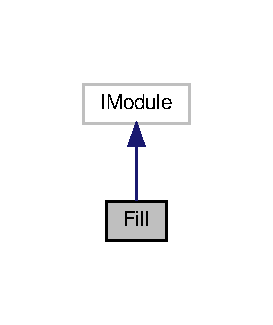
\includegraphics[width=131pt]{class_fill__inherit__graph}
\end{center}
\end{figure}


Collaboration diagram for Fill\+:\nopagebreak
\begin{figure}[H]
\begin{center}
\leavevmode
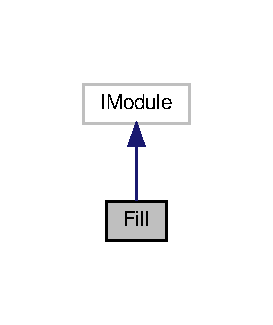
\includegraphics[width=131pt]{class_fill__coll__graph}
\end{center}
\end{figure}
\subsection*{Public Member Functions}
\begin{DoxyCompactItemize}
\item 
\hyperlink{class_fill_a686b6c06d79a3e7272cc400f29aa7e44}{Fill} ()=default
\begin{DoxyCompactList}\small\item\em Default constructor for the fill module. \end{DoxyCompactList}\item 
virtual const char $\ast$ \hyperlink{class_fill_a5116eca7a853356f420f6474ade0983b}{get\+Name} (void) const
\begin{DoxyCompactList}\small\item\em Get the name of the module. \end{DoxyCompactList}\item 
virtual void \hyperlink{class_fill_a440901ea6a6270194ca7e0e19c9bd88e}{on\+Register\+Callbacks} (o\+Z\+::\+Pipeline \&pipeline)
\begin{DoxyCompactList}\small\item\em Fct for the pipeline (load in the right place in the right position) \end{DoxyCompactList}\end{DoxyCompactItemize}


\subsection{Detailed Description}
\hyperlink{class_fill}{Fill} class to manage the \hyperlink{class_fill}{Fill} module. 

Definition at line 20 of file Fill\+Page.\+hpp.



\subsection{Constructor \& Destructor Documentation}
\mbox{\Hypertarget{class_fill_a686b6c06d79a3e7272cc400f29aa7e44}\label{class_fill_a686b6c06d79a3e7272cc400f29aa7e44}} 
\index{Fill@{Fill}!Fill@{Fill}}
\index{Fill@{Fill}!Fill@{Fill}}
\subsubsection{\texorpdfstring{Fill()}{Fill()}}
{\footnotesize\ttfamily Fill\+::\+Fill (\begin{DoxyParamCaption}{ }\end{DoxyParamCaption})\hspace{0.3cm}{\ttfamily [default]}}



Default constructor for the fill module. 



\subsection{Member Function Documentation}
\mbox{\Hypertarget{class_fill_a5116eca7a853356f420f6474ade0983b}\label{class_fill_a5116eca7a853356f420f6474ade0983b}} 
\index{Fill@{Fill}!get\+Name@{get\+Name}}
\index{get\+Name@{get\+Name}!Fill@{Fill}}
\subsubsection{\texorpdfstring{get\+Name()}{getName()}}
{\footnotesize\ttfamily virtual const char$\ast$ Fill\+::get\+Name (\begin{DoxyParamCaption}\item[{void}]{ }\end{DoxyParamCaption}) const\hspace{0.3cm}{\ttfamily [inline]}, {\ttfamily [virtual]}}



Get the name of the module. 

\begin{DoxyReturn}{Returns}
The name of the module 
\end{DoxyReturn}


Definition at line 32 of file Fill\+Page.\+hpp.

\mbox{\Hypertarget{class_fill_a440901ea6a6270194ca7e0e19c9bd88e}\label{class_fill_a440901ea6a6270194ca7e0e19c9bd88e}} 
\index{Fill@{Fill}!on\+Register\+Callbacks@{on\+Register\+Callbacks}}
\index{on\+Register\+Callbacks@{on\+Register\+Callbacks}!Fill@{Fill}}
\subsubsection{\texorpdfstring{on\+Register\+Callbacks()}{onRegisterCallbacks()}}
{\footnotesize\ttfamily void Fill\+::on\+Register\+Callbacks (\begin{DoxyParamCaption}\item[{o\+Z\+::\+Pipeline \&}]{pipeline }\end{DoxyParamCaption})\hspace{0.3cm}{\ttfamily [virtual]}}



Fct for the pipeline (load in the right place in the right position) 


\begin{DoxyParams}{Parameters}
{\em pipeline} & Reference on the pipeline where the module is load \\
\hline
\end{DoxyParams}


Definition at line 17 of file Fill\+Page.\+cpp.



The documentation for this class was generated from the following files\+:\begin{DoxyCompactItemize}
\item 
src/modules/fill\+Page/\hyperlink{_fill_page_8hpp}{Fill\+Page.\+hpp}\item 
src/modules/fill\+Page/\hyperlink{_fill_page_8cpp}{Fill\+Page.\+cpp}\end{DoxyCompactItemize}

\hypertarget{classtls_1_1_json_loader}{}\section{tls\+:\+:Json\+Loader Class Reference}
\label{classtls_1_1_json_loader}\index{tls\+::\+Json\+Loader@{tls\+::\+Json\+Loader}}


\hyperlink{classtls_1_1_json_loader}{Json\+Loader} class to manage a json file.  




{\ttfamily \#include $<$Json\+Loader.\+hpp$>$}

\subsection*{Public Member Functions}
\begin{DoxyCompactItemize}
\item 
\hyperlink{classtls_1_1_json_loader_a9f9fc1f46e82b4f377b22c8acf0f3b9d}{Json\+Loader} ()
\begin{DoxyCompactList}\small\item\em Construct a new \hyperlink{classtls_1_1_json_loader}{Json\+Loader} object. \end{DoxyCompactList}\item 
\hyperlink{classtls_1_1_json_loader_ad6ec799a31fbae8ea01a9d6c278ad6e3}{Json\+Loader} (const std\+::filesystem\+::path \&path)
\begin{DoxyCompactList}\small\item\em Construct a new \hyperlink{classtls_1_1_json_loader}{Json\+Loader} object. \end{DoxyCompactList}\item 
\hyperlink{classtls_1_1_json_loader_a0826d5c9480c38d010fe580101d916e0}{Json\+Loader} (const \hyperlink{namespacetls_a4e8d32383e204ee25990db65651ea712}{json} \&object)
\begin{DoxyCompactList}\small\item\em Construct a new \hyperlink{classtls_1_1_json_loader}{Json\+Loader} object. \end{DoxyCompactList}\item 
\hyperlink{classtls_1_1_json_loader_a2d493a7049c70e6974a3daf2ef2e71f9}{$\sim$\+Json\+Loader} ()=default
\begin{DoxyCompactList}\small\item\em Destroy the \hyperlink{classtls_1_1_json_loader}{Json\+Loader} object. \end{DoxyCompactList}\item 
void \hyperlink{classtls_1_1_json_loader_ad587735dbb8e8cfc5cd002a0aa9a7d7f}{load} (const std\+::filesystem\+::path \&path)
\begin{DoxyCompactList}\small\item\em Load a json from a given json file. \end{DoxyCompactList}\item 
const \hyperlink{namespacetls_a4e8d32383e204ee25990db65651ea712}{json} \hyperlink{classtls_1_1_json_loader_a0174b44e635a44811616c394d89b73e5}{get} (const std\+::string \&to\+\_\+get) const
\begin{DoxyCompactList}\small\item\em Get data from the json previously loaded. \end{DoxyCompactList}\item 
const \hyperlink{namespacetls_a4e8d32383e204ee25990db65651ea712}{json} \hyperlink{classtls_1_1_json_loader_aef4c88eb0589673f806e7fedf7b3b6b9}{get\+Json} () const noexcept
\begin{DoxyCompactList}\small\item\em Get all json file content deserialized. \end{DoxyCompactList}\item 
const bool \hyperlink{classtls_1_1_json_loader_ac7fa5168de0714b4ab4cf3f7f366dbdf}{has\+Loaded} () const noexcept
\begin{DoxyCompactList}\small\item\em Check if a json file has already been loaded. \end{DoxyCompactList}\end{DoxyCompactItemize}


\subsection{Detailed Description}
\hyperlink{classtls_1_1_json_loader}{Json\+Loader} class to manage a json file. 

Definition at line 25 of file Json\+Loader.\+hpp.



\subsection{Constructor \& Destructor Documentation}
\mbox{\Hypertarget{classtls_1_1_json_loader_a9f9fc1f46e82b4f377b22c8acf0f3b9d}\label{classtls_1_1_json_loader_a9f9fc1f46e82b4f377b22c8acf0f3b9d}} 
\index{tls\+::\+Json\+Loader@{tls\+::\+Json\+Loader}!Json\+Loader@{Json\+Loader}}
\index{Json\+Loader@{Json\+Loader}!tls\+::\+Json\+Loader@{tls\+::\+Json\+Loader}}
\subsubsection{\texorpdfstring{Json\+Loader()}{JsonLoader()}\hspace{0.1cm}{\footnotesize\ttfamily [1/3]}}
{\footnotesize\ttfamily Json\+Loader\+::\+Json\+Loader (\begin{DoxyParamCaption}{ }\end{DoxyParamCaption})}



Construct a new \hyperlink{classtls_1_1_json_loader}{Json\+Loader} object. 



Definition at line 12 of file Json\+Loader.\+cpp.

\mbox{\Hypertarget{classtls_1_1_json_loader_ad6ec799a31fbae8ea01a9d6c278ad6e3}\label{classtls_1_1_json_loader_ad6ec799a31fbae8ea01a9d6c278ad6e3}} 
\index{tls\+::\+Json\+Loader@{tls\+::\+Json\+Loader}!Json\+Loader@{Json\+Loader}}
\index{Json\+Loader@{Json\+Loader}!tls\+::\+Json\+Loader@{tls\+::\+Json\+Loader}}
\subsubsection{\texorpdfstring{Json\+Loader()}{JsonLoader()}\hspace{0.1cm}{\footnotesize\ttfamily [2/3]}}
{\footnotesize\ttfamily Json\+Loader\+::\+Json\+Loader (\begin{DoxyParamCaption}\item[{const std\+::filesystem\+::path \&}]{path }\end{DoxyParamCaption})}



Construct a new \hyperlink{classtls_1_1_json_loader}{Json\+Loader} object. 


\begin{DoxyParams}{Parameters}
{\em path} & Path of the json file to load. \\
\hline
\end{DoxyParams}


Definition at line 17 of file Json\+Loader.\+cpp.

\mbox{\Hypertarget{classtls_1_1_json_loader_a0826d5c9480c38d010fe580101d916e0}\label{classtls_1_1_json_loader_a0826d5c9480c38d010fe580101d916e0}} 
\index{tls\+::\+Json\+Loader@{tls\+::\+Json\+Loader}!Json\+Loader@{Json\+Loader}}
\index{Json\+Loader@{Json\+Loader}!tls\+::\+Json\+Loader@{tls\+::\+Json\+Loader}}
\subsubsection{\texorpdfstring{Json\+Loader()}{JsonLoader()}\hspace{0.1cm}{\footnotesize\ttfamily [3/3]}}
{\footnotesize\ttfamily Json\+Loader\+::\+Json\+Loader (\begin{DoxyParamCaption}\item[{const \hyperlink{namespacetls_a4e8d32383e204ee25990db65651ea712}{json} \&}]{object }\end{DoxyParamCaption})}



Construct a new \hyperlink{classtls_1_1_json_loader}{Json\+Loader} object. 


\begin{DoxyParams}{Parameters}
{\em object} & Json object to load. \\
\hline
\end{DoxyParams}


Definition at line 23 of file Json\+Loader.\+cpp.

\mbox{\Hypertarget{classtls_1_1_json_loader_a2d493a7049c70e6974a3daf2ef2e71f9}\label{classtls_1_1_json_loader_a2d493a7049c70e6974a3daf2ef2e71f9}} 
\index{tls\+::\+Json\+Loader@{tls\+::\+Json\+Loader}!````~Json\+Loader@{$\sim$\+Json\+Loader}}
\index{````~Json\+Loader@{$\sim$\+Json\+Loader}!tls\+::\+Json\+Loader@{tls\+::\+Json\+Loader}}
\subsubsection{\texorpdfstring{$\sim$\+Json\+Loader()}{~JsonLoader()}}
{\footnotesize\ttfamily tls\+::\+Json\+Loader\+::$\sim$\+Json\+Loader (\begin{DoxyParamCaption}{ }\end{DoxyParamCaption})\hspace{0.3cm}{\ttfamily [default]}}



Destroy the \hyperlink{classtls_1_1_json_loader}{Json\+Loader} object. 



\subsection{Member Function Documentation}
\mbox{\Hypertarget{classtls_1_1_json_loader_a0174b44e635a44811616c394d89b73e5}\label{classtls_1_1_json_loader_a0174b44e635a44811616c394d89b73e5}} 
\index{tls\+::\+Json\+Loader@{tls\+::\+Json\+Loader}!get@{get}}
\index{get@{get}!tls\+::\+Json\+Loader@{tls\+::\+Json\+Loader}}
\subsubsection{\texorpdfstring{get()}{get()}}
{\footnotesize\ttfamily const \hyperlink{namespacetls_a4e8d32383e204ee25990db65651ea712}{json} Json\+Loader\+::get (\begin{DoxyParamCaption}\item[{const std\+::string \&}]{to\+\_\+get }\end{DoxyParamCaption}) const}



Get data from the json previously loaded. 


\begin{DoxyParams}{Parameters}
{\em to\+\_\+get} & Data key in the json.\\
\hline
\end{DoxyParams}
\begin{DoxyReturn}{Returns}
Data if found otherwise null json object. 
\end{DoxyReturn}


Definition at line 37 of file Json\+Loader.\+cpp.

\mbox{\Hypertarget{classtls_1_1_json_loader_aef4c88eb0589673f806e7fedf7b3b6b9}\label{classtls_1_1_json_loader_aef4c88eb0589673f806e7fedf7b3b6b9}} 
\index{tls\+::\+Json\+Loader@{tls\+::\+Json\+Loader}!get\+Json@{get\+Json}}
\index{get\+Json@{get\+Json}!tls\+::\+Json\+Loader@{tls\+::\+Json\+Loader}}
\subsubsection{\texorpdfstring{get\+Json()}{getJson()}}
{\footnotesize\ttfamily const \hyperlink{namespacetls_a4e8d32383e204ee25990db65651ea712}{json} Json\+Loader\+::get\+Json (\begin{DoxyParamCaption}{ }\end{DoxyParamCaption}) const\hspace{0.3cm}{\ttfamily [noexcept]}}



Get all json file content deserialized. 

\begin{DoxyReturn}{Returns}
Json object. 
\end{DoxyReturn}


Definition at line 49 of file Json\+Loader.\+cpp.

\mbox{\Hypertarget{classtls_1_1_json_loader_ac7fa5168de0714b4ab4cf3f7f366dbdf}\label{classtls_1_1_json_loader_ac7fa5168de0714b4ab4cf3f7f366dbdf}} 
\index{tls\+::\+Json\+Loader@{tls\+::\+Json\+Loader}!has\+Loaded@{has\+Loaded}}
\index{has\+Loaded@{has\+Loaded}!tls\+::\+Json\+Loader@{tls\+::\+Json\+Loader}}
\subsubsection{\texorpdfstring{has\+Loaded()}{hasLoaded()}}
{\footnotesize\ttfamily const bool Json\+Loader\+::has\+Loaded (\begin{DoxyParamCaption}{ }\end{DoxyParamCaption}) const\hspace{0.3cm}{\ttfamily [noexcept]}}



Check if a json file has already been loaded. 

\begin{DoxyReturn}{Returns}
True if a file has been loaded otherwise false. 
\end{DoxyReturn}


Definition at line 54 of file Json\+Loader.\+cpp.

\mbox{\Hypertarget{classtls_1_1_json_loader_ad587735dbb8e8cfc5cd002a0aa9a7d7f}\label{classtls_1_1_json_loader_ad587735dbb8e8cfc5cd002a0aa9a7d7f}} 
\index{tls\+::\+Json\+Loader@{tls\+::\+Json\+Loader}!load@{load}}
\index{load@{load}!tls\+::\+Json\+Loader@{tls\+::\+Json\+Loader}}
\subsubsection{\texorpdfstring{load()}{load()}}
{\footnotesize\ttfamily void Json\+Loader\+::load (\begin{DoxyParamCaption}\item[{const std\+::filesystem\+::path \&}]{path }\end{DoxyParamCaption})}



Load a json from a given json file. 


\begin{DoxyParams}{Parameters}
{\em path} & Path of the json file to load. \\
\hline
\end{DoxyParams}


Definition at line 29 of file Json\+Loader.\+cpp.



The documentation for this class was generated from the following files\+:\begin{DoxyCompactItemize}
\item 
src/utils/\hyperlink{_json_loader_8hpp}{Json\+Loader.\+hpp}\item 
src/utils/\hyperlink{_json_loader_8cpp}{Json\+Loader.\+cpp}\end{DoxyCompactItemize}

\hypertarget{class_zia_1_1_log}{}\section{Zia\+:\+:Log Class Reference}
\label{class_zia_1_1_log}\index{Zia\+::\+Log@{Zia\+::\+Log}}


\hyperlink{class_zia_1_1_log}{Log} class to manage the log.  




{\ttfamily \#include $<$Log.\+hpp$>$}

\subsection*{Static Public Member Functions}
\begin{DoxyCompactItemize}
\item 
static void \hyperlink{class_zia_1_1_log_ae26eb7733ba9cda16a36d2ad25c93bd4}{set\+Path\+File} (const std\+::string \&) noexcept
\item 
static void \hyperlink{class_zia_1_1_log_a7abad30f76aea6c210ae245885f05137}{info} (const std\+::string \&msg, bool write\+In\+File=false) noexcept
\item 
static void \hyperlink{class_zia_1_1_log_a4522d6218b4fb537c4291c36c171a855}{warning} (const std\+::string \&msg, bool write\+In\+File=false) noexcept
\item 
static void \hyperlink{class_zia_1_1_log_a5a7899f592f85e1da39e90ba32eef98b}{critical} (const std\+::string \&msg, bool write\+In\+File=false) noexcept
\end{DoxyCompactItemize}
\subsection*{Static Public Attributes}
\begin{DoxyCompactItemize}
\item 
static long \hyperlink{class_zia_1_1_log_a3080034dce1aca8c3cc7b85775d30a1b}{Numbers\+Info} = 0
\item 
static long \hyperlink{class_zia_1_1_log_a64ce5169f6328628c8074a7664f8445c}{Numbers\+Warning} = 0
\item 
static long \hyperlink{class_zia_1_1_log_ada4fab060168cbb9504c7ffa4b762868}{Numbers\+Critical} = 0
\end{DoxyCompactItemize}


\subsection{Detailed Description}
\hyperlink{class_zia_1_1_log}{Log} class to manage the log. 

Definition at line 20 of file Log.\+hpp.



\subsection{Member Function Documentation}
\mbox{\Hypertarget{class_zia_1_1_log_a5a7899f592f85e1da39e90ba32eef98b}\label{class_zia_1_1_log_a5a7899f592f85e1da39e90ba32eef98b}} 
\index{Zia\+::\+Log@{Zia\+::\+Log}!critical@{critical}}
\index{critical@{critical}!Zia\+::\+Log@{Zia\+::\+Log}}
\subsubsection{\texorpdfstring{critical()}{critical()}}
{\footnotesize\ttfamily void Zia\+::\+Log\+::critical (\begin{DoxyParamCaption}\item[{const std\+::string \&}]{msg,  }\item[{bool}]{write\+In\+File = {\ttfamily false} }\end{DoxyParamCaption})\hspace{0.3cm}{\ttfamily [static]}, {\ttfamily [noexcept]}}



Definition at line 35 of file Log.\+cpp.

\mbox{\Hypertarget{class_zia_1_1_log_a7abad30f76aea6c210ae245885f05137}\label{class_zia_1_1_log_a7abad30f76aea6c210ae245885f05137}} 
\index{Zia\+::\+Log@{Zia\+::\+Log}!info@{info}}
\index{info@{info}!Zia\+::\+Log@{Zia\+::\+Log}}
\subsubsection{\texorpdfstring{info()}{info()}}
{\footnotesize\ttfamily void Zia\+::\+Log\+::info (\begin{DoxyParamCaption}\item[{const std\+::string \&}]{msg,  }\item[{bool}]{write\+In\+File = {\ttfamily false} }\end{DoxyParamCaption})\hspace{0.3cm}{\ttfamily [static]}, {\ttfamily [noexcept]}}



Definition at line 21 of file Log.\+cpp.

\mbox{\Hypertarget{class_zia_1_1_log_ae26eb7733ba9cda16a36d2ad25c93bd4}\label{class_zia_1_1_log_ae26eb7733ba9cda16a36d2ad25c93bd4}} 
\index{Zia\+::\+Log@{Zia\+::\+Log}!set\+Path\+File@{set\+Path\+File}}
\index{set\+Path\+File@{set\+Path\+File}!Zia\+::\+Log@{Zia\+::\+Log}}
\subsubsection{\texorpdfstring{set\+Path\+File()}{setPathFile()}}
{\footnotesize\ttfamily void Zia\+::\+Log\+::set\+Path\+File (\begin{DoxyParamCaption}\item[{const std\+::string \&}]{path }\end{DoxyParamCaption})\hspace{0.3cm}{\ttfamily [static]}, {\ttfamily [noexcept]}}



Definition at line 16 of file Log.\+cpp.

\mbox{\Hypertarget{class_zia_1_1_log_a4522d6218b4fb537c4291c36c171a855}\label{class_zia_1_1_log_a4522d6218b4fb537c4291c36c171a855}} 
\index{Zia\+::\+Log@{Zia\+::\+Log}!warning@{warning}}
\index{warning@{warning}!Zia\+::\+Log@{Zia\+::\+Log}}
\subsubsection{\texorpdfstring{warning()}{warning()}}
{\footnotesize\ttfamily void Zia\+::\+Log\+::warning (\begin{DoxyParamCaption}\item[{const std\+::string \&}]{msg,  }\item[{bool}]{write\+In\+File = {\ttfamily false} }\end{DoxyParamCaption})\hspace{0.3cm}{\ttfamily [static]}, {\ttfamily [noexcept]}}



Definition at line 28 of file Log.\+cpp.



\subsection{Member Data Documentation}
\mbox{\Hypertarget{class_zia_1_1_log_ada4fab060168cbb9504c7ffa4b762868}\label{class_zia_1_1_log_ada4fab060168cbb9504c7ffa4b762868}} 
\index{Zia\+::\+Log@{Zia\+::\+Log}!Numbers\+Critical@{Numbers\+Critical}}
\index{Numbers\+Critical@{Numbers\+Critical}!Zia\+::\+Log@{Zia\+::\+Log}}
\subsubsection{\texorpdfstring{Numbers\+Critical}{NumbersCritical}}
{\footnotesize\ttfamily long Zia\+::\+Log\+::\+Numbers\+Critical = 0\hspace{0.3cm}{\ttfamily [static]}}



Definition at line 30 of file Log.\+hpp.

\mbox{\Hypertarget{class_zia_1_1_log_a3080034dce1aca8c3cc7b85775d30a1b}\label{class_zia_1_1_log_a3080034dce1aca8c3cc7b85775d30a1b}} 
\index{Zia\+::\+Log@{Zia\+::\+Log}!Numbers\+Info@{Numbers\+Info}}
\index{Numbers\+Info@{Numbers\+Info}!Zia\+::\+Log@{Zia\+::\+Log}}
\subsubsection{\texorpdfstring{Numbers\+Info}{NumbersInfo}}
{\footnotesize\ttfamily long Zia\+::\+Log\+::\+Numbers\+Info = 0\hspace{0.3cm}{\ttfamily [static]}}



Definition at line 28 of file Log.\+hpp.

\mbox{\Hypertarget{class_zia_1_1_log_a64ce5169f6328628c8074a7664f8445c}\label{class_zia_1_1_log_a64ce5169f6328628c8074a7664f8445c}} 
\index{Zia\+::\+Log@{Zia\+::\+Log}!Numbers\+Warning@{Numbers\+Warning}}
\index{Numbers\+Warning@{Numbers\+Warning}!Zia\+::\+Log@{Zia\+::\+Log}}
\subsubsection{\texorpdfstring{Numbers\+Warning}{NumbersWarning}}
{\footnotesize\ttfamily long Zia\+::\+Log\+::\+Numbers\+Warning = 0\hspace{0.3cm}{\ttfamily [static]}}



Definition at line 29 of file Log.\+hpp.



The documentation for this class was generated from the following files\+:\begin{DoxyCompactItemize}
\item 
src/server/\hyperlink{_log_8hpp}{Log.\+hpp}\item 
src/server/\hyperlink{_log_8cpp}{Log.\+cpp}\end{DoxyCompactItemize}

\hypertarget{class_zia_1_1_module}{}\section{Zia\+:\+:Module Class Reference}
\label{class_zia_1_1_module}\index{Zia\+::\+Module@{Zia\+::\+Module}}


\hyperlink{class_zia_1_1_module}{Module} class to manage the modules.  




{\ttfamily \#include $<$Module.\+hpp$>$}

\subsection*{Public Member Functions}
\begin{DoxyCompactItemize}
\item 
\hyperlink{class_zia_1_1_module_a4e5330e20703c939d940afe737bd4d1b}{Module} (const \hyperlink{namespacecfg_af0aed6e47bd26e91ad7d69467f96caaf}{cfg\+::\+File\+Descriptor} \&path)
\begin{DoxyCompactList}\small\item\em Construct a new \hyperlink{class_zia_1_1_module}{Module} object. \end{DoxyCompactList}\item 
\hyperlink{class_zia_1_1_module_a91f712e682b2b949656b90796879d8b1}{$\sim$\+Module} ()=default
\begin{DoxyCompactList}\small\item\em Destroy the \hyperlink{class_zia_1_1_module}{Module} object. \end{DoxyCompactList}\item 
const std\+::string \hyperlink{class_zia_1_1_module_ac0eaf9796e9cb65c279743f3c6377b1b}{get\+Name} () const noexcept
\begin{DoxyCompactList}\small\item\em Get the module\textquotesingle{}s name. \end{DoxyCompactList}\item 
const std\+::string \hyperlink{class_zia_1_1_module_a93f4a37a5e91739c2584292e540d6dff}{get\+Name} (const \hyperlink{namespacecfg_af0aed6e47bd26e91ad7d69467f96caaf}{cfg\+::\+File\+Descriptor} \&file) const
\begin{DoxyCompactList}\small\item\em Generate the module\textquotesingle{}s name from a file descriptor. \end{DoxyCompactList}\item 
const std\+::string \hyperlink{class_zia_1_1_module_ae9e284d2b324100926271ca383704552}{get\+Path} () const noexcept
\begin{DoxyCompactList}\small\item\em Get the module\textquotesingle{}s library path. \end{DoxyCompactList}\end{DoxyCompactItemize}


\subsection{Detailed Description}
\hyperlink{class_zia_1_1_module}{Module} class to manage the modules. 

Definition at line 17 of file Module.\+hpp.



\subsection{Constructor \& Destructor Documentation}
\mbox{\Hypertarget{class_zia_1_1_module_a4e5330e20703c939d940afe737bd4d1b}\label{class_zia_1_1_module_a4e5330e20703c939d940afe737bd4d1b}} 
\index{Zia\+::\+Module@{Zia\+::\+Module}!Module@{Module}}
\index{Module@{Module}!Zia\+::\+Module@{Zia\+::\+Module}}
\subsubsection{\texorpdfstring{Module()}{Module()}}
{\footnotesize\ttfamily Module\+::\+Module (\begin{DoxyParamCaption}\item[{const \hyperlink{namespacecfg_af0aed6e47bd26e91ad7d69467f96caaf}{cfg\+::\+File\+Descriptor} \&}]{path }\end{DoxyParamCaption})}



Construct a new \hyperlink{class_zia_1_1_module}{Module} object. 


\begin{DoxyParams}{Parameters}
{\em path} & File descriptor of the module library. \\
\hline
\end{DoxyParams}


Definition at line 12 of file Module.\+cpp.

\mbox{\Hypertarget{class_zia_1_1_module_a91f712e682b2b949656b90796879d8b1}\label{class_zia_1_1_module_a91f712e682b2b949656b90796879d8b1}} 
\index{Zia\+::\+Module@{Zia\+::\+Module}!````~Module@{$\sim$\+Module}}
\index{````~Module@{$\sim$\+Module}!Zia\+::\+Module@{Zia\+::\+Module}}
\subsubsection{\texorpdfstring{$\sim$\+Module()}{~Module()}}
{\footnotesize\ttfamily Zia\+::\+Module\+::$\sim$\+Module (\begin{DoxyParamCaption}{ }\end{DoxyParamCaption})\hspace{0.3cm}{\ttfamily [default]}}



Destroy the \hyperlink{class_zia_1_1_module}{Module} object. 



\subsection{Member Function Documentation}
\mbox{\Hypertarget{class_zia_1_1_module_ac0eaf9796e9cb65c279743f3c6377b1b}\label{class_zia_1_1_module_ac0eaf9796e9cb65c279743f3c6377b1b}} 
\index{Zia\+::\+Module@{Zia\+::\+Module}!get\+Name@{get\+Name}}
\index{get\+Name@{get\+Name}!Zia\+::\+Module@{Zia\+::\+Module}}
\subsubsection{\texorpdfstring{get\+Name()}{getName()}\hspace{0.1cm}{\footnotesize\ttfamily [1/2]}}
{\footnotesize\ttfamily const std\+::string Module\+::get\+Name (\begin{DoxyParamCaption}\item[{void}]{ }\end{DoxyParamCaption}) const\hspace{0.3cm}{\ttfamily [noexcept]}}



Get the module\textquotesingle{}s name. 

\begin{DoxyReturn}{Returns}
\hyperlink{class_zia_1_1_module}{Module}\textquotesingle{}s name. 
\end{DoxyReturn}


Definition at line 18 of file Module.\+cpp.

\mbox{\Hypertarget{class_zia_1_1_module_a93f4a37a5e91739c2584292e540d6dff}\label{class_zia_1_1_module_a93f4a37a5e91739c2584292e540d6dff}} 
\index{Zia\+::\+Module@{Zia\+::\+Module}!get\+Name@{get\+Name}}
\index{get\+Name@{get\+Name}!Zia\+::\+Module@{Zia\+::\+Module}}
\subsubsection{\texorpdfstring{get\+Name()}{getName()}\hspace{0.1cm}{\footnotesize\ttfamily [2/2]}}
{\footnotesize\ttfamily const std\+::string Module\+::get\+Name (\begin{DoxyParamCaption}\item[{const \hyperlink{namespacecfg_af0aed6e47bd26e91ad7d69467f96caaf}{cfg\+::\+File\+Descriptor} \&}]{file }\end{DoxyParamCaption}) const}



Generate the module\textquotesingle{}s name from a file descriptor. 

\begin{DoxyReturn}{Returns}
Generated module name. 
\end{DoxyReturn}


Definition at line 23 of file Module.\+cpp.

\mbox{\Hypertarget{class_zia_1_1_module_ae9e284d2b324100926271ca383704552}\label{class_zia_1_1_module_ae9e284d2b324100926271ca383704552}} 
\index{Zia\+::\+Module@{Zia\+::\+Module}!get\+Path@{get\+Path}}
\index{get\+Path@{get\+Path}!Zia\+::\+Module@{Zia\+::\+Module}}
\subsubsection{\texorpdfstring{get\+Path()}{getPath()}}
{\footnotesize\ttfamily const std\+::string Module\+::get\+Path (\begin{DoxyParamCaption}{ }\end{DoxyParamCaption}) const\hspace{0.3cm}{\ttfamily [noexcept]}}



Get the module\textquotesingle{}s library path. 

\begin{DoxyReturn}{Returns}
\hyperlink{class_zia_1_1_module}{Module}\textquotesingle{}s library path. 
\end{DoxyReturn}


Definition at line 33 of file Module.\+cpp.



The documentation for this class was generated from the following files\+:\begin{DoxyCompactItemize}
\item 
src/server/\hyperlink{_module_8hpp}{Module.\+hpp}\item 
src/server/\hyperlink{_module_8cpp}{Module.\+cpp}\end{DoxyCompactItemize}

\hypertarget{class_parser}{}\section{Parser Class Reference}
\label{class_parser}\index{Parser@{Parser}}


\hyperlink{class_parser}{Parser} class to manage the parser module.  




{\ttfamily \#include $<$Parser\+Module.\+hpp$>$}



Inheritance diagram for Parser\+:\nopagebreak
\begin{figure}[H]
\begin{center}
\leavevmode
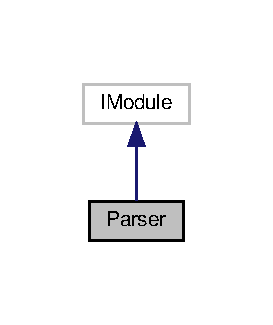
\includegraphics[width=131pt]{class_parser__inherit__graph}
\end{center}
\end{figure}


Collaboration diagram for Parser\+:\nopagebreak
\begin{figure}[H]
\begin{center}
\leavevmode
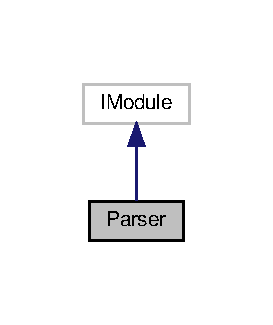
\includegraphics[width=131pt]{class_parser__coll__graph}
\end{center}
\end{figure}
\subsection*{Public Member Functions}
\begin{DoxyCompactItemize}
\item 
\hyperlink{class_parser_a5208129b497bfdf7c8ecceeb70e4bba8}{Parser} ()=default
\begin{DoxyCompactList}\small\item\em Default constructor for the parset module. \end{DoxyCompactList}\item 
virtual const char $\ast$ \hyperlink{class_parser_a655ca8534272a48ee94113695f6494fc}{get\+Name} (void) const
\begin{DoxyCompactList}\small\item\em Get the name of the module. \end{DoxyCompactList}\item 
virtual void \hyperlink{class_parser_a0e8278ef45fabe33144c78c51fbfcf7d}{on\+Register\+Callbacks} (o\+Z\+::\+Pipeline \&pipeline)
\begin{DoxyCompactList}\small\item\em Fct for the pipeline (load in the right place in the right position) \end{DoxyCompactList}\end{DoxyCompactItemize}


\subsection{Detailed Description}
\hyperlink{class_parser}{Parser} class to manage the parser module. 

Definition at line 48 of file Parser\+Module.\+hpp.



\subsection{Constructor \& Destructor Documentation}
\mbox{\Hypertarget{class_parser_a5208129b497bfdf7c8ecceeb70e4bba8}\label{class_parser_a5208129b497bfdf7c8ecceeb70e4bba8}} 
\index{Parser@{Parser}!Parser@{Parser}}
\index{Parser@{Parser}!Parser@{Parser}}
\subsubsection{\texorpdfstring{Parser()}{Parser()}}
{\footnotesize\ttfamily Parser\+::\+Parser (\begin{DoxyParamCaption}{ }\end{DoxyParamCaption})\hspace{0.3cm}{\ttfamily [default]}}



Default constructor for the parset module. 



\subsection{Member Function Documentation}
\mbox{\Hypertarget{class_parser_a655ca8534272a48ee94113695f6494fc}\label{class_parser_a655ca8534272a48ee94113695f6494fc}} 
\index{Parser@{Parser}!get\+Name@{get\+Name}}
\index{get\+Name@{get\+Name}!Parser@{Parser}}
\subsubsection{\texorpdfstring{get\+Name()}{getName()}}
{\footnotesize\ttfamily virtual const char$\ast$ Parser\+::get\+Name (\begin{DoxyParamCaption}\item[{void}]{ }\end{DoxyParamCaption}) const\hspace{0.3cm}{\ttfamily [inline]}, {\ttfamily [virtual]}}



Get the name of the module. 

\begin{DoxyReturn}{Returns}
The name of the module 
\end{DoxyReturn}


Definition at line 60 of file Parser\+Module.\+hpp.

\mbox{\Hypertarget{class_parser_a0e8278ef45fabe33144c78c51fbfcf7d}\label{class_parser_a0e8278ef45fabe33144c78c51fbfcf7d}} 
\index{Parser@{Parser}!on\+Register\+Callbacks@{on\+Register\+Callbacks}}
\index{on\+Register\+Callbacks@{on\+Register\+Callbacks}!Parser@{Parser}}
\subsubsection{\texorpdfstring{on\+Register\+Callbacks()}{onRegisterCallbacks()}}
{\footnotesize\ttfamily void Parser\+::on\+Register\+Callbacks (\begin{DoxyParamCaption}\item[{o\+Z\+::\+Pipeline \&}]{pipeline }\end{DoxyParamCaption})\hspace{0.3cm}{\ttfamily [virtual]}}



Fct for the pipeline (load in the right place in the right position) 


\begin{DoxyParams}{Parameters}
{\em pipeline} & Reference on the pipeline where the module is load \\
\hline
\end{DoxyParams}


Definition at line 15 of file Parser\+Module.\+cpp.



The documentation for this class was generated from the following files\+:\begin{DoxyCompactItemize}
\item 
src/modules/parser/\hyperlink{_parser_module_8hpp}{Parser\+Module.\+hpp}\item 
src/modules/parser/\hyperlink{_parser_module_8cpp}{Parser\+Module.\+cpp}\end{DoxyCompactItemize}

\hypertarget{class_p_h_p___c_g_i}{}\section{P\+H\+P\+\_\+\+C\+GI Class Reference}
\label{class_p_h_p___c_g_i}\index{P\+H\+P\+\_\+\+C\+GI@{P\+H\+P\+\_\+\+C\+GI}}


\hyperlink{class_p_h_p___c_g_i}{P\+H\+P\+\_\+\+C\+GI} class to manage the P\+HP module.  




{\ttfamily \#include $<$P\+H\+P\+Module.\+hpp$>$}



Inheritance diagram for P\+H\+P\+\_\+\+C\+GI\+:\nopagebreak
\begin{figure}[H]
\begin{center}
\leavevmode
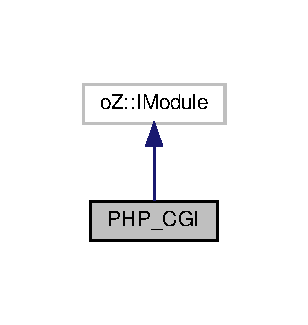
\includegraphics[width=148pt]{class_p_h_p___c_g_i__inherit__graph}
\end{center}
\end{figure}


Collaboration diagram for P\+H\+P\+\_\+\+C\+GI\+:\nopagebreak
\begin{figure}[H]
\begin{center}
\leavevmode
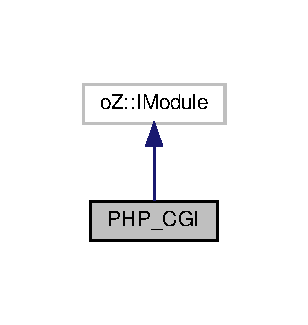
\includegraphics[width=148pt]{class_p_h_p___c_g_i__coll__graph}
\end{center}
\end{figure}
\subsection*{Public Member Functions}
\begin{DoxyCompactItemize}
\item 
\hyperlink{class_p_h_p___c_g_i_a4ce89837013dbd5836475cbded08dee7}{P\+H\+P\+\_\+\+C\+GI} ()=default
\begin{DoxyCompactList}\small\item\em Default constructor for the php module. \end{DoxyCompactList}\item 
virtual const char $\ast$ \hyperlink{class_p_h_p___c_g_i_a6446691803801b4100f18bcd53899237}{get\+Name} (void) const
\begin{DoxyCompactList}\small\item\em Get the name of the module. \end{DoxyCompactList}\item 
virtual void \hyperlink{class_p_h_p___c_g_i_a5f85735822d4cb288b34182d43b2d059}{on\+Register\+Callbacks} (o\+Z\+::\+Pipeline \&pipeline)
\begin{DoxyCompactList}\small\item\em Fct for the pipeline (load in the right place in the right position) \end{DoxyCompactList}\end{DoxyCompactItemize}


\subsection{Detailed Description}
\hyperlink{class_p_h_p___c_g_i}{P\+H\+P\+\_\+\+C\+GI} class to manage the P\+HP module. 

Definition at line 40 of file P\+H\+P\+Module.\+hpp.



\subsection{Constructor \& Destructor Documentation}
\mbox{\Hypertarget{class_p_h_p___c_g_i_a4ce89837013dbd5836475cbded08dee7}\label{class_p_h_p___c_g_i_a4ce89837013dbd5836475cbded08dee7}} 
\index{P\+H\+P\+\_\+\+C\+GI@{P\+H\+P\+\_\+\+C\+GI}!P\+H\+P\+\_\+\+C\+GI@{P\+H\+P\+\_\+\+C\+GI}}
\index{P\+H\+P\+\_\+\+C\+GI@{P\+H\+P\+\_\+\+C\+GI}!P\+H\+P\+\_\+\+C\+GI@{P\+H\+P\+\_\+\+C\+GI}}
\subsubsection{\texorpdfstring{P\+H\+P\+\_\+\+C\+G\+I()}{PHP\_CGI()}}
{\footnotesize\ttfamily P\+H\+P\+\_\+\+C\+G\+I\+::\+P\+H\+P\+\_\+\+C\+GI (\begin{DoxyParamCaption}{ }\end{DoxyParamCaption})\hspace{0.3cm}{\ttfamily [default]}}



Default constructor for the php module. 



\subsection{Member Function Documentation}
\mbox{\Hypertarget{class_p_h_p___c_g_i_a6446691803801b4100f18bcd53899237}\label{class_p_h_p___c_g_i_a6446691803801b4100f18bcd53899237}} 
\index{P\+H\+P\+\_\+\+C\+GI@{P\+H\+P\+\_\+\+C\+GI}!get\+Name@{get\+Name}}
\index{get\+Name@{get\+Name}!P\+H\+P\+\_\+\+C\+GI@{P\+H\+P\+\_\+\+C\+GI}}
\subsubsection{\texorpdfstring{get\+Name()}{getName()}}
{\footnotesize\ttfamily virtual const char$\ast$ P\+H\+P\+\_\+\+C\+G\+I\+::get\+Name (\begin{DoxyParamCaption}\item[{void}]{ }\end{DoxyParamCaption}) const\hspace{0.3cm}{\ttfamily [inline]}, {\ttfamily [virtual]}}



Get the name of the module. 

\begin{DoxyReturn}{Returns}
The name of the module 
\end{DoxyReturn}


Definition at line 53 of file P\+H\+P\+Module.\+hpp.

\mbox{\Hypertarget{class_p_h_p___c_g_i_a5f85735822d4cb288b34182d43b2d059}\label{class_p_h_p___c_g_i_a5f85735822d4cb288b34182d43b2d059}} 
\index{P\+H\+P\+\_\+\+C\+GI@{P\+H\+P\+\_\+\+C\+GI}!on\+Register\+Callbacks@{on\+Register\+Callbacks}}
\index{on\+Register\+Callbacks@{on\+Register\+Callbacks}!P\+H\+P\+\_\+\+C\+GI@{P\+H\+P\+\_\+\+C\+GI}}
\subsubsection{\texorpdfstring{on\+Register\+Callbacks()}{onRegisterCallbacks()}}
{\footnotesize\ttfamily void P\+H\+P\+\_\+\+C\+G\+I\+::on\+Register\+Callbacks (\begin{DoxyParamCaption}\item[{o\+Z\+::\+Pipeline \&}]{pipeline }\end{DoxyParamCaption})\hspace{0.3cm}{\ttfamily [virtual]}}



Fct for the pipeline (load in the right place in the right position) 


\begin{DoxyParams}{Parameters}
{\em pipeline} & Reference on the pipeline where the module is load \\
\hline
\end{DoxyParams}


Definition at line 14 of file P\+H\+P\+Module.\+cpp.



The documentation for this class was generated from the following files\+:\begin{DoxyCompactItemize}
\item 
src/modules/\+P\+H\+P/\hyperlink{_p_h_p_module_8hpp}{P\+H\+P\+Module.\+hpp}\item 
src/modules/\+P\+H\+P/\hyperlink{_p_h_p_module_8cpp}{P\+H\+P\+Module.\+cpp}\end{DoxyCompactItemize}

\hypertarget{class_zia_1_1_server}{}\section{Zia\+:\+:Server Class Reference}
\label{class_zia_1_1_server}\index{Zia\+::\+Server@{Zia\+::\+Server}}


\hyperlink{class_zia_1_1_server}{Server} class to manage the server.  




{\ttfamily \#include $<$Server.\+hpp$>$}



Inheritance diagram for Zia\+:\+:Server\+:\nopagebreak
\begin{figure}[H]
\begin{center}
\leavevmode
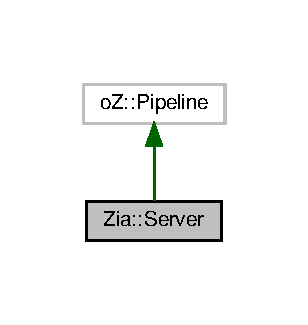
\includegraphics[width=148pt]{class_zia_1_1_server__inherit__graph}
\end{center}
\end{figure}


Collaboration diagram for Zia\+:\+:Server\+:\nopagebreak
\begin{figure}[H]
\begin{center}
\leavevmode
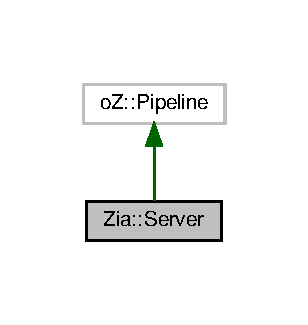
\includegraphics[width=148pt]{class_zia_1_1_server__coll__graph}
\end{center}
\end{figure}
\subsection*{Public Types}
\begin{DoxyCompactItemize}
\item 
using \hyperlink{class_zia_1_1_server_a10861064c5ac1dc97cc537023d67471d}{Config\+Ptr} = std\+::shared\+\_\+ptr$<$ \hyperlink{class_zia_1_1_server_config}{Server\+Config} $>$
\item 
using \hyperlink{class_zia_1_1_server_a624c715504f8bbf6b858081dabe26f9c}{io\+\_\+service} = boost\+::asio\+::io\+\_\+service
\item 
using \hyperlink{class_zia_1_1_server_a0119259e0eaa12e4f688c6c64dbf6ac0}{Acceptor} = boost\+::asio\+::ip\+::tcp\+::acceptor
\item 
using \hyperlink{class_zia_1_1_server_ae3a52a854f930c1daa7c8e510f7e37bd}{Socket} = boost\+::asio\+::ip\+::tcp\+::socket
\item 
using \hyperlink{class_zia_1_1_server_a4764ec255c11f5b7fb87f5ab1d44e952}{Endpoint} = boost\+::asio\+::ip\+::tcp\+::endpoint
\end{DoxyCompactItemize}
\subsection*{Public Member Functions}
\begin{DoxyCompactItemize}
\item 
\hyperlink{class_zia_1_1_server_a3f1591f28c6755b353d61e3a44d56b39}{Server} (const \hyperlink{class_zia_1_1_server_a10861064c5ac1dc97cc537023d67471d}{Config\+Ptr} \&config)
\item 
void \hyperlink{class_zia_1_1_server_abb27d30b40a94326e3fd629d3b30b7d5}{run} ()
\begin{DoxyCompactList}\small\item\em Run \hyperlink{class_zia_1_1_server}{Server}. \end{DoxyCompactList}\item 
void \hyperlink{class_zia_1_1_server_ad1a4b1650214d156491a98ff6b96d787}{close} ()
\begin{DoxyCompactList}\small\item\em Close \hyperlink{class_zia_1_1_server}{Server}. \end{DoxyCompactList}\end{DoxyCompactItemize}


\subsection{Detailed Description}
\hyperlink{class_zia_1_1_server}{Server} class to manage the server. 

Definition at line 22 of file Server.\+hpp.



\subsection{Member Typedef Documentation}
\mbox{\Hypertarget{class_zia_1_1_server_a0119259e0eaa12e4f688c6c64dbf6ac0}\label{class_zia_1_1_server_a0119259e0eaa12e4f688c6c64dbf6ac0}} 
\index{Zia\+::\+Server@{Zia\+::\+Server}!Acceptor@{Acceptor}}
\index{Acceptor@{Acceptor}!Zia\+::\+Server@{Zia\+::\+Server}}
\subsubsection{\texorpdfstring{Acceptor}{Acceptor}}
{\footnotesize\ttfamily using \hyperlink{class_zia_1_1_server_a0119259e0eaa12e4f688c6c64dbf6ac0}{Zia\+::\+Server\+::\+Acceptor} =  boost\+::asio\+::ip\+::tcp\+::acceptor}



Definition at line 29 of file Server.\+hpp.

\mbox{\Hypertarget{class_zia_1_1_server_a10861064c5ac1dc97cc537023d67471d}\label{class_zia_1_1_server_a10861064c5ac1dc97cc537023d67471d}} 
\index{Zia\+::\+Server@{Zia\+::\+Server}!Config\+Ptr@{Config\+Ptr}}
\index{Config\+Ptr@{Config\+Ptr}!Zia\+::\+Server@{Zia\+::\+Server}}
\subsubsection{\texorpdfstring{Config\+Ptr}{ConfigPtr}}
{\footnotesize\ttfamily using \hyperlink{class_zia_1_1_server_a10861064c5ac1dc97cc537023d67471d}{Zia\+::\+Server\+::\+Config\+Ptr} =  std\+::shared\+\_\+ptr$<$\hyperlink{class_zia_1_1_server_config}{Server\+Config}$>$}



Definition at line 25 of file Server.\+hpp.

\mbox{\Hypertarget{class_zia_1_1_server_a4764ec255c11f5b7fb87f5ab1d44e952}\label{class_zia_1_1_server_a4764ec255c11f5b7fb87f5ab1d44e952}} 
\index{Zia\+::\+Server@{Zia\+::\+Server}!Endpoint@{Endpoint}}
\index{Endpoint@{Endpoint}!Zia\+::\+Server@{Zia\+::\+Server}}
\subsubsection{\texorpdfstring{Endpoint}{Endpoint}}
{\footnotesize\ttfamily using \hyperlink{class_zia_1_1_server_a4764ec255c11f5b7fb87f5ab1d44e952}{Zia\+::\+Server\+::\+Endpoint} =  boost\+::asio\+::ip\+::tcp\+::endpoint}



Definition at line 33 of file Server.\+hpp.

\mbox{\Hypertarget{class_zia_1_1_server_a624c715504f8bbf6b858081dabe26f9c}\label{class_zia_1_1_server_a624c715504f8bbf6b858081dabe26f9c}} 
\index{Zia\+::\+Server@{Zia\+::\+Server}!io\+\_\+service@{io\+\_\+service}}
\index{io\+\_\+service@{io\+\_\+service}!Zia\+::\+Server@{Zia\+::\+Server}}
\subsubsection{\texorpdfstring{io\+\_\+service}{io\_service}}
{\footnotesize\ttfamily using \hyperlink{class_zia_1_1_server_a624c715504f8bbf6b858081dabe26f9c}{Zia\+::\+Server\+::io\+\_\+service} =  boost\+::asio\+::io\+\_\+service}



Definition at line 27 of file Server.\+hpp.

\mbox{\Hypertarget{class_zia_1_1_server_ae3a52a854f930c1daa7c8e510f7e37bd}\label{class_zia_1_1_server_ae3a52a854f930c1daa7c8e510f7e37bd}} 
\index{Zia\+::\+Server@{Zia\+::\+Server}!Socket@{Socket}}
\index{Socket@{Socket}!Zia\+::\+Server@{Zia\+::\+Server}}
\subsubsection{\texorpdfstring{Socket}{Socket}}
{\footnotesize\ttfamily using \hyperlink{class_zia_1_1_server_ae3a52a854f930c1daa7c8e510f7e37bd}{Zia\+::\+Server\+::\+Socket} =  boost\+::asio\+::ip\+::tcp\+::socket}



Definition at line 31 of file Server.\+hpp.



\subsection{Constructor \& Destructor Documentation}
\mbox{\Hypertarget{class_zia_1_1_server_a3f1591f28c6755b353d61e3a44d56b39}\label{class_zia_1_1_server_a3f1591f28c6755b353d61e3a44d56b39}} 
\index{Zia\+::\+Server@{Zia\+::\+Server}!Server@{Server}}
\index{Server@{Server}!Zia\+::\+Server@{Zia\+::\+Server}}
\subsubsection{\texorpdfstring{Server()}{Server()}}
{\footnotesize\ttfamily Server\+::\+Server (\begin{DoxyParamCaption}\item[{const \hyperlink{class_zia_1_1_server_a10861064c5ac1dc97cc537023d67471d}{Config\+Ptr} \&}]{config }\end{DoxyParamCaption})}



Definition at line 17 of file Server.\+cpp.



\subsection{Member Function Documentation}
\mbox{\Hypertarget{class_zia_1_1_server_ad1a4b1650214d156491a98ff6b96d787}\label{class_zia_1_1_server_ad1a4b1650214d156491a98ff6b96d787}} 
\index{Zia\+::\+Server@{Zia\+::\+Server}!close@{close}}
\index{close@{close}!Zia\+::\+Server@{Zia\+::\+Server}}
\subsubsection{\texorpdfstring{close()}{close()}}
{\footnotesize\ttfamily void Server\+::close (\begin{DoxyParamCaption}{ }\end{DoxyParamCaption})}



Close \hyperlink{class_zia_1_1_server}{Server}. 



Definition at line 61 of file Server.\+cpp.

\mbox{\Hypertarget{class_zia_1_1_server_abb27d30b40a94326e3fd629d3b30b7d5}\label{class_zia_1_1_server_abb27d30b40a94326e3fd629d3b30b7d5}} 
\index{Zia\+::\+Server@{Zia\+::\+Server}!run@{run}}
\index{run@{run}!Zia\+::\+Server@{Zia\+::\+Server}}
\subsubsection{\texorpdfstring{run()}{run()}}
{\footnotesize\ttfamily void Server\+::run (\begin{DoxyParamCaption}{ }\end{DoxyParamCaption})}



Run \hyperlink{class_zia_1_1_server}{Server}. 



Definition at line 56 of file Server.\+cpp.



The documentation for this class was generated from the following files\+:\begin{DoxyCompactItemize}
\item 
src/server/\hyperlink{_server_8hpp}{Server.\+hpp}\item 
src/server/\hyperlink{_server_8cpp}{Server.\+cpp}\end{DoxyCompactItemize}

\hypertarget{class_zia_1_1_server_config}{}\section{Zia\+:\+:Server\+Config Class Reference}
\label{class_zia_1_1_server_config}\index{Zia\+::\+Server\+Config@{Zia\+::\+Server\+Config}}


\hyperlink{class_zia_1_1_server_config}{Server\+Config} class to manage configuration files of the server.  




{\ttfamily \#include $<$Server\+Config.\+hpp$>$}



Inheritance diagram for Zia\+:\+:Server\+Config\+:\nopagebreak
\begin{figure}[H]
\begin{center}
\leavevmode
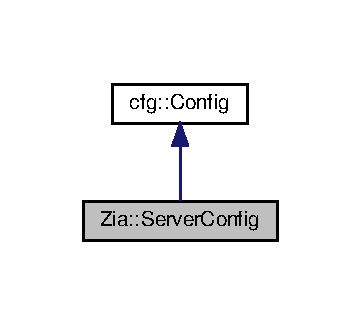
\includegraphics[width=173pt]{class_zia_1_1_server_config__inherit__graph}
\end{center}
\end{figure}


Collaboration diagram for Zia\+:\+:Server\+Config\+:\nopagebreak
\begin{figure}[H]
\begin{center}
\leavevmode
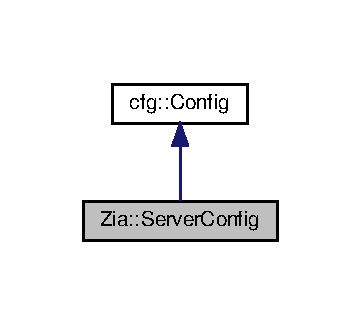
\includegraphics[width=173pt]{class_zia_1_1_server_config__coll__graph}
\end{center}
\end{figure}
\subsection*{Public Member Functions}
\begin{DoxyCompactItemize}
\item 
\hyperlink{class_zia_1_1_server_config_a1a98af732891f93c29f588b5377d4cb2}{Server\+Config} (const \hyperlink{namespacecfg_af0aed6e47bd26e91ad7d69467f96caaf}{File\+Descriptor} \&file, const std\+::string \&name)
\begin{DoxyCompactList}\small\item\em Construct a new \hyperlink{class_zia_1_1_server_config}{Server\+Config} object. \end{DoxyCompactList}\item 
\hyperlink{class_zia_1_1_server_config_aed6f704e1b0c3fa4b7abe44d7dcc3d06}{$\sim$\+Server\+Config} ()=default
\begin{DoxyCompactList}\small\item\em Destroy the \hyperlink{class_zia_1_1_server_config}{Server\+Config} object. \end{DoxyCompactList}\item 
void \hyperlink{class_zia_1_1_server_config_ad50ff700e0dd38f66017ce229f89717e}{load\+Config} (const std\+::filesystem\+::path \&path)
\begin{DoxyCompactList}\small\item\em Load configuration from a given file. \end{DoxyCompactList}\item 
void \hyperlink{class_zia_1_1_server_config_a4467dc6237876b82ad5970b2f6ee1966}{update\+Enabled\+Modules\+List} ()
\begin{DoxyCompactList}\small\item\em Update list of enabled modules. \end{DoxyCompactList}\item 
const std\+::string \hyperlink{class_zia_1_1_server_config_a0df081f26973e1a5182adf8f3d6495ae}{get\+Address} () const noexcept
\item 
const int \hyperlink{class_zia_1_1_server_config_ad8095c8981f48e9fa4112de41d4e6657}{get\+Port} () const noexcept
\item 
std\+::string \hyperlink{class_zia_1_1_server_config_aaa1d6beade9709ef602149c669641da9}{get\+Config\+Path} () const noexcept
\item 
std\+::string \hyperlink{class_zia_1_1_server_config_ae55e57b14d9efafcbecc23bf5b8d3957}{get\+Modules\+Path} () const noexcept
\item 
const \hyperlink{namespace_zia_a3076ef33a6c08b068cb8e444848ad33c}{Enabled\+List} \hyperlink{class_zia_1_1_server_config_a3ee30a0d396ff60fc7d06110005654f3}{get\+Enabled\+Modules\+List} () const noexcept
\begin{DoxyCompactList}\small\item\em Get list of enabled modules. \end{DoxyCompactList}\item 
const std\+::string \hyperlink{class_zia_1_1_server_config_a931a626c641223c2136979ef4c1aafe9}{get\+Module\+Name} (const std\+::string \&filename) const
\item 
const std\+::string \hyperlink{class_zia_1_1_server_config_a090ae222eeed278436a1fba19f5dcd6c}{get\+Module\+Name} (const \hyperlink{namespacecfg_af0aed6e47bd26e91ad7d69467f96caaf}{File\+Descriptor} \&file) const
\end{DoxyCompactItemize}


\subsection{Detailed Description}
\hyperlink{class_zia_1_1_server_config}{Server\+Config} class to manage configuration files of the server. 

Definition at line 52 of file Server\+Config.\+hpp.



\subsection{Constructor \& Destructor Documentation}
\mbox{\Hypertarget{class_zia_1_1_server_config_a1a98af732891f93c29f588b5377d4cb2}\label{class_zia_1_1_server_config_a1a98af732891f93c29f588b5377d4cb2}} 
\index{Zia\+::\+Server\+Config@{Zia\+::\+Server\+Config}!Server\+Config@{Server\+Config}}
\index{Server\+Config@{Server\+Config}!Zia\+::\+Server\+Config@{Zia\+::\+Server\+Config}}
\subsubsection{\texorpdfstring{Server\+Config()}{ServerConfig()}}
{\footnotesize\ttfamily Server\+Config\+::\+Server\+Config (\begin{DoxyParamCaption}\item[{const \hyperlink{namespacecfg_af0aed6e47bd26e91ad7d69467f96caaf}{File\+Descriptor} \&}]{file,  }\item[{const std\+::string \&}]{name }\end{DoxyParamCaption})}



Construct a new \hyperlink{class_zia_1_1_server_config}{Server\+Config} object. 


\begin{DoxyParams}{Parameters}
{\em file} & File descriptor of the associated json configuration file. \\
\hline
{\em name} & Registration name of the \hyperlink{class_zia_1_1_server_config}{Server\+Config} object. \\
\hline
\end{DoxyParams}


Definition at line 12 of file Server\+Config.\+cpp.

\mbox{\Hypertarget{class_zia_1_1_server_config_aed6f704e1b0c3fa4b7abe44d7dcc3d06}\label{class_zia_1_1_server_config_aed6f704e1b0c3fa4b7abe44d7dcc3d06}} 
\index{Zia\+::\+Server\+Config@{Zia\+::\+Server\+Config}!````~Server\+Config@{$\sim$\+Server\+Config}}
\index{````~Server\+Config@{$\sim$\+Server\+Config}!Zia\+::\+Server\+Config@{Zia\+::\+Server\+Config}}
\subsubsection{\texorpdfstring{$\sim$\+Server\+Config()}{~ServerConfig()}}
{\footnotesize\ttfamily Zia\+::\+Server\+Config\+::$\sim$\+Server\+Config (\begin{DoxyParamCaption}{ }\end{DoxyParamCaption})\hspace{0.3cm}{\ttfamily [default]}}



Destroy the \hyperlink{class_zia_1_1_server_config}{Server\+Config} object. 



\subsection{Member Function Documentation}
\mbox{\Hypertarget{class_zia_1_1_server_config_a0df081f26973e1a5182adf8f3d6495ae}\label{class_zia_1_1_server_config_a0df081f26973e1a5182adf8f3d6495ae}} 
\index{Zia\+::\+Server\+Config@{Zia\+::\+Server\+Config}!get\+Address@{get\+Address}}
\index{get\+Address@{get\+Address}!Zia\+::\+Server\+Config@{Zia\+::\+Server\+Config}}
\subsubsection{\texorpdfstring{get\+Address()}{getAddress()}}
{\footnotesize\ttfamily const std\+::string Server\+Config\+::get\+Address (\begin{DoxyParamCaption}{ }\end{DoxyParamCaption}) const\hspace{0.3cm}{\ttfamily [noexcept]}}



Definition at line 54 of file Server\+Config.\+cpp.

\mbox{\Hypertarget{class_zia_1_1_server_config_aaa1d6beade9709ef602149c669641da9}\label{class_zia_1_1_server_config_aaa1d6beade9709ef602149c669641da9}} 
\index{Zia\+::\+Server\+Config@{Zia\+::\+Server\+Config}!get\+Config\+Path@{get\+Config\+Path}}
\index{get\+Config\+Path@{get\+Config\+Path}!Zia\+::\+Server\+Config@{Zia\+::\+Server\+Config}}
\subsubsection{\texorpdfstring{get\+Config\+Path()}{getConfigPath()}}
{\footnotesize\ttfamily std\+::string Server\+Config\+::get\+Config\+Path (\begin{DoxyParamCaption}{ }\end{DoxyParamCaption}) const\hspace{0.3cm}{\ttfamily [noexcept]}}



Definition at line 64 of file Server\+Config.\+cpp.

\mbox{\Hypertarget{class_zia_1_1_server_config_a3ee30a0d396ff60fc7d06110005654f3}\label{class_zia_1_1_server_config_a3ee30a0d396ff60fc7d06110005654f3}} 
\index{Zia\+::\+Server\+Config@{Zia\+::\+Server\+Config}!get\+Enabled\+Modules\+List@{get\+Enabled\+Modules\+List}}
\index{get\+Enabled\+Modules\+List@{get\+Enabled\+Modules\+List}!Zia\+::\+Server\+Config@{Zia\+::\+Server\+Config}}
\subsubsection{\texorpdfstring{get\+Enabled\+Modules\+List()}{getEnabledModulesList()}}
{\footnotesize\ttfamily const \hyperlink{namespace_zia_a3076ef33a6c08b068cb8e444848ad33c}{Enabled\+List} Server\+Config\+::get\+Enabled\+Modules\+List (\begin{DoxyParamCaption}{ }\end{DoxyParamCaption}) const\hspace{0.3cm}{\ttfamily [noexcept]}}



Get list of enabled modules. 

\begin{DoxyReturn}{Returns}
List of enabled modules as Enabled\+List type. 
\end{DoxyReturn}


Definition at line 74 of file Server\+Config.\+cpp.

\mbox{\Hypertarget{class_zia_1_1_server_config_a931a626c641223c2136979ef4c1aafe9}\label{class_zia_1_1_server_config_a931a626c641223c2136979ef4c1aafe9}} 
\index{Zia\+::\+Server\+Config@{Zia\+::\+Server\+Config}!get\+Module\+Name@{get\+Module\+Name}}
\index{get\+Module\+Name@{get\+Module\+Name}!Zia\+::\+Server\+Config@{Zia\+::\+Server\+Config}}
\subsubsection{\texorpdfstring{get\+Module\+Name()}{getModuleName()}\hspace{0.1cm}{\footnotesize\ttfamily [1/2]}}
{\footnotesize\ttfamily const std\+::string Server\+Config\+::get\+Module\+Name (\begin{DoxyParamCaption}\item[{const std\+::string \&}]{filename }\end{DoxyParamCaption}) const}



Definition at line 79 of file Server\+Config.\+cpp.

\mbox{\Hypertarget{class_zia_1_1_server_config_a090ae222eeed278436a1fba19f5dcd6c}\label{class_zia_1_1_server_config_a090ae222eeed278436a1fba19f5dcd6c}} 
\index{Zia\+::\+Server\+Config@{Zia\+::\+Server\+Config}!get\+Module\+Name@{get\+Module\+Name}}
\index{get\+Module\+Name@{get\+Module\+Name}!Zia\+::\+Server\+Config@{Zia\+::\+Server\+Config}}
\subsubsection{\texorpdfstring{get\+Module\+Name()}{getModuleName()}\hspace{0.1cm}{\footnotesize\ttfamily [2/2]}}
{\footnotesize\ttfamily const std\+::string Server\+Config\+::get\+Module\+Name (\begin{DoxyParamCaption}\item[{const \hyperlink{namespacecfg_af0aed6e47bd26e91ad7d69467f96caaf}{File\+Descriptor} \&}]{file }\end{DoxyParamCaption}) const}



Definition at line 86 of file Server\+Config.\+cpp.

\mbox{\Hypertarget{class_zia_1_1_server_config_ae55e57b14d9efafcbecc23bf5b8d3957}\label{class_zia_1_1_server_config_ae55e57b14d9efafcbecc23bf5b8d3957}} 
\index{Zia\+::\+Server\+Config@{Zia\+::\+Server\+Config}!get\+Modules\+Path@{get\+Modules\+Path}}
\index{get\+Modules\+Path@{get\+Modules\+Path}!Zia\+::\+Server\+Config@{Zia\+::\+Server\+Config}}
\subsubsection{\texorpdfstring{get\+Modules\+Path()}{getModulesPath()}}
{\footnotesize\ttfamily std\+::string Server\+Config\+::get\+Modules\+Path (\begin{DoxyParamCaption}{ }\end{DoxyParamCaption}) const\hspace{0.3cm}{\ttfamily [noexcept]}}



Definition at line 69 of file Server\+Config.\+cpp.

\mbox{\Hypertarget{class_zia_1_1_server_config_ad8095c8981f48e9fa4112de41d4e6657}\label{class_zia_1_1_server_config_ad8095c8981f48e9fa4112de41d4e6657}} 
\index{Zia\+::\+Server\+Config@{Zia\+::\+Server\+Config}!get\+Port@{get\+Port}}
\index{get\+Port@{get\+Port}!Zia\+::\+Server\+Config@{Zia\+::\+Server\+Config}}
\subsubsection{\texorpdfstring{get\+Port()}{getPort()}}
{\footnotesize\ttfamily const int Server\+Config\+::get\+Port (\begin{DoxyParamCaption}{ }\end{DoxyParamCaption}) const\hspace{0.3cm}{\ttfamily [noexcept]}}



Definition at line 59 of file Server\+Config.\+cpp.

\mbox{\Hypertarget{class_zia_1_1_server_config_ad50ff700e0dd38f66017ce229f89717e}\label{class_zia_1_1_server_config_ad50ff700e0dd38f66017ce229f89717e}} 
\index{Zia\+::\+Server\+Config@{Zia\+::\+Server\+Config}!load\+Config@{load\+Config}}
\index{load\+Config@{load\+Config}!Zia\+::\+Server\+Config@{Zia\+::\+Server\+Config}}
\subsubsection{\texorpdfstring{load\+Config()}{loadConfig()}}
{\footnotesize\ttfamily void Server\+Config\+::load\+Config (\begin{DoxyParamCaption}\item[{const std\+::filesystem\+::path \&}]{path }\end{DoxyParamCaption})}



Load configuration from a given file. 


\begin{DoxyParams}{Parameters}
{\em path} & Path to the configuration file. \\
\hline
\end{DoxyParams}


Definition at line 20 of file Server\+Config.\+cpp.

\mbox{\Hypertarget{class_zia_1_1_server_config_a4467dc6237876b82ad5970b2f6ee1966}\label{class_zia_1_1_server_config_a4467dc6237876b82ad5970b2f6ee1966}} 
\index{Zia\+::\+Server\+Config@{Zia\+::\+Server\+Config}!update\+Enabled\+Modules\+List@{update\+Enabled\+Modules\+List}}
\index{update\+Enabled\+Modules\+List@{update\+Enabled\+Modules\+List}!Zia\+::\+Server\+Config@{Zia\+::\+Server\+Config}}
\subsubsection{\texorpdfstring{update\+Enabled\+Modules\+List()}{updateEnabledModulesList()}}
{\footnotesize\ttfamily void Server\+Config\+::update\+Enabled\+Modules\+List (\begin{DoxyParamCaption}{ }\end{DoxyParamCaption})}



Update list of enabled modules. 



Definition at line 36 of file Server\+Config.\+cpp.



The documentation for this class was generated from the following files\+:\begin{DoxyCompactItemize}
\item 
src/server/\hyperlink{_server_config_8hpp}{Server\+Config.\+hpp}\item 
src/server/\hyperlink{_server_config_8cpp}{Server\+Config.\+cpp}\end{DoxyCompactItemize}

\hypertarget{class_shared_memory}{}\section{Shared\+Memory Class Reference}
\label{class_shared_memory}\index{Shared\+Memory@{Shared\+Memory}}


{\ttfamily \#include $<$Shared\+Memory.\+hpp$>$}

\subsection*{Public Member Functions}
\begin{DoxyCompactItemize}
\item 
\hyperlink{class_shared_memory_a851a8d425f9c1e6f49237efd97628df5}{Shared\+Memory} ()=default
\item 
\hyperlink{class_shared_memory_a7467ee9b4149f66e660b0af3f0706a51}{$\sim$\+Shared\+Memory} ()=default
\item 
void \hyperlink{class_shared_memory_a49a12f61b3b8bd4811a1351c434dd121}{write\+\_\+data} (key\+\_\+t, size\+\_\+t, size\+\_\+t, std\+::string)
\item 
char $\ast$ \hyperlink{class_shared_memory_a35b6a9038b69b6abd3128cd028670cf6}{get\+\_\+data} (key\+\_\+t, size\+\_\+t, size\+\_\+t) const
\item 
char $\ast$ \hyperlink{class_shared_memory_a209fcce32c646bd4ad4e2492004b32c5}{get\+\_\+data\+\_\+by\+\_\+id} (int) const
\item 
void \hyperlink{class_shared_memory_af5531b0b30d05f359719e406886aa61e}{detach\+\_\+from} (const void $\ast$)
\end{DoxyCompactItemize}
\subsection*{Static Public Member Functions}
\begin{DoxyCompactItemize}
\item 
static void \hyperlink{class_shared_memory_a747779f81bac44bdf42172160199cfe2}{destroy} (int, int)
\item 
static key\+\_\+t \hyperlink{class_shared_memory_a05547eb8707ee646607334893b4196c3}{key\+\_\+gen} (std\+::string, int)
\item 
static int \hyperlink{class_shared_memory_af171de2b17ae37c2e19a0980000d2f60}{id\+\_\+gen} (key\+\_\+t, size\+\_\+t, size\+\_\+t)
\end{DoxyCompactItemize}


\subsection{Detailed Description}


Definition at line 18 of file Shared\+Memory.\+hpp.



\subsection{Constructor \& Destructor Documentation}
\mbox{\Hypertarget{class_shared_memory_a851a8d425f9c1e6f49237efd97628df5}\label{class_shared_memory_a851a8d425f9c1e6f49237efd97628df5}} 
\index{Shared\+Memory@{Shared\+Memory}!Shared\+Memory@{Shared\+Memory}}
\index{Shared\+Memory@{Shared\+Memory}!Shared\+Memory@{Shared\+Memory}}
\subsubsection{\texorpdfstring{Shared\+Memory()}{SharedMemory()}}
{\footnotesize\ttfamily Shared\+Memory\+::\+Shared\+Memory (\begin{DoxyParamCaption}{ }\end{DoxyParamCaption})\hspace{0.3cm}{\ttfamily [default]}}

\mbox{\Hypertarget{class_shared_memory_a7467ee9b4149f66e660b0af3f0706a51}\label{class_shared_memory_a7467ee9b4149f66e660b0af3f0706a51}} 
\index{Shared\+Memory@{Shared\+Memory}!````~Shared\+Memory@{$\sim$\+Shared\+Memory}}
\index{````~Shared\+Memory@{$\sim$\+Shared\+Memory}!Shared\+Memory@{Shared\+Memory}}
\subsubsection{\texorpdfstring{$\sim$\+Shared\+Memory()}{~SharedMemory()}}
{\footnotesize\ttfamily Shared\+Memory\+::$\sim$\+Shared\+Memory (\begin{DoxyParamCaption}{ }\end{DoxyParamCaption})\hspace{0.3cm}{\ttfamily [default]}}



\subsection{Member Function Documentation}
\mbox{\Hypertarget{class_shared_memory_a747779f81bac44bdf42172160199cfe2}\label{class_shared_memory_a747779f81bac44bdf42172160199cfe2}} 
\index{Shared\+Memory@{Shared\+Memory}!destroy@{destroy}}
\index{destroy@{destroy}!Shared\+Memory@{Shared\+Memory}}
\subsubsection{\texorpdfstring{destroy()}{destroy()}}
{\footnotesize\ttfamily void Shared\+Memory\+::destroy (\begin{DoxyParamCaption}\item[{int}]{shm\+Id,  }\item[{int}]{process }\end{DoxyParamCaption})\hspace{0.3cm}{\ttfamily [static]}}



Definition at line 43 of file Shared\+Memory.\+cpp.

\mbox{\Hypertarget{class_shared_memory_af5531b0b30d05f359719e406886aa61e}\label{class_shared_memory_af5531b0b30d05f359719e406886aa61e}} 
\index{Shared\+Memory@{Shared\+Memory}!detach\+\_\+from@{detach\+\_\+from}}
\index{detach\+\_\+from@{detach\+\_\+from}!Shared\+Memory@{Shared\+Memory}}
\subsubsection{\texorpdfstring{detach\+\_\+from()}{detach\_from()}}
{\footnotesize\ttfamily void Shared\+Memory\+::detach\+\_\+from (\begin{DoxyParamCaption}\item[{const void $\ast$}]{data }\end{DoxyParamCaption})}



Definition at line 37 of file Shared\+Memory.\+cpp.

\mbox{\Hypertarget{class_shared_memory_a35b6a9038b69b6abd3128cd028670cf6}\label{class_shared_memory_a35b6a9038b69b6abd3128cd028670cf6}} 
\index{Shared\+Memory@{Shared\+Memory}!get\+\_\+data@{get\+\_\+data}}
\index{get\+\_\+data@{get\+\_\+data}!Shared\+Memory@{Shared\+Memory}}
\subsubsection{\texorpdfstring{get\+\_\+data()}{get\_data()}}
{\footnotesize\ttfamily char $\ast$ Shared\+Memory\+::get\+\_\+data (\begin{DoxyParamCaption}\item[{key\+\_\+t}]{key,  }\item[{size\+\_\+t}]{data\+\_\+size,  }\item[{size\+\_\+t}]{process }\end{DoxyParamCaption}) const}



Definition at line 20 of file Shared\+Memory.\+cpp.

\mbox{\Hypertarget{class_shared_memory_a209fcce32c646bd4ad4e2492004b32c5}\label{class_shared_memory_a209fcce32c646bd4ad4e2492004b32c5}} 
\index{Shared\+Memory@{Shared\+Memory}!get\+\_\+data\+\_\+by\+\_\+id@{get\+\_\+data\+\_\+by\+\_\+id}}
\index{get\+\_\+data\+\_\+by\+\_\+id@{get\+\_\+data\+\_\+by\+\_\+id}!Shared\+Memory@{Shared\+Memory}}
\subsubsection{\texorpdfstring{get\+\_\+data\+\_\+by\+\_\+id()}{get\_data\_by\_id()}}
{\footnotesize\ttfamily char $\ast$ Shared\+Memory\+::get\+\_\+data\+\_\+by\+\_\+id (\begin{DoxyParamCaption}\item[{int}]{shm\+Id }\end{DoxyParamCaption}) const}



Definition at line 28 of file Shared\+Memory.\+cpp.

\mbox{\Hypertarget{class_shared_memory_af171de2b17ae37c2e19a0980000d2f60}\label{class_shared_memory_af171de2b17ae37c2e19a0980000d2f60}} 
\index{Shared\+Memory@{Shared\+Memory}!id\+\_\+gen@{id\+\_\+gen}}
\index{id\+\_\+gen@{id\+\_\+gen}!Shared\+Memory@{Shared\+Memory}}
\subsubsection{\texorpdfstring{id\+\_\+gen()}{id\_gen()}}
{\footnotesize\ttfamily int Shared\+Memory\+::id\+\_\+gen (\begin{DoxyParamCaption}\item[{key\+\_\+t}]{key,  }\item[{size\+\_\+t}]{data\+\_\+size,  }\item[{size\+\_\+t}]{process }\end{DoxyParamCaption})\hspace{0.3cm}{\ttfamily [static]}}



Definition at line 54 of file Shared\+Memory.\+cpp.

\mbox{\Hypertarget{class_shared_memory_a05547eb8707ee646607334893b4196c3}\label{class_shared_memory_a05547eb8707ee646607334893b4196c3}} 
\index{Shared\+Memory@{Shared\+Memory}!key\+\_\+gen@{key\+\_\+gen}}
\index{key\+\_\+gen@{key\+\_\+gen}!Shared\+Memory@{Shared\+Memory}}
\subsubsection{\texorpdfstring{key\+\_\+gen()}{key\_gen()}}
{\footnotesize\ttfamily key\+\_\+t Shared\+Memory\+::key\+\_\+gen (\begin{DoxyParamCaption}\item[{std\+::string}]{pathname,  }\item[{int}]{proj\+\_\+id }\end{DoxyParamCaption})\hspace{0.3cm}{\ttfamily [static]}}



Definition at line 49 of file Shared\+Memory.\+cpp.

\mbox{\Hypertarget{class_shared_memory_a49a12f61b3b8bd4811a1351c434dd121}\label{class_shared_memory_a49a12f61b3b8bd4811a1351c434dd121}} 
\index{Shared\+Memory@{Shared\+Memory}!write\+\_\+data@{write\+\_\+data}}
\index{write\+\_\+data@{write\+\_\+data}!Shared\+Memory@{Shared\+Memory}}
\subsubsection{\texorpdfstring{write\+\_\+data()}{write\_data()}}
{\footnotesize\ttfamily void Shared\+Memory\+::write\+\_\+data (\begin{DoxyParamCaption}\item[{key\+\_\+t}]{key,  }\item[{size\+\_\+t}]{data\+\_\+size,  }\item[{size\+\_\+t}]{process,  }\item[{std\+::string}]{data }\end{DoxyParamCaption})}



Definition at line 11 of file Shared\+Memory.\+cpp.



The documentation for this class was generated from the following files\+:\begin{DoxyCompactItemize}
\item 
src/utils/\hyperlink{_shared_memory_8hpp}{Shared\+Memory.\+hpp}\item 
src/utils/\hyperlink{_shared_memory_8cpp}{Shared\+Memory.\+cpp}\end{DoxyCompactItemize}

\hypertarget{class_s_s_l_module}{}\section{S\+S\+L\+Module Class Reference}
\label{class_s_s_l_module}\index{S\+S\+L\+Module@{S\+S\+L\+Module}}


\hyperlink{class_s_s_l_module}{S\+S\+L\+Module} class to manage the S\+SL module.  




{\ttfamily \#include $<$S\+S\+L\+Module.\+hpp$>$}



Inheritance diagram for S\+S\+L\+Module\+:\nopagebreak
\begin{figure}[H]
\begin{center}
\leavevmode
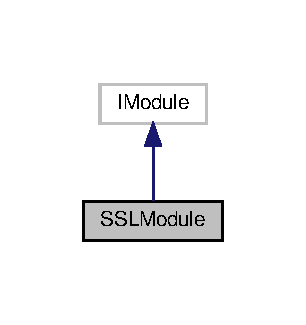
\includegraphics[width=147pt]{class_s_s_l_module__inherit__graph}
\end{center}
\end{figure}


Collaboration diagram for S\+S\+L\+Module\+:\nopagebreak
\begin{figure}[H]
\begin{center}
\leavevmode
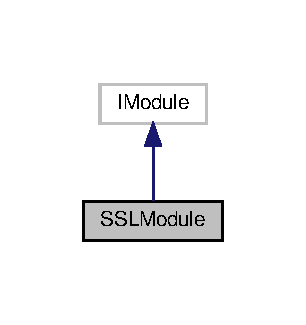
\includegraphics[width=147pt]{class_s_s_l_module__coll__graph}
\end{center}
\end{figure}
\subsection*{Public Member Functions}
\begin{DoxyCompactItemize}
\item 
\hyperlink{class_s_s_l_module_aff377c899776ca1e5ec94bb4b37e01db}{S\+S\+L\+Module} ()=default
\begin{DoxyCompactList}\small\item\em Default constructor for the ssl module. \end{DoxyCompactList}\item 
\hyperlink{class_s_s_l_module_a9d8061dd774544fb6eee57803b17f83d}{$\sim$\+S\+S\+L\+Module} ()
\begin{DoxyCompactList}\small\item\em Default destructor for the php module. \end{DoxyCompactList}\item 
virtual const char $\ast$ \hyperlink{class_s_s_l_module_a811d3b0f9f932791abbc89f1ecf2a1c3}{get\+Name} (void) const
\begin{DoxyCompactList}\small\item\em Get the name of the module. \end{DoxyCompactList}\item 
virtual void \hyperlink{class_s_s_l_module_ad2bcf5908355b434e45ea156a49f7d39}{on\+Register\+Callbacks} (o\+Z\+::\+Pipeline \&pipeline)
\begin{DoxyCompactList}\small\item\em Fct for the pipeline (load in the right place in the right position) \end{DoxyCompactList}\item 
virtual void \hyperlink{class_s_s_l_module_ac4592260a1fff11950ea1a20d2dd9729}{on\+Load\+Configuration\+File} (const std\+::string \&conf)
\begin{DoxyCompactList}\small\item\em Load the conf for the pipeline. \end{DoxyCompactList}\item 
virtual void \hyperlink{class_s_s_l_module_a514e3d618be55df6f5fc2f489e70d915}{on\+Connection} (const o\+Z\+::\+File\+Descriptor fd, const o\+Z\+::\+Endpoint endpoint, const bool use\+Encryption)
\begin{DoxyCompactList}\small\item\em Init the ssl lib. \end{DoxyCompactList}\item 
virtual void \hyperlink{class_s_s_l_module_a54cda727b3f282b0be43f132411edcd2}{on\+Disconnection} (const o\+Z\+::\+File\+Descriptor fd, const o\+Z\+::\+Endpoint endpoint)
\begin{DoxyCompactList}\small\item\em Destroy the ssl lib. \end{DoxyCompactList}\end{DoxyCompactItemize}


\subsection{Detailed Description}
\hyperlink{class_s_s_l_module}{S\+S\+L\+Module} class to manage the S\+SL module. 

Definition at line 26 of file S\+S\+L\+Module.\+hpp.



\subsection{Constructor \& Destructor Documentation}
\mbox{\Hypertarget{class_s_s_l_module_aff377c899776ca1e5ec94bb4b37e01db}\label{class_s_s_l_module_aff377c899776ca1e5ec94bb4b37e01db}} 
\index{S\+S\+L\+Module@{S\+S\+L\+Module}!S\+S\+L\+Module@{S\+S\+L\+Module}}
\index{S\+S\+L\+Module@{S\+S\+L\+Module}!S\+S\+L\+Module@{S\+S\+L\+Module}}
\subsubsection{\texorpdfstring{S\+S\+L\+Module()}{SSLModule()}}
{\footnotesize\ttfamily S\+S\+L\+Module\+::\+S\+S\+L\+Module (\begin{DoxyParamCaption}{ }\end{DoxyParamCaption})\hspace{0.3cm}{\ttfamily [default]}}



Default constructor for the ssl module. 

\mbox{\Hypertarget{class_s_s_l_module_a9d8061dd774544fb6eee57803b17f83d}\label{class_s_s_l_module_a9d8061dd774544fb6eee57803b17f83d}} 
\index{S\+S\+L\+Module@{S\+S\+L\+Module}!````~S\+S\+L\+Module@{$\sim$\+S\+S\+L\+Module}}
\index{````~S\+S\+L\+Module@{$\sim$\+S\+S\+L\+Module}!S\+S\+L\+Module@{S\+S\+L\+Module}}
\subsubsection{\texorpdfstring{$\sim$\+S\+S\+L\+Module()}{~SSLModule()}}
{\footnotesize\ttfamily S\+S\+L\+Module\+::$\sim$\+S\+S\+L\+Module (\begin{DoxyParamCaption}{ }\end{DoxyParamCaption})}



Default destructor for the php module. 



Definition at line 12 of file S\+S\+L\+Module.\+cpp.



\subsection{Member Function Documentation}
\mbox{\Hypertarget{class_s_s_l_module_a811d3b0f9f932791abbc89f1ecf2a1c3}\label{class_s_s_l_module_a811d3b0f9f932791abbc89f1ecf2a1c3}} 
\index{S\+S\+L\+Module@{S\+S\+L\+Module}!get\+Name@{get\+Name}}
\index{get\+Name@{get\+Name}!S\+S\+L\+Module@{S\+S\+L\+Module}}
\subsubsection{\texorpdfstring{get\+Name()}{getName()}}
{\footnotesize\ttfamily virtual const char$\ast$ S\+S\+L\+Module\+::get\+Name (\begin{DoxyParamCaption}\item[{void}]{ }\end{DoxyParamCaption}) const\hspace{0.3cm}{\ttfamily [inline]}, {\ttfamily [virtual]}}



Get the name of the module. 

\begin{DoxyReturn}{Returns}
The name of the module 
\end{DoxyReturn}


Definition at line 44 of file S\+S\+L\+Module.\+hpp.

\mbox{\Hypertarget{class_s_s_l_module_a514e3d618be55df6f5fc2f489e70d915}\label{class_s_s_l_module_a514e3d618be55df6f5fc2f489e70d915}} 
\index{S\+S\+L\+Module@{S\+S\+L\+Module}!on\+Connection@{on\+Connection}}
\index{on\+Connection@{on\+Connection}!S\+S\+L\+Module@{S\+S\+L\+Module}}
\subsubsection{\texorpdfstring{on\+Connection()}{onConnection()}}
{\footnotesize\ttfamily void S\+S\+L\+Module\+::on\+Connection (\begin{DoxyParamCaption}\item[{const o\+Z\+::\+File\+Descriptor}]{fd,  }\item[{const o\+Z\+::\+Endpoint}]{endpoint,  }\item[{const bool}]{use\+Encryption }\end{DoxyParamCaption})\hspace{0.3cm}{\ttfamily [virtual]}}



Init the ssl lib. 


\begin{DoxyParams}{Parameters}
{\em fd} & Fd open for the listen \\
\hline
{\em endpoint} & Endpoint use for the listen \\
\hline
{\em use\+Encryption} & Bool to know if it\textquotesingle{}s H\+T\+TP or H\+T\+T\+PS \\
\hline
\end{DoxyParams}


Definition at line 35 of file S\+S\+L\+Module.\+cpp.

\mbox{\Hypertarget{class_s_s_l_module_a54cda727b3f282b0be43f132411edcd2}\label{class_s_s_l_module_a54cda727b3f282b0be43f132411edcd2}} 
\index{S\+S\+L\+Module@{S\+S\+L\+Module}!on\+Disconnection@{on\+Disconnection}}
\index{on\+Disconnection@{on\+Disconnection}!S\+S\+L\+Module@{S\+S\+L\+Module}}
\subsubsection{\texorpdfstring{on\+Disconnection()}{onDisconnection()}}
{\footnotesize\ttfamily void S\+S\+L\+Module\+::on\+Disconnection (\begin{DoxyParamCaption}\item[{const o\+Z\+::\+File\+Descriptor}]{fd,  }\item[{const o\+Z\+::\+Endpoint}]{endpoint }\end{DoxyParamCaption})\hspace{0.3cm}{\ttfamily [virtual]}}



Destroy the ssl lib. 


\begin{DoxyParams}{Parameters}
{\em fd} & Fd close after the listen \\
\hline
{\em endpoint} & Endpoint close after the listen \\
\hline
\end{DoxyParams}


Definition at line 52 of file S\+S\+L\+Module.\+cpp.

\mbox{\Hypertarget{class_s_s_l_module_ac4592260a1fff11950ea1a20d2dd9729}\label{class_s_s_l_module_ac4592260a1fff11950ea1a20d2dd9729}} 
\index{S\+S\+L\+Module@{S\+S\+L\+Module}!on\+Load\+Configuration\+File@{on\+Load\+Configuration\+File}}
\index{on\+Load\+Configuration\+File@{on\+Load\+Configuration\+File}!S\+S\+L\+Module@{S\+S\+L\+Module}}
\subsubsection{\texorpdfstring{on\+Load\+Configuration\+File()}{onLoadConfigurationFile()}}
{\footnotesize\ttfamily void S\+S\+L\+Module\+::on\+Load\+Configuration\+File (\begin{DoxyParamCaption}\item[{const std\+::string \&}]{conf }\end{DoxyParamCaption})\hspace{0.3cm}{\ttfamily [virtual]}}



Load the conf for the pipeline. 


\begin{DoxyParams}{Parameters}
{\em conf} & Conf for modif the pipeline \\
\hline
\end{DoxyParams}


Definition at line 58 of file S\+S\+L\+Module.\+cpp.

\mbox{\Hypertarget{class_s_s_l_module_ad2bcf5908355b434e45ea156a49f7d39}\label{class_s_s_l_module_ad2bcf5908355b434e45ea156a49f7d39}} 
\index{S\+S\+L\+Module@{S\+S\+L\+Module}!on\+Register\+Callbacks@{on\+Register\+Callbacks}}
\index{on\+Register\+Callbacks@{on\+Register\+Callbacks}!S\+S\+L\+Module@{S\+S\+L\+Module}}
\subsubsection{\texorpdfstring{on\+Register\+Callbacks()}{onRegisterCallbacks()}}
{\footnotesize\ttfamily void S\+S\+L\+Module\+::on\+Register\+Callbacks (\begin{DoxyParamCaption}\item[{o\+Z\+::\+Pipeline \&}]{pipeline }\end{DoxyParamCaption})\hspace{0.3cm}{\ttfamily [virtual]}}



Fct for the pipeline (load in the right place in the right position) 


\begin{DoxyParams}{Parameters}
{\em pipeline} & Reference on the pipeline where the module is load \\
\hline
\end{DoxyParams}


Definition at line 20 of file S\+S\+L\+Module.\+cpp.



The documentation for this class was generated from the following files\+:\begin{DoxyCompactItemize}
\item 
src/modules/\+S\+S\+L/\hyperlink{_s_s_l_module_8hpp}{S\+S\+L\+Module.\+hpp}\item 
src/modules/\+S\+S\+L/\hyperlink{_s_s_l_module_8cpp}{S\+S\+L\+Module.\+cpp}\end{DoxyCompactItemize}

\chapter{File Documentation}
\hypertarget{_config_8cpp}{}\section{src/config/\+Config.cpp File Reference}
\label{_config_8cpp}\index{src/config/\+Config.\+cpp@{src/config/\+Config.\+cpp}}
{\ttfamily \#include \char`\"{}Config.\+hpp\char`\"{}}\newline
Include dependency graph for Config.\+cpp\+:\nopagebreak
\begin{figure}[H]
\begin{center}
\leavevmode
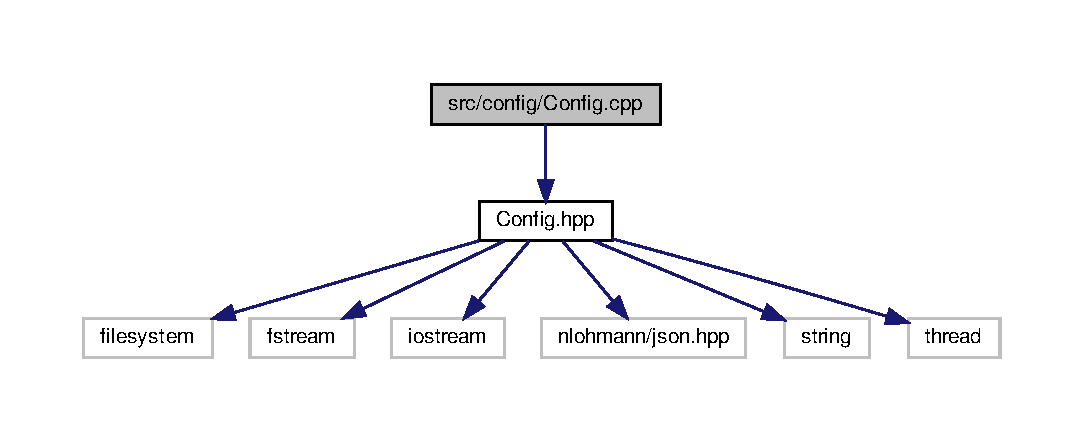
\includegraphics[width=350pt]{_config_8cpp__incl}
\end{center}
\end{figure}

\hypertarget{_config_8hpp}{}\section{src/config/\+Config.hpp File Reference}
\label{_config_8hpp}\index{src/config/\+Config.\+hpp@{src/config/\+Config.\+hpp}}
{\ttfamily \#include $<$filesystem$>$}\newline
{\ttfamily \#include $<$fstream$>$}\newline
{\ttfamily \#include $<$iostream$>$}\newline
{\ttfamily \#include $<$nlohmann/json.\+hpp$>$}\newline
{\ttfamily \#include $<$string$>$}\newline
{\ttfamily \#include $<$thread$>$}\newline
Include dependency graph for Config.\+hpp\+:\nopagebreak
\begin{figure}[H]
\begin{center}
\leavevmode
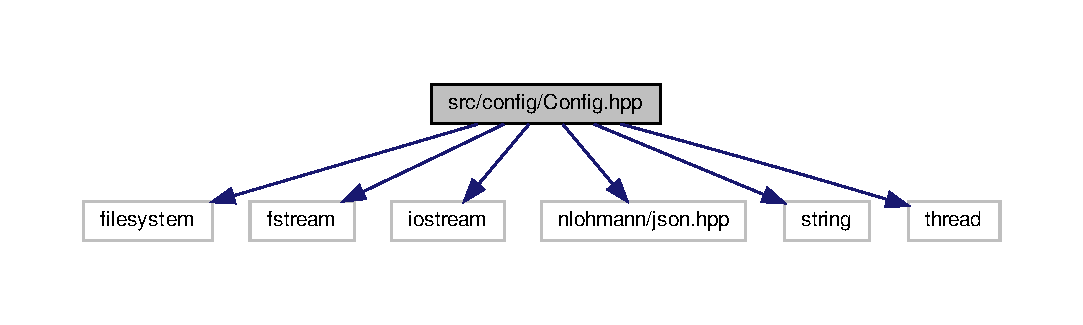
\includegraphics[width=350pt]{_config_8hpp__incl}
\end{center}
\end{figure}
This graph shows which files directly or indirectly include this file\+:\nopagebreak
\begin{figure}[H]
\begin{center}
\leavevmode
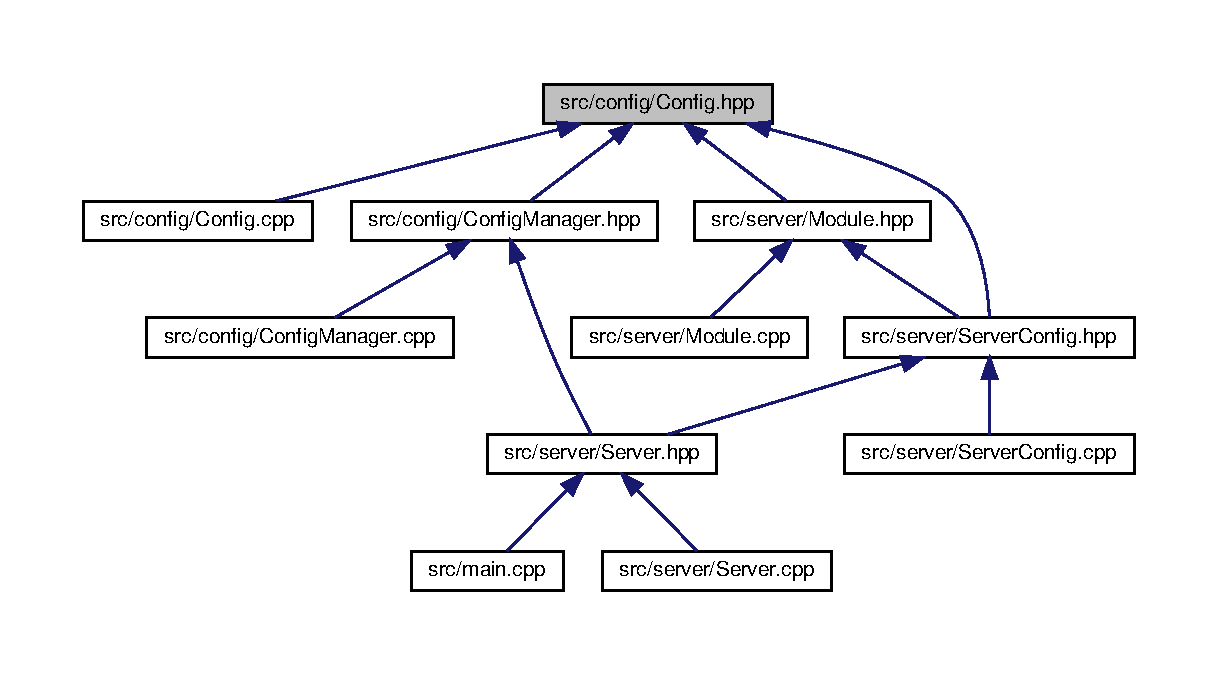
\includegraphics[width=350pt]{_config_8hpp__dep__incl}
\end{center}
\end{figure}
\subsection*{Classes}
\begin{DoxyCompactItemize}
\item 
class \hyperlink{classcfg_1_1_config}{cfg\+::\+Config}
\begin{DoxyCompactList}\small\item\em \hyperlink{classcfg_1_1_config}{Config} abstracts a configuration from a json file. \end{DoxyCompactList}\end{DoxyCompactItemize}
\subsection*{Namespaces}
\begin{DoxyCompactItemize}
\item 
 \hyperlink{namespacecfg}{cfg}
\end{DoxyCompactItemize}
\subsection*{Typedefs}
\begin{DoxyCompactItemize}
\item 
using \hyperlink{namespacecfg_af5f3a3fc2010c76e90bc66696485989f}{cfg\+::\+Config\+Ptr} = std\+::shared\+\_\+ptr$<$ Config $>$
\begin{DoxyCompactList}\small\item\em \hyperlink{classcfg_1_1_config}{Config} pointer type, using shared\+\_\+ptr as backend. \end{DoxyCompactList}\item 
using \hyperlink{namespacecfg_af0aed6e47bd26e91ad7d69467f96caaf}{cfg\+::\+File\+Descriptor} = std\+::filesystem\+::directory\+\_\+entry
\begin{DoxyCompactList}\small\item\em File descriptor from a directory entry. \end{DoxyCompactList}\item 
using \hyperlink{namespacecfg_aa17d58439174a5af7fb3f37a3cdd6d0b}{cfg\+::\+Timestamp} = std\+::filesystem\+::file\+\_\+time\+\_\+type
\begin{DoxyCompactList}\small\item\em File last modified date. \end{DoxyCompactList}\item 
using \hyperlink{namespacecfg_a4b03b67363586260311e07e8b27bd5ac}{cfg\+::json} = nlohmann\+::json
\begin{DoxyCompactList}\small\item\em Json library object. \end{DoxyCompactList}\end{DoxyCompactItemize}
\subsection*{Enumerations}
\begin{DoxyCompactItemize}
\item 
enum \hyperlink{namespacecfg_a384f743959a9029f7e1c3d11548795de}{cfg\+::\+File\+Status} \{ \hyperlink{namespacecfg_a384f743959a9029f7e1c3d11548795deae2fa538867c3830a859a5b17ab24644b}{cfg\+::\+File\+Status\+::created}, 
\hyperlink{namespacecfg_a384f743959a9029f7e1c3d11548795dea9ae73c65f418e6f79ceb4f0e4a4b98d5}{cfg\+::\+File\+Status\+::modified}, 
\hyperlink{namespacecfg_a384f743959a9029f7e1c3d11548795deaf4adee3fff79c6ddad5b2e45f730006a}{cfg\+::\+File\+Status\+::erased}, 
\hyperlink{namespacecfg_a384f743959a9029f7e1c3d11548795dea334c4a4c42fdb79d7ebc3e73b517e6f8}{cfg\+::\+File\+Status\+::none}
 \}\begin{DoxyCompactList}\small\item\em File status enumeration. \end{DoxyCompactList}
\end{DoxyCompactItemize}

\hypertarget{_config_manager_8cpp}{}\section{src/config/\+Config\+Manager.cpp File Reference}
\label{_config_manager_8cpp}\index{src/config/\+Config\+Manager.\+cpp@{src/config/\+Config\+Manager.\+cpp}}
{\ttfamily \#include \char`\"{}Config\+Manager.\+hpp\char`\"{}}\newline
Include dependency graph for Config\+Manager.\+cpp\+:\nopagebreak
\begin{figure}[H]
\begin{center}
\leavevmode
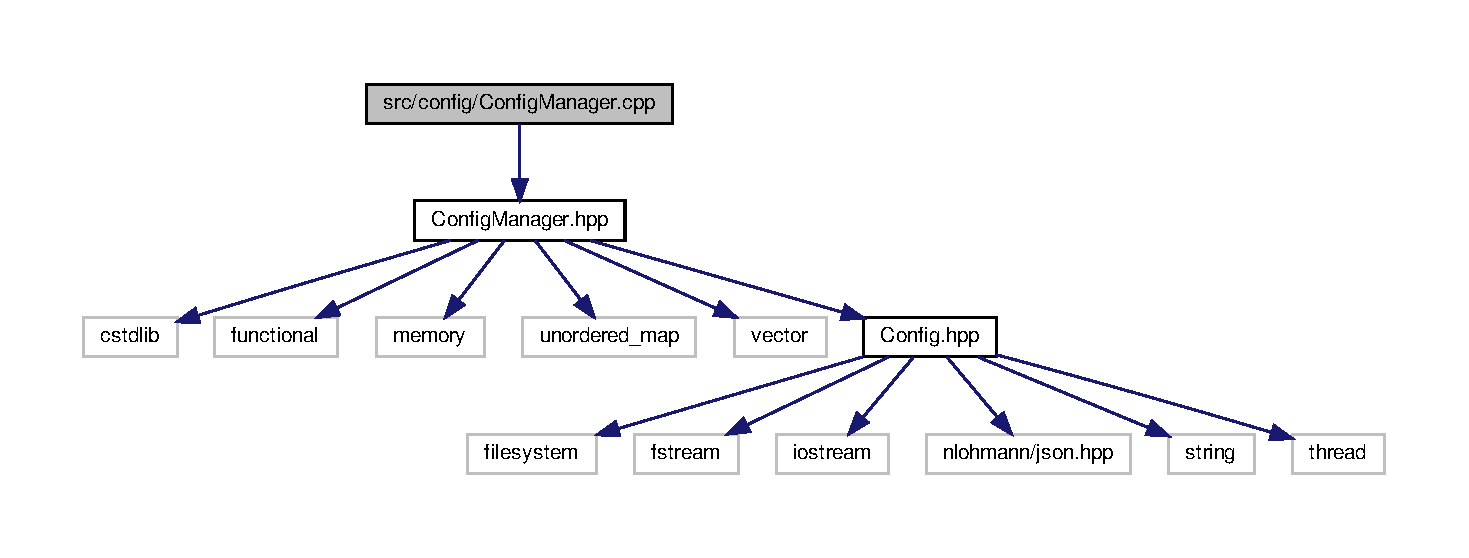
\includegraphics[width=350pt]{_config_manager_8cpp__incl}
\end{center}
\end{figure}

\hypertarget{_config_manager_8hpp}{}\section{src/config/\+Config\+Manager.hpp File Reference}
\label{_config_manager_8hpp}\index{src/config/\+Config\+Manager.\+hpp@{src/config/\+Config\+Manager.\+hpp}}
{\ttfamily \#include $<$cstdlib$>$}\newline
{\ttfamily \#include $<$functional$>$}\newline
{\ttfamily \#include $<$memory$>$}\newline
{\ttfamily \#include $<$unordered\+\_\+map$>$}\newline
{\ttfamily \#include $<$vector$>$}\newline
{\ttfamily \#include \char`\"{}Config.\+hpp\char`\"{}}\newline
Include dependency graph for Config\+Manager.\+hpp\+:\nopagebreak
\begin{figure}[H]
\begin{center}
\leavevmode
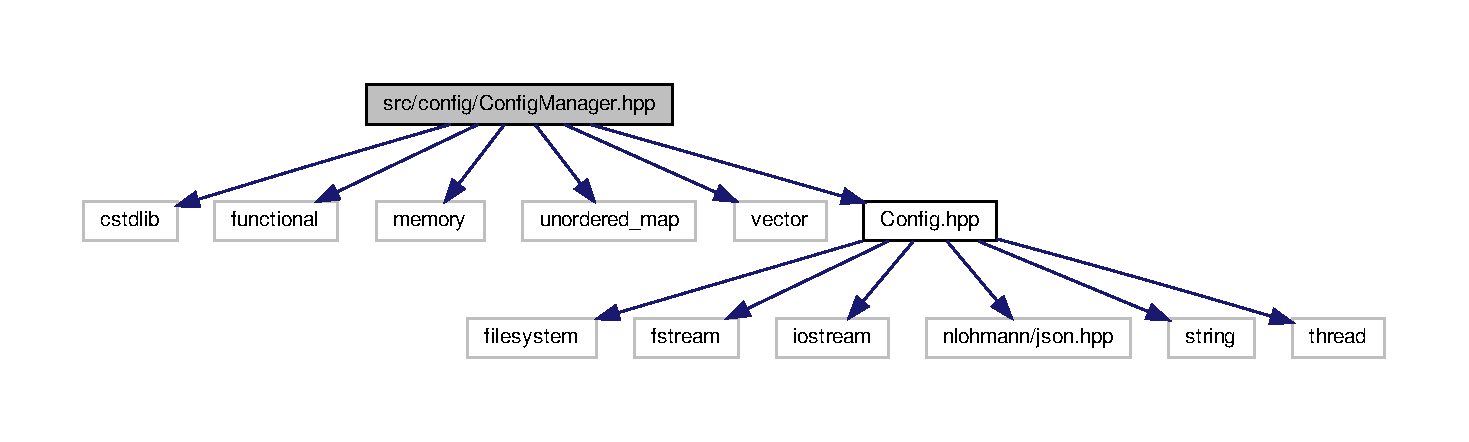
\includegraphics[width=350pt]{_config_manager_8hpp__incl}
\end{center}
\end{figure}
This graph shows which files directly or indirectly include this file\+:\nopagebreak
\begin{figure}[H]
\begin{center}
\leavevmode
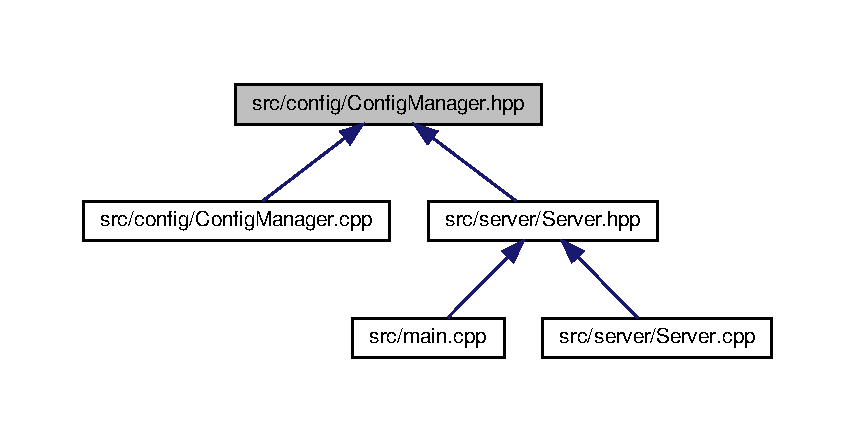
\includegraphics[width=350pt]{_config_manager_8hpp__dep__incl}
\end{center}
\end{figure}
\subsection*{Classes}
\begin{DoxyCompactItemize}
\item 
class \hyperlink{classcfg_1_1_config_manager}{cfg\+::\+Config\+Manager}
\begin{DoxyCompactList}\small\item\em \hyperlink{classcfg_1_1_config_manager}{Config\+Manager} class to manage the configuration files. \end{DoxyCompactList}\end{DoxyCompactItemize}
\subsection*{Namespaces}
\begin{DoxyCompactItemize}
\item 
 \hyperlink{namespacecfg}{cfg}
\end{DoxyCompactItemize}
\subsection*{Typedefs}
\begin{DoxyCompactItemize}
\item 
using \hyperlink{namespacecfg_ab1a8f7060b6dfea6111c4449e81c6f8c}{cfg\+::\+Time\+Sleep} = std\+::chrono\+::milliseconds
\begin{DoxyCompactList}\small\item\em Simple time unit of measuring. \end{DoxyCompactList}\end{DoxyCompactItemize}

\hypertarget{main_8cpp}{}\section{src/main.cpp File Reference}
\label{main_8cpp}\index{src/main.\+cpp@{src/main.\+cpp}}
{\ttfamily \#include $<$iostream$>$}\newline
{\ttfamily \#include $<$exception$>$}\newline
{\ttfamily \#include $<$server/\+Server.\+hpp$>$}\newline
{\ttfamily \#include $<$utils/\+Env\+Manager.\+hpp$>$}\newline
Include dependency graph for main.\+cpp\+:\nopagebreak
\begin{figure}[H]
\begin{center}
\leavevmode
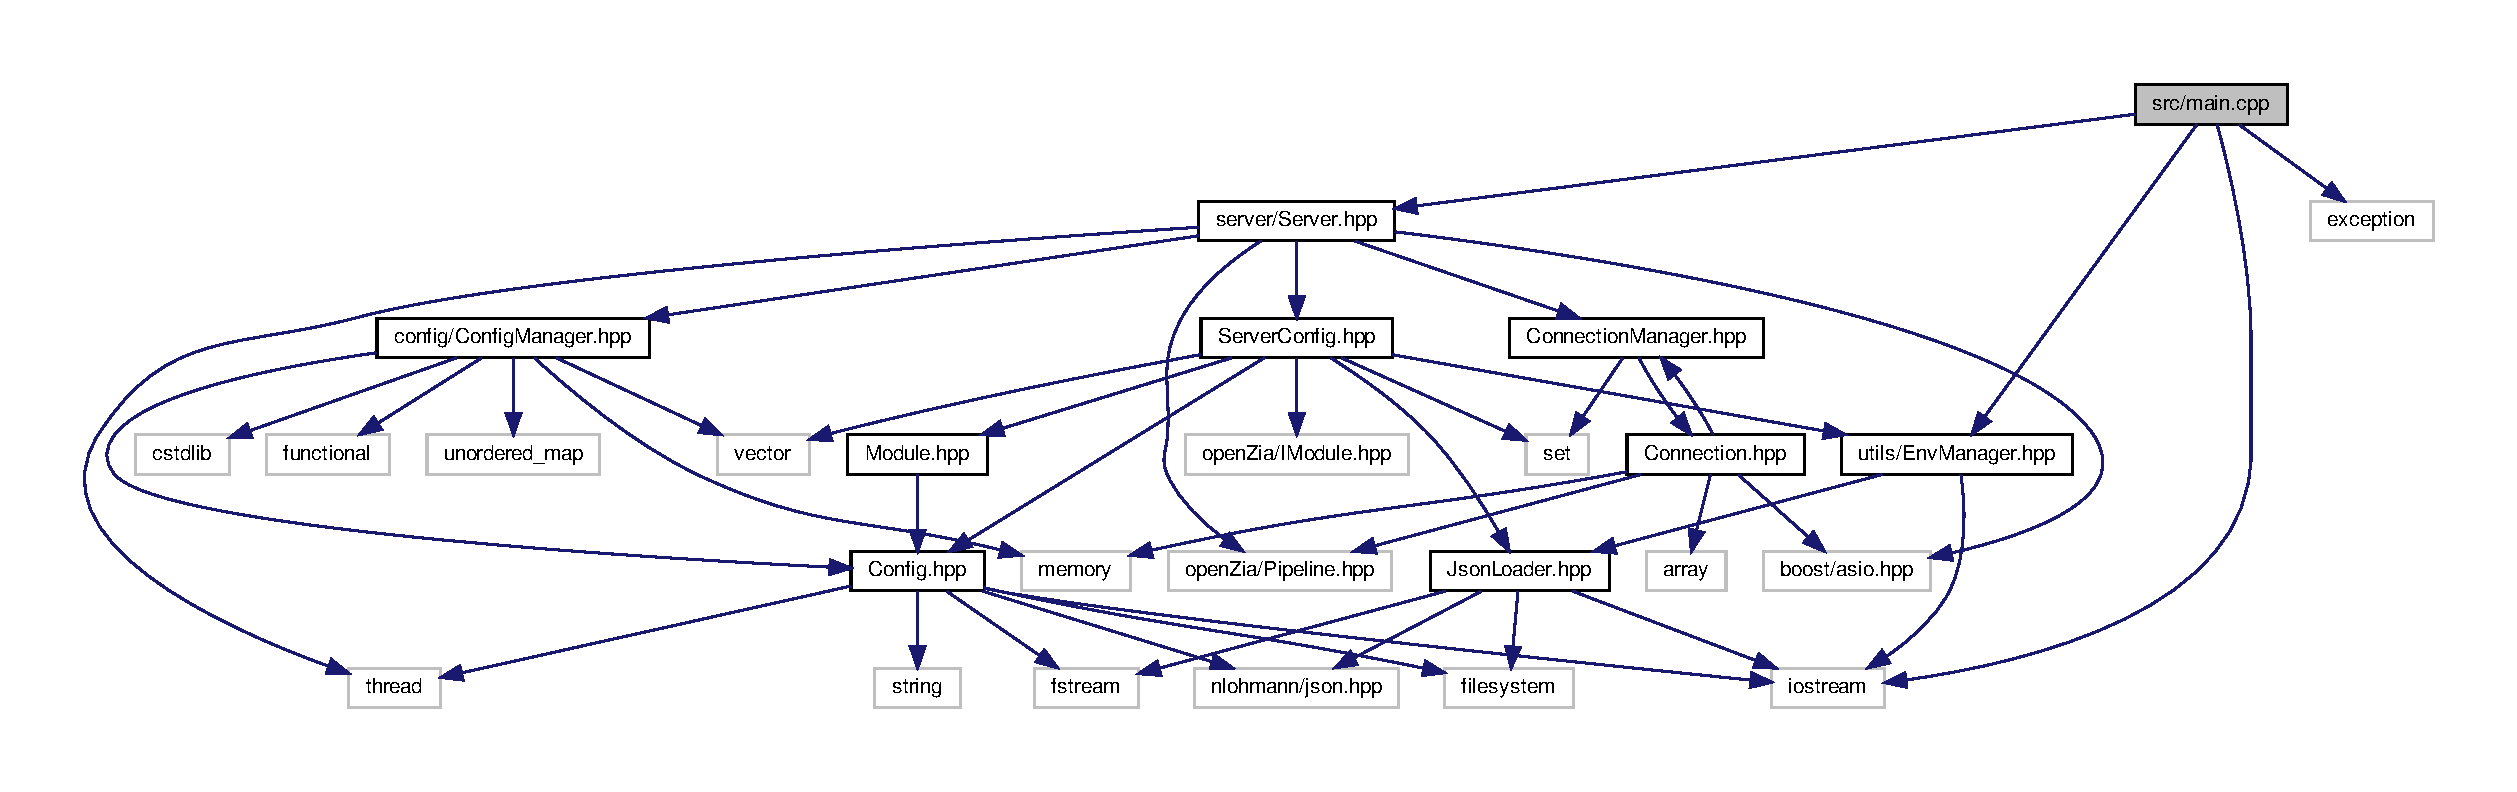
\includegraphics[width=350pt]{main_8cpp__incl}
\end{center}
\end{figure}
\subsection*{Functions}
\begin{DoxyCompactItemize}
\item 
int \hyperlink{main_8cpp_a0ddf1224851353fc92bfbff6f499fa97}{main} (int argc, char $\ast$argv\mbox{[}$\,$\mbox{]})
\end{DoxyCompactItemize}


\subsection{Function Documentation}
\mbox{\Hypertarget{main_8cpp_a0ddf1224851353fc92bfbff6f499fa97}\label{main_8cpp_a0ddf1224851353fc92bfbff6f499fa97}} 
\index{main.\+cpp@{main.\+cpp}!main@{main}}
\index{main@{main}!main.\+cpp@{main.\+cpp}}
\subsubsection{\texorpdfstring{main()}{main()}}
{\footnotesize\ttfamily int main (\begin{DoxyParamCaption}\item[{int}]{argc,  }\item[{char $\ast$}]{argv\mbox{[}$\,$\mbox{]} }\end{DoxyParamCaption})}



Definition at line 33 of file main.\+cpp.


\hypertarget{_fill_page_8cpp}{}\section{src/modules/fill\+Page/\+Fill\+Page.cpp File Reference}
\label{_fill_page_8cpp}\index{src/modules/fill\+Page/\+Fill\+Page.\+cpp@{src/modules/fill\+Page/\+Fill\+Page.\+cpp}}
{\ttfamily \#include $<$string$>$}\newline
{\ttfamily \#include $<$sstream$>$}\newline
{\ttfamily \#include $<$fstream$>$}\newline
{\ttfamily \#include $<$iostream$>$}\newline
{\ttfamily \#include $<$filesystem$>$}\newline
{\ttfamily \#include \char`\"{}Fill\+Page.\+hpp\char`\"{}}\newline
Include dependency graph for Fill\+Page.\+cpp\+:\nopagebreak
\begin{figure}[H]
\begin{center}
\leavevmode
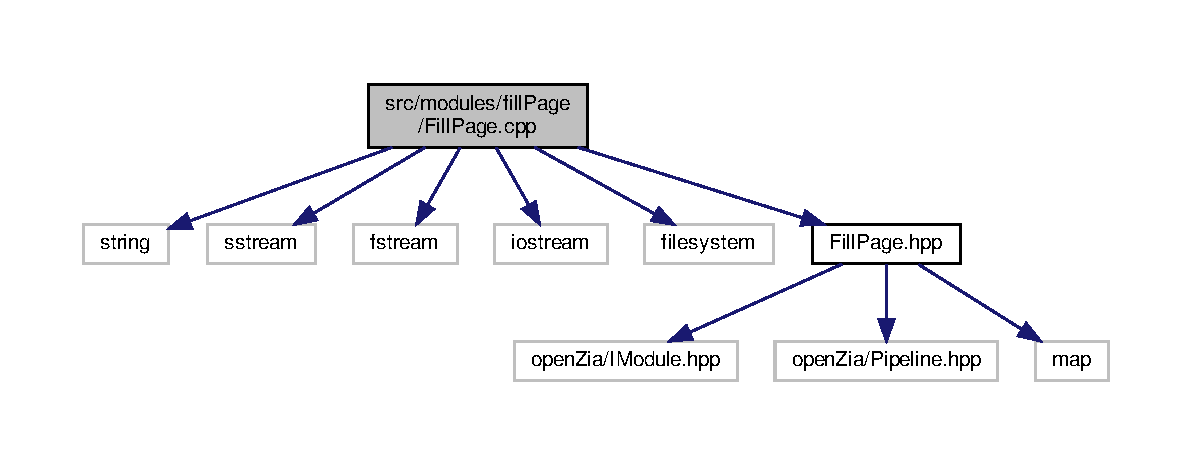
\includegraphics[width=350pt]{_fill_page_8cpp__incl}
\end{center}
\end{figure}

\hypertarget{_fill_page_8hpp}{}\section{src/modules/fill\+Page/\+Fill\+Page.hpp File Reference}
\label{_fill_page_8hpp}\index{src/modules/fill\+Page/\+Fill\+Page.\+hpp@{src/modules/fill\+Page/\+Fill\+Page.\+hpp}}
{\ttfamily \#include $<$open\+Zia/\+I\+Module.\+hpp$>$}\newline
{\ttfamily \#include $<$open\+Zia/\+Pipeline.\+hpp$>$}\newline
{\ttfamily \#include $<$map$>$}\newline
Include dependency graph for Fill\+Page.\+hpp\+:\nopagebreak
\begin{figure}[H]
\begin{center}
\leavevmode
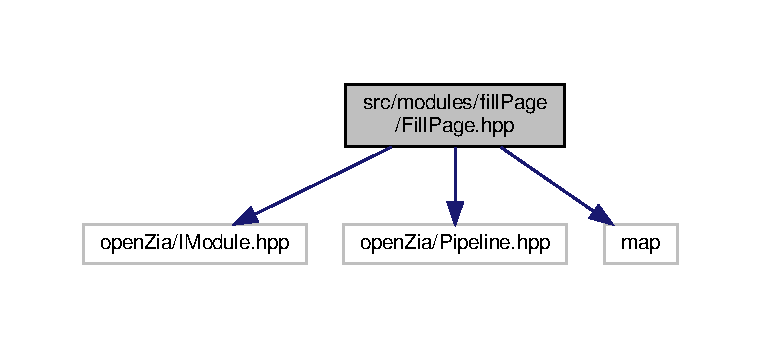
\includegraphics[width=350pt]{_fill_page_8hpp__incl}
\end{center}
\end{figure}
This graph shows which files directly or indirectly include this file\+:\nopagebreak
\begin{figure}[H]
\begin{center}
\leavevmode
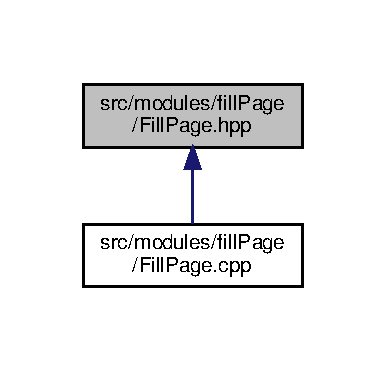
\includegraphics[width=185pt]{_fill_page_8hpp__dep__incl}
\end{center}
\end{figure}
\subsection*{Classes}
\begin{DoxyCompactItemize}
\item 
class \hyperlink{class_fill}{Fill}
\begin{DoxyCompactList}\small\item\em \hyperlink{class_fill}{Fill} class to manage the \hyperlink{class_fill}{Fill} module. \end{DoxyCompactList}\end{DoxyCompactItemize}
\subsection*{Namespaces}
\begin{DoxyCompactItemize}
\item 
 \hyperlink{namespace_fill_module}{Fill\+Module}
\end{DoxyCompactItemize}
\subsection*{Macros}
\begin{DoxyCompactItemize}
\item 
\#define \hyperlink{_fill_page_8hpp_a0eb713c1f5b334a2a612e17a481f09b4}{H\+T\+M\+L\+\_\+\+F\+I\+L\+E\+S\+\_\+\+P\+O\+SI}~\char`\"{}src/H\+T\+ML/\char`\"{}
\item 
\#define \hyperlink{_fill_page_8hpp_abaabb39c497a381da85215fc1ccbdb1a}{H\+T\+M\+L\+\_\+\+F\+I\+L\+E\+\_\+\+E\+R\+R\+OR}~\char`\"{}src/H\+T\+ML/404.html\char`\"{}
\end{DoxyCompactItemize}
\subsection*{Variables}
\begin{DoxyCompactItemize}
\item 
std\+::map$<$ std\+::string, std\+::string $>$ \hyperlink{namespace_fill_module_a3b04872509f930e4a6282619253fb420}{Fill\+Module\+::routes\+\_\+enums}
\begin{DoxyCompactList}\small\item\em Enum for the routes. \end{DoxyCompactList}\item 
std\+::map$<$ std\+::string, std\+::string $>$ \hyperlink{namespace_fill_module_abd8ea40bf0589d3fe6cf7e816164985a}{Fill\+Module\+::formats}
\begin{DoxyCompactList}\small\item\em Enum for the formats. \end{DoxyCompactList}\end{DoxyCompactItemize}


\subsection{Macro Definition Documentation}
\mbox{\Hypertarget{_fill_page_8hpp_abaabb39c497a381da85215fc1ccbdb1a}\label{_fill_page_8hpp_abaabb39c497a381da85215fc1ccbdb1a}} 
\index{Fill\+Page.\+hpp@{Fill\+Page.\+hpp}!H\+T\+M\+L\+\_\+\+F\+I\+L\+E\+\_\+\+E\+R\+R\+OR@{H\+T\+M\+L\+\_\+\+F\+I\+L\+E\+\_\+\+E\+R\+R\+OR}}
\index{H\+T\+M\+L\+\_\+\+F\+I\+L\+E\+\_\+\+E\+R\+R\+OR@{H\+T\+M\+L\+\_\+\+F\+I\+L\+E\+\_\+\+E\+R\+R\+OR}!Fill\+Page.\+hpp@{Fill\+Page.\+hpp}}
\subsubsection{\texorpdfstring{H\+T\+M\+L\+\_\+\+F\+I\+L\+E\+\_\+\+E\+R\+R\+OR}{HTML\_FILE\_ERROR}}
{\footnotesize\ttfamily \#define H\+T\+M\+L\+\_\+\+F\+I\+L\+E\+\_\+\+E\+R\+R\+OR~\char`\"{}src/H\+T\+ML/404.html\char`\"{}}



Definition at line 15 of file Fill\+Page.\+hpp.

\mbox{\Hypertarget{_fill_page_8hpp_a0eb713c1f5b334a2a612e17a481f09b4}\label{_fill_page_8hpp_a0eb713c1f5b334a2a612e17a481f09b4}} 
\index{Fill\+Page.\+hpp@{Fill\+Page.\+hpp}!H\+T\+M\+L\+\_\+\+F\+I\+L\+E\+S\+\_\+\+P\+O\+SI@{H\+T\+M\+L\+\_\+\+F\+I\+L\+E\+S\+\_\+\+P\+O\+SI}}
\index{H\+T\+M\+L\+\_\+\+F\+I\+L\+E\+S\+\_\+\+P\+O\+SI@{H\+T\+M\+L\+\_\+\+F\+I\+L\+E\+S\+\_\+\+P\+O\+SI}!Fill\+Page.\+hpp@{Fill\+Page.\+hpp}}
\subsubsection{\texorpdfstring{H\+T\+M\+L\+\_\+\+F\+I\+L\+E\+S\+\_\+\+P\+O\+SI}{HTML\_FILES\_POSI}}
{\footnotesize\ttfamily \#define H\+T\+M\+L\+\_\+\+F\+I\+L\+E\+S\+\_\+\+P\+O\+SI~\char`\"{}src/H\+T\+ML/\char`\"{}}



Definition at line 14 of file Fill\+Page.\+hpp.


\hypertarget{_parser_module_8cpp}{}\section{src/modules/parser/\+Parser\+Module.cpp File Reference}
\label{_parser_module_8cpp}\index{src/modules/parser/\+Parser\+Module.\+cpp@{src/modules/parser/\+Parser\+Module.\+cpp}}
{\ttfamily \#include $<$string$>$}\newline
{\ttfamily \#include $<$sstream$>$}\newline
{\ttfamily \#include $<$iostream$>$}\newline
{\ttfamily \#include \char`\"{}Parser\+Module.\+hpp\char`\"{}}\newline
Include dependency graph for Parser\+Module.\+cpp\+:\nopagebreak
\begin{figure}[H]
\begin{center}
\leavevmode
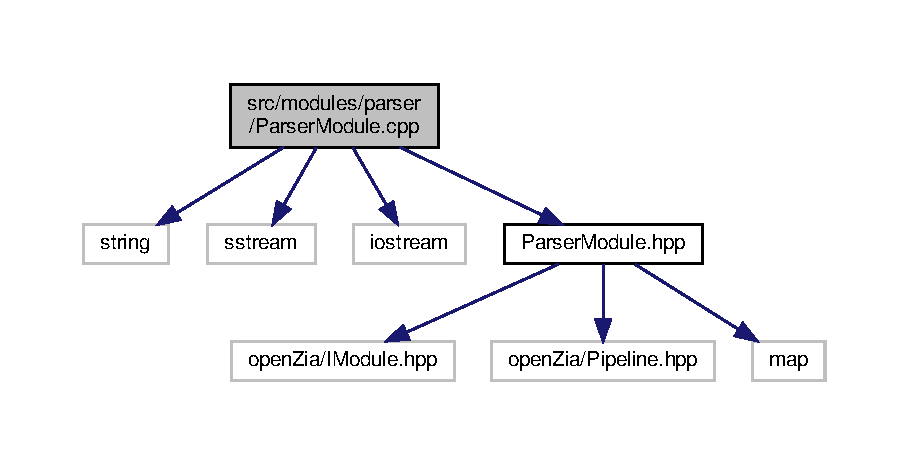
\includegraphics[width=350pt]{_parser_module_8cpp__incl}
\end{center}
\end{figure}

\hypertarget{_parser_module_8hpp}{}\section{src/modules/parser/\+Parser\+Module.hpp File Reference}
\label{_parser_module_8hpp}\index{src/modules/parser/\+Parser\+Module.\+hpp@{src/modules/parser/\+Parser\+Module.\+hpp}}
{\ttfamily \#include $<$open\+Zia/\+I\+Module.\+hpp$>$}\newline
{\ttfamily \#include $<$open\+Zia/\+Pipeline.\+hpp$>$}\newline
{\ttfamily \#include $<$map$>$}\newline
Include dependency graph for Parser\+Module.\+hpp\+:\nopagebreak
\begin{figure}[H]
\begin{center}
\leavevmode
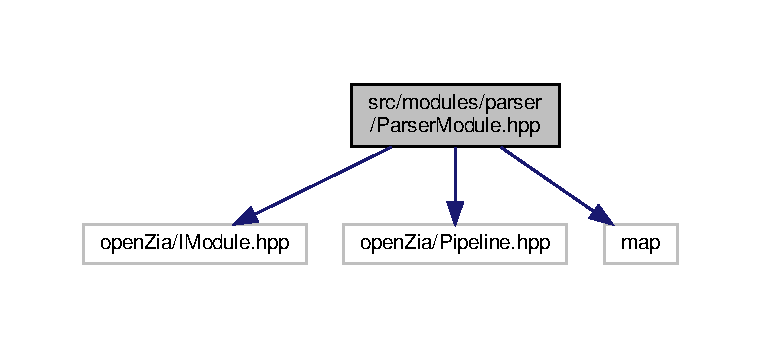
\includegraphics[width=350pt]{_parser_module_8hpp__incl}
\end{center}
\end{figure}
This graph shows which files directly or indirectly include this file\+:\nopagebreak
\begin{figure}[H]
\begin{center}
\leavevmode
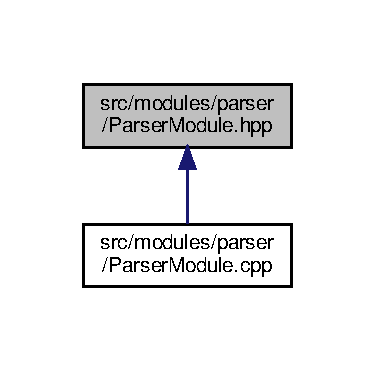
\includegraphics[width=180pt]{_parser_module_8hpp__dep__incl}
\end{center}
\end{figure}
\subsection*{Classes}
\begin{DoxyCompactItemize}
\item 
class \hyperlink{class_parser}{Parser}
\begin{DoxyCompactList}\small\item\em \hyperlink{class_parser}{Parser} class to manage the parser module. \end{DoxyCompactList}\end{DoxyCompactItemize}
\subsection*{Namespaces}
\begin{DoxyCompactItemize}
\item 
 \hyperlink{namespace_parser_module}{Parser\+Module}
\end{DoxyCompactItemize}
\subsection*{Variables}
\begin{DoxyCompactItemize}
\item 
const std\+::vector$<$ std\+::string $>$ \hyperlink{namespace_parser_module_a937e2668b9b022b39ae69bf8169ef491}{Parser\+Module\+::methods}
\begin{DoxyCompactList}\small\item\em Enum for the H\+T\+TP methods. \end{DoxyCompactList}\item 
std\+::map$<$ std\+::string, o\+Z\+::\+H\+T\+T\+P\+::\+Method $>$ \hyperlink{namespace_parser_module_a4a564d139a12507911cf117e50ca1633}{Parser\+Module\+::methods\+\_\+enums}
\begin{DoxyCompactList}\small\item\em Enum between H\+T\+TP method and the api definds. \end{DoxyCompactList}\end{DoxyCompactItemize}

\hypertarget{_p_h_p_module_8cpp}{}\section{src/modules/\+P\+H\+P/\+P\+H\+P\+Module.cpp File Reference}
\label{_p_h_p_module_8cpp}\index{src/modules/\+P\+H\+P/\+P\+H\+P\+Module.\+cpp@{src/modules/\+P\+H\+P/\+P\+H\+P\+Module.\+cpp}}
{\ttfamily \#include \char`\"{}P\+H\+P\+Module.\+hpp\char`\"{}}\newline
{\ttfamily \#include $<$cstdlib$>$}\newline
Include dependency graph for P\+H\+P\+Module.\+cpp\+:\nopagebreak
\begin{figure}[H]
\begin{center}
\leavevmode
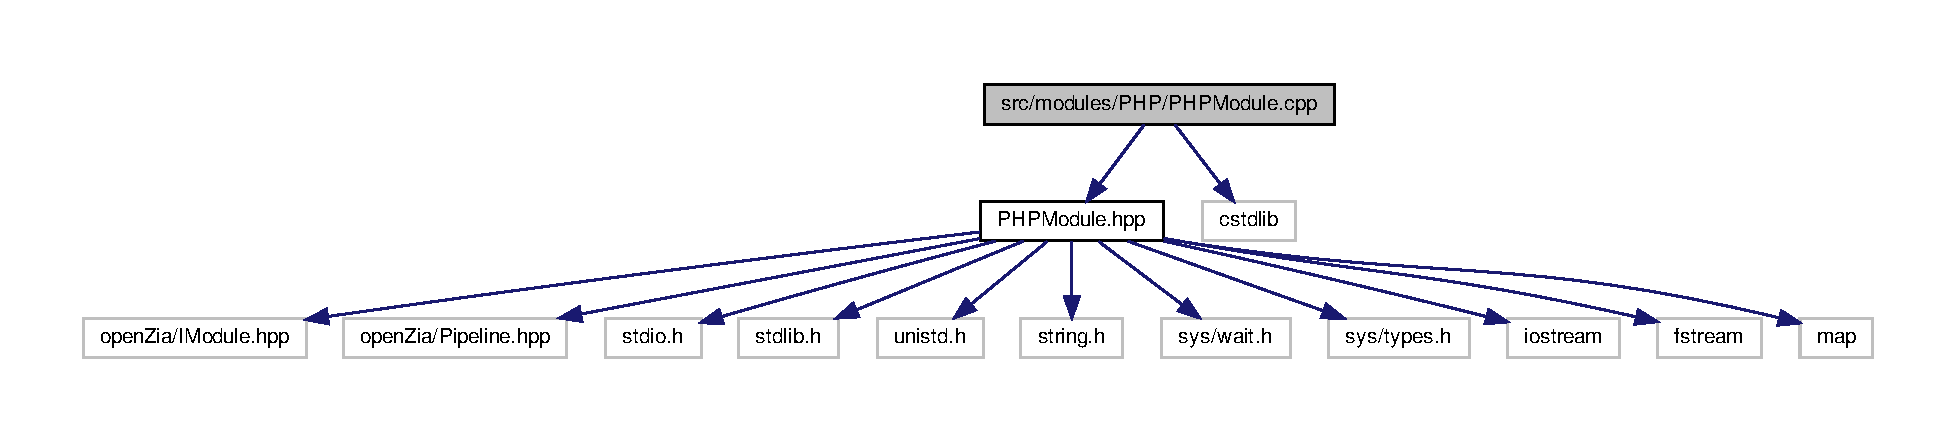
\includegraphics[width=350pt]{_p_h_p_module_8cpp__incl}
\end{center}
\end{figure}

\hypertarget{_p_h_p_module_8hpp}{}\section{src/modules/\+P\+H\+P/\+P\+H\+P\+Module.hpp File Reference}
\label{_p_h_p_module_8hpp}\index{src/modules/\+P\+H\+P/\+P\+H\+P\+Module.\+hpp@{src/modules/\+P\+H\+P/\+P\+H\+P\+Module.\+hpp}}
{\ttfamily \#include $<$open\+Zia/\+I\+Module.\+hpp$>$}\newline
{\ttfamily \#include $<$open\+Zia/\+Pipeline.\+hpp$>$}\newline
{\ttfamily \#include $<$stdio.\+h$>$}\newline
{\ttfamily \#include $<$stdlib.\+h$>$}\newline
{\ttfamily \#include $<$unistd.\+h$>$}\newline
{\ttfamily \#include $<$string.\+h$>$}\newline
{\ttfamily \#include $<$sys/wait.\+h$>$}\newline
{\ttfamily \#include $<$sys/types.\+h$>$}\newline
{\ttfamily \#include $<$iostream$>$}\newline
{\ttfamily \#include $<$fstream$>$}\newline
{\ttfamily \#include $<$map$>$}\newline
Include dependency graph for P\+H\+P\+Module.\+hpp\+:\nopagebreak
\begin{figure}[H]
\begin{center}
\leavevmode
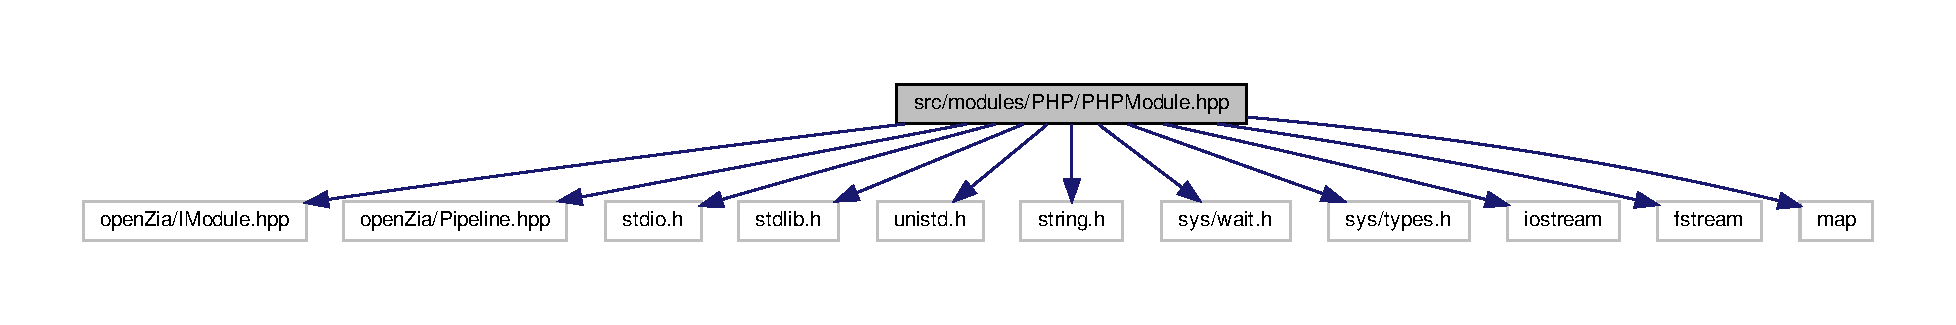
\includegraphics[width=350pt]{_p_h_p_module_8hpp__incl}
\end{center}
\end{figure}
This graph shows which files directly or indirectly include this file\+:\nopagebreak
\begin{figure}[H]
\begin{center}
\leavevmode
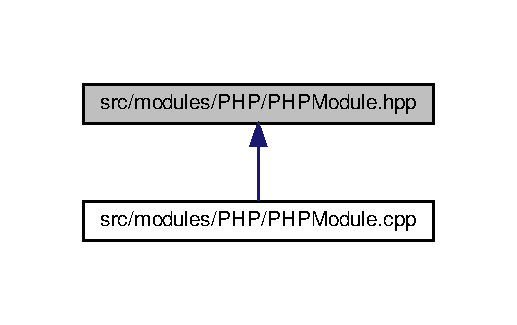
\includegraphics[width=248pt]{_p_h_p_module_8hpp__dep__incl}
\end{center}
\end{figure}
\subsection*{Classes}
\begin{DoxyCompactItemize}
\item 
class \hyperlink{class_p_h_p___c_g_i}{P\+H\+P\+\_\+\+C\+GI}
\begin{DoxyCompactList}\small\item\em \hyperlink{class_p_h_p___c_g_i}{P\+H\+P\+\_\+\+C\+GI} class to manage the P\+HP module. \end{DoxyCompactList}\end{DoxyCompactItemize}
\subsection*{Namespaces}
\begin{DoxyCompactItemize}
\item 
 \hyperlink{namespace_p_h_p_module}{P\+H\+P\+Module}
\end{DoxyCompactItemize}
\subsection*{Macros}
\begin{DoxyCompactItemize}
\item 
\#define \hyperlink{_p_h_p_module_8hpp_a0eb713c1f5b334a2a612e17a481f09b4}{H\+T\+M\+L\+\_\+\+F\+I\+L\+E\+S\+\_\+\+P\+O\+SI}~\char`\"{}src/H\+T\+ML/\char`\"{}
\end{DoxyCompactItemize}
\subsection*{Variables}
\begin{DoxyCompactItemize}
\item 
std\+::map$<$ std\+::string, std\+::string $>$ \hyperlink{namespace_p_h_p_module_a8b51dfcb9114f032151ac407675938b1}{P\+H\+P\+Module\+::routes\+\_\+enums}
\begin{DoxyCompactList}\small\item\em Enum for the server\textquotesingle{}s routes with php. \end{DoxyCompactList}\end{DoxyCompactItemize}


\subsection{Macro Definition Documentation}
\mbox{\Hypertarget{_p_h_p_module_8hpp_a0eb713c1f5b334a2a612e17a481f09b4}\label{_p_h_p_module_8hpp_a0eb713c1f5b334a2a612e17a481f09b4}} 
\index{P\+H\+P\+Module.\+hpp@{P\+H\+P\+Module.\+hpp}!H\+T\+M\+L\+\_\+\+F\+I\+L\+E\+S\+\_\+\+P\+O\+SI@{H\+T\+M\+L\+\_\+\+F\+I\+L\+E\+S\+\_\+\+P\+O\+SI}}
\index{H\+T\+M\+L\+\_\+\+F\+I\+L\+E\+S\+\_\+\+P\+O\+SI@{H\+T\+M\+L\+\_\+\+F\+I\+L\+E\+S\+\_\+\+P\+O\+SI}!P\+H\+P\+Module.\+hpp@{P\+H\+P\+Module.\+hpp}}
\subsubsection{\texorpdfstring{H\+T\+M\+L\+\_\+\+F\+I\+L\+E\+S\+\_\+\+P\+O\+SI}{HTML\_FILES\_POSI}}
{\footnotesize\ttfamily \#define H\+T\+M\+L\+\_\+\+F\+I\+L\+E\+S\+\_\+\+P\+O\+SI~\char`\"{}src/H\+T\+ML/\char`\"{}}



Definition at line 22 of file P\+H\+P\+Module.\+hpp.


\hypertarget{_s_s_l_module_8cpp}{}\section{src/modules/\+S\+S\+L/\+S\+S\+L\+Module.cpp File Reference}
\label{_s_s_l_module_8cpp}\index{src/modules/\+S\+S\+L/\+S\+S\+L\+Module.\+cpp@{src/modules/\+S\+S\+L/\+S\+S\+L\+Module.\+cpp}}
{\ttfamily \#include \char`\"{}S\+S\+L\+Module.\+hpp\char`\"{}}\newline
Include dependency graph for S\+S\+L\+Module.\+cpp\+:\nopagebreak
\begin{figure}[H]
\begin{center}
\leavevmode
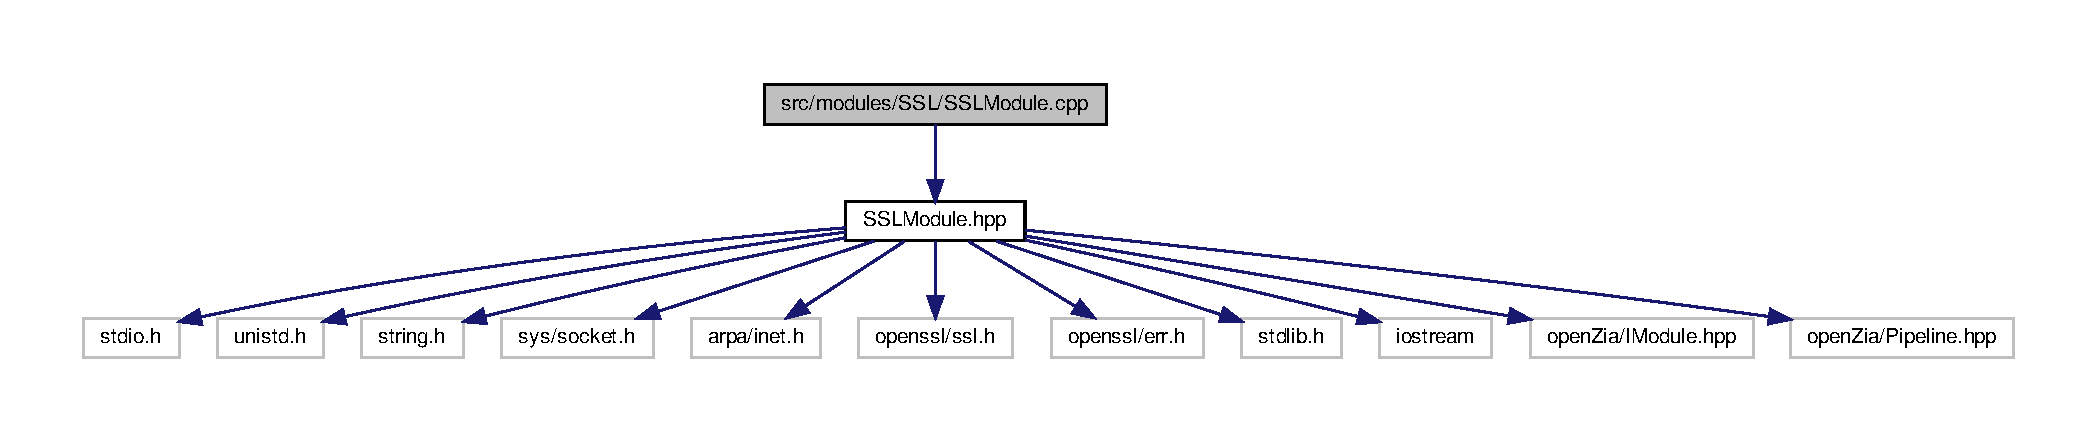
\includegraphics[width=350pt]{_s_s_l_module_8cpp__incl}
\end{center}
\end{figure}

\hypertarget{_s_s_l_module_8hpp}{}\section{src/modules/\+S\+S\+L/\+S\+S\+L\+Module.hpp File Reference}
\label{_s_s_l_module_8hpp}\index{src/modules/\+S\+S\+L/\+S\+S\+L\+Module.\+hpp@{src/modules/\+S\+S\+L/\+S\+S\+L\+Module.\+hpp}}
{\ttfamily \#include $<$stdio.\+h$>$}\newline
{\ttfamily \#include $<$unistd.\+h$>$}\newline
{\ttfamily \#include $<$string.\+h$>$}\newline
{\ttfamily \#include $<$sys/socket.\+h$>$}\newline
{\ttfamily \#include $<$arpa/inet.\+h$>$}\newline
{\ttfamily \#include $<$openssl/ssl.\+h$>$}\newline
{\ttfamily \#include $<$openssl/err.\+h$>$}\newline
{\ttfamily \#include $<$stdlib.\+h$>$}\newline
{\ttfamily \#include $<$iostream$>$}\newline
{\ttfamily \#include $<$open\+Zia/\+I\+Module.\+hpp$>$}\newline
{\ttfamily \#include $<$open\+Zia/\+Pipeline.\+hpp$>$}\newline
Include dependency graph for S\+S\+L\+Module.\+hpp\+:\nopagebreak
\begin{figure}[H]
\begin{center}
\leavevmode
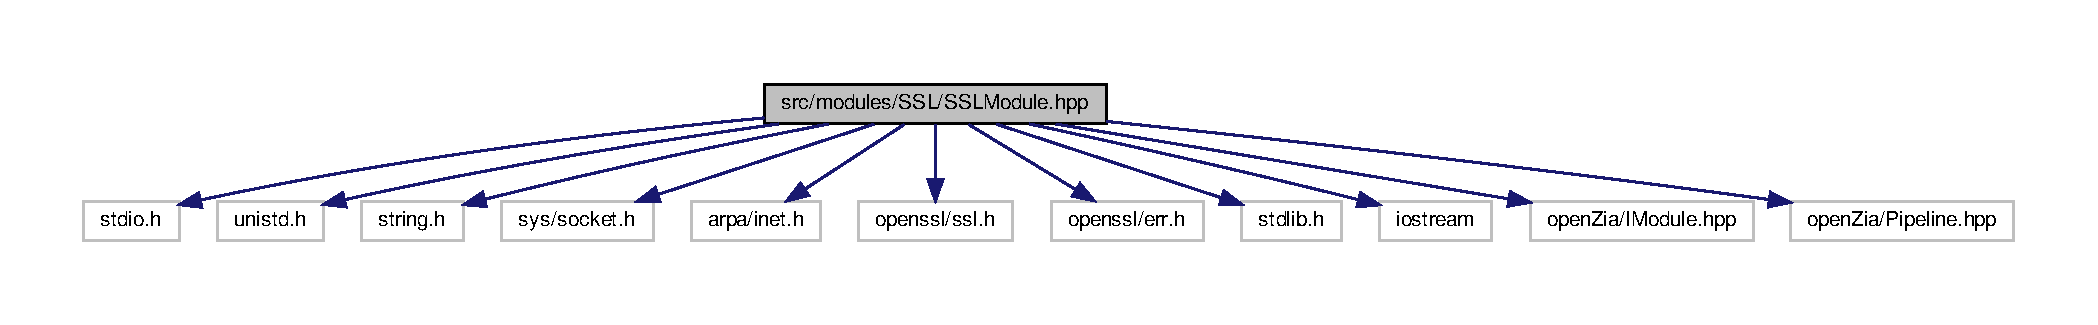
\includegraphics[width=350pt]{_s_s_l_module_8hpp__incl}
\end{center}
\end{figure}
This graph shows which files directly or indirectly include this file\+:\nopagebreak
\begin{figure}[H]
\begin{center}
\leavevmode
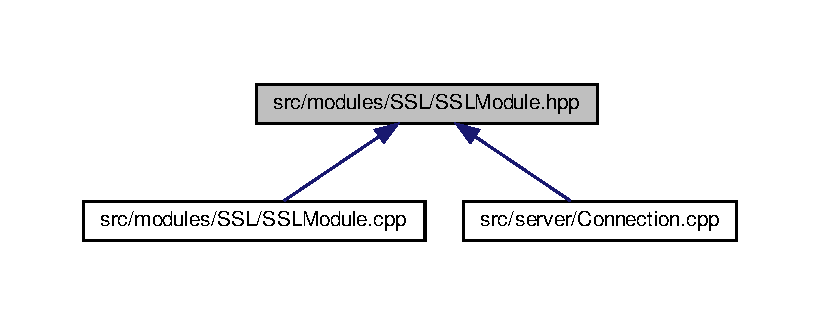
\includegraphics[width=350pt]{_s_s_l_module_8hpp__dep__incl}
\end{center}
\end{figure}
\subsection*{Classes}
\begin{DoxyCompactItemize}
\item 
class \hyperlink{class_s_s_l_module}{S\+S\+L\+Module}
\begin{DoxyCompactList}\small\item\em \hyperlink{class_s_s_l_module}{S\+S\+L\+Module} class to manage the S\+SL module. \end{DoxyCompactList}\end{DoxyCompactItemize}

\hypertarget{_connection_8cpp}{}\section{src/server/\+Connection.cpp File Reference}
\label{_connection_8cpp}\index{src/server/\+Connection.\+cpp@{src/server/\+Connection.\+cpp}}
{\ttfamily \#include $<$iostream$>$}\newline
{\ttfamily \#include $<$vector$>$}\newline
{\ttfamily \#include $<$iterator$>$}\newline
{\ttfamily \#include $<$array$>$}\newline
{\ttfamily \#include $<$utility$>$}\newline
{\ttfamily \#include \char`\"{}Connection.\+hpp\char`\"{}}\newline
{\ttfamily \#include \char`\"{}Log.\+hpp\char`\"{}}\newline
{\ttfamily \#include $<$modules/\+S\+S\+L/\+S\+S\+L\+Module.\+hpp$>$}\newline
Include dependency graph for Connection.\+cpp\+:\nopagebreak
\begin{figure}[H]
\begin{center}
\leavevmode
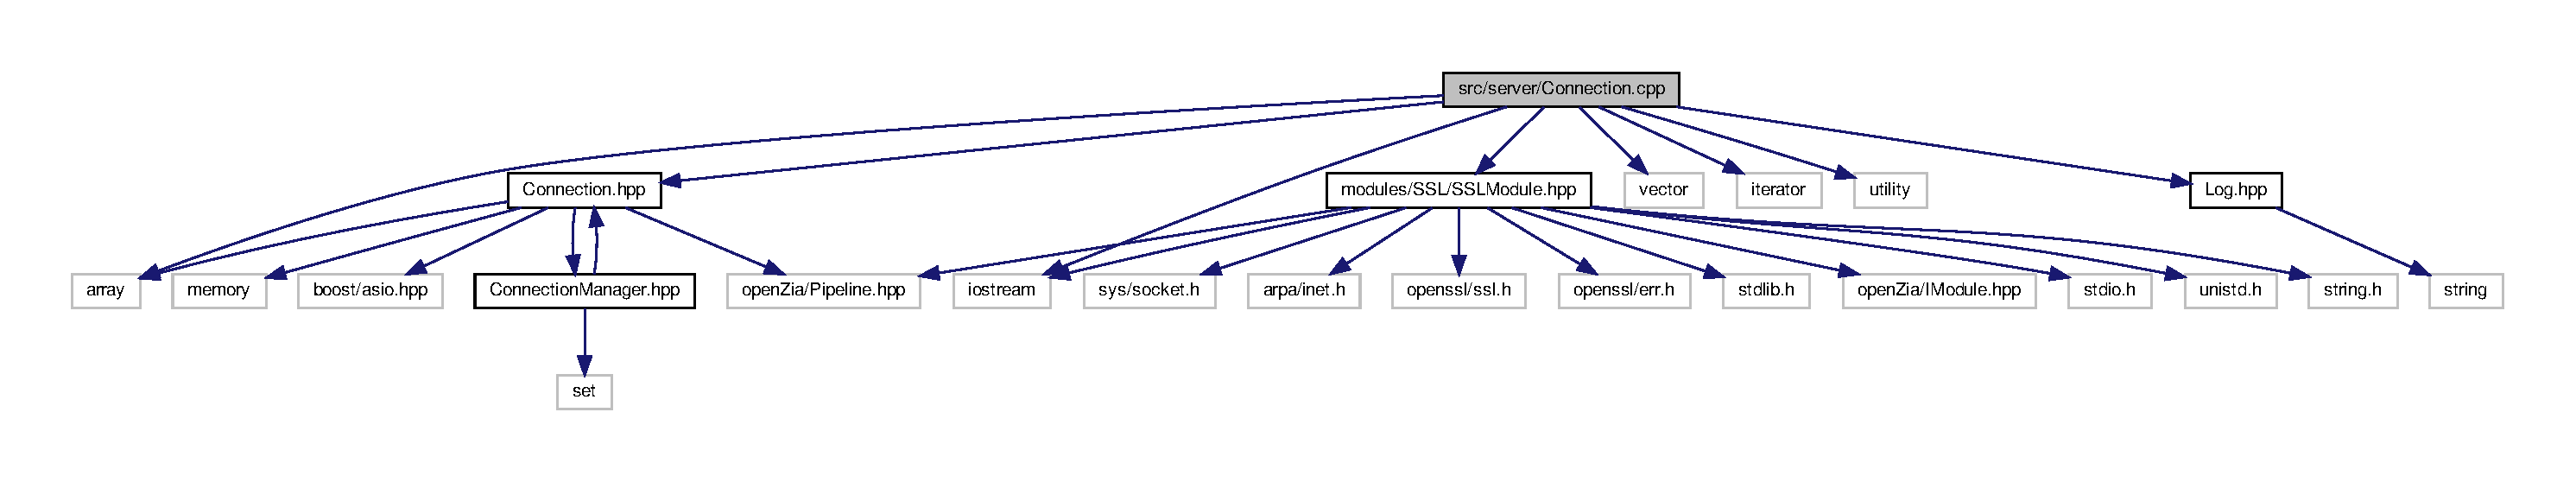
\includegraphics[width=350pt]{_connection_8cpp__incl}
\end{center}
\end{figure}

\hypertarget{_connection_8hpp}{}\section{src/server/\+Connection.hpp File Reference}
\label{_connection_8hpp}\index{src/server/\+Connection.\+hpp@{src/server/\+Connection.\+hpp}}
{\ttfamily \#include $<$array$>$}\newline
{\ttfamily \#include $<$memory$>$}\newline
{\ttfamily \#include $<$boost/asio.\+hpp$>$}\newline
{\ttfamily \#include \char`\"{}open\+Zia/\+Pipeline.\+hpp\char`\"{}}\newline
{\ttfamily \#include \char`\"{}Connection\+Manager.\+hpp\char`\"{}}\newline
Include dependency graph for Connection.\+hpp\+:\nopagebreak
\begin{figure}[H]
\begin{center}
\leavevmode
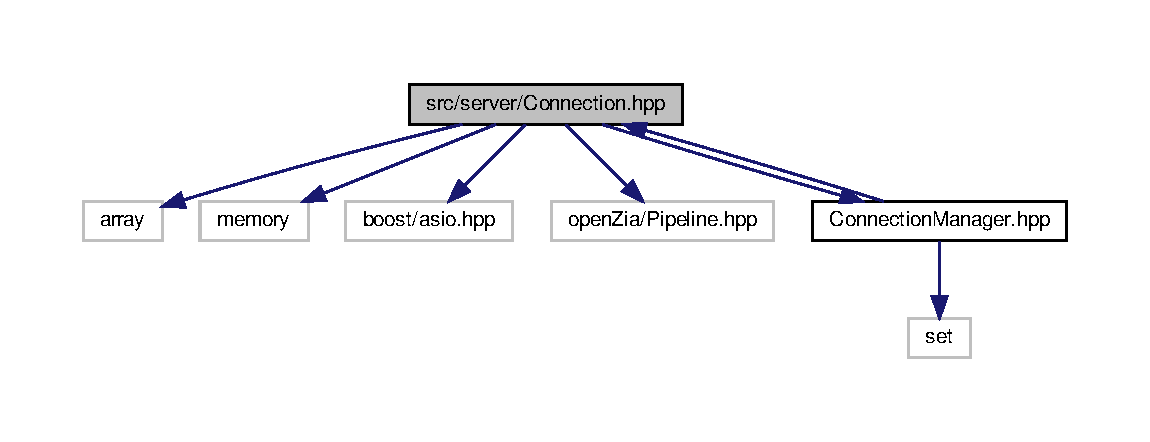
\includegraphics[width=350pt]{_connection_8hpp__incl}
\end{center}
\end{figure}
This graph shows which files directly or indirectly include this file\+:\nopagebreak
\begin{figure}[H]
\begin{center}
\leavevmode
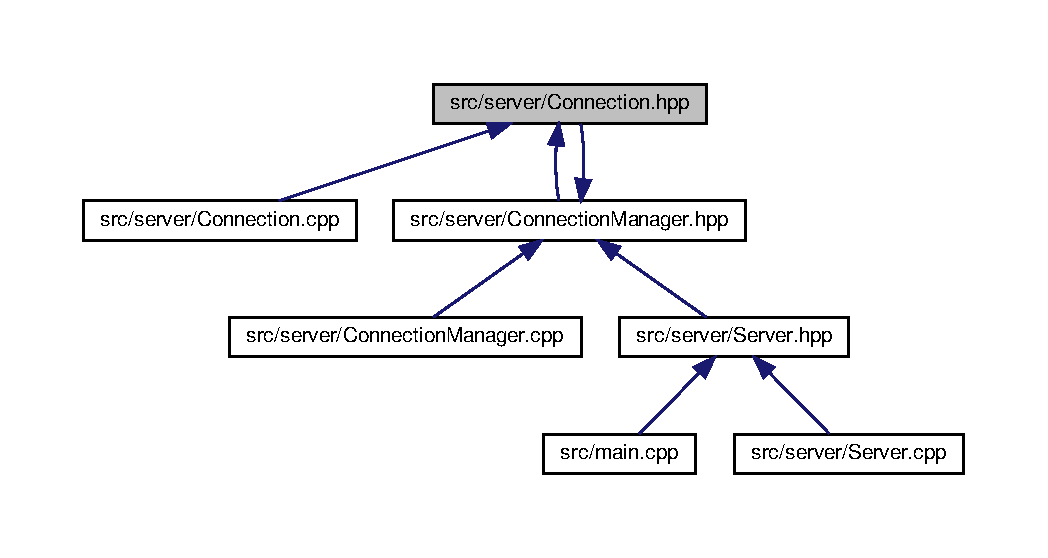
\includegraphics[width=350pt]{_connection_8hpp__dep__incl}
\end{center}
\end{figure}
\subsection*{Classes}
\begin{DoxyCompactItemize}
\item 
class \hyperlink{class_zia_1_1_connection}{Zia\+::\+Connection}
\begin{DoxyCompactList}\small\item\em \hyperlink{class_zia_1_1_connection}{Connection} class to manage the connection. \end{DoxyCompactList}\end{DoxyCompactItemize}
\subsection*{Namespaces}
\begin{DoxyCompactItemize}
\item 
 \hyperlink{namespace_zia}{Zia}
\end{DoxyCompactItemize}

\hypertarget{_connection_manager_8cpp}{}\section{src/server/\+Connection\+Manager.cpp File Reference}
\label{_connection_manager_8cpp}\index{src/server/\+Connection\+Manager.\+cpp@{src/server/\+Connection\+Manager.\+cpp}}
{\ttfamily \#include \char`\"{}Connection\+Manager.\+hpp\char`\"{}}\newline
{\ttfamily \#include $<$iostream$>$}\newline
Include dependency graph for Connection\+Manager.\+cpp\+:\nopagebreak
\begin{figure}[H]
\begin{center}
\leavevmode
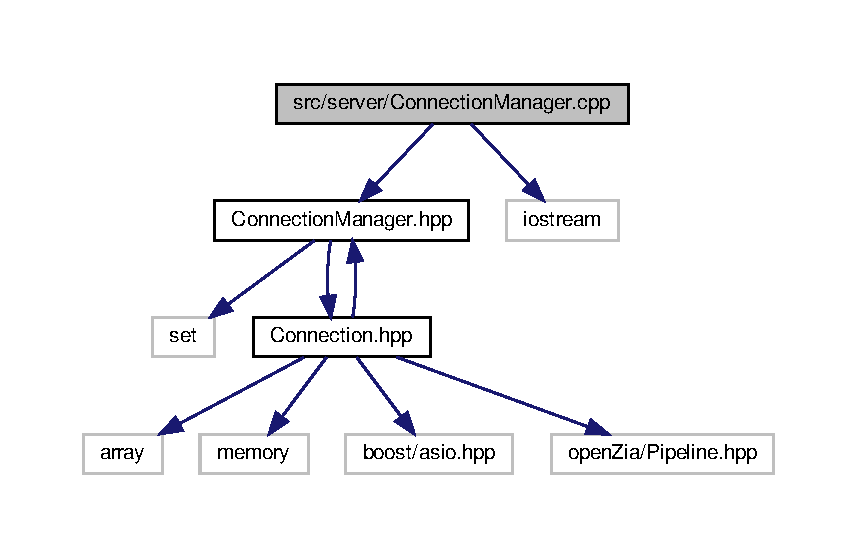
\includegraphics[width=350pt]{_connection_manager_8cpp__incl}
\end{center}
\end{figure}

\hypertarget{_connection_manager_8hpp}{}\section{src/server/\+Connection\+Manager.hpp File Reference}
\label{_connection_manager_8hpp}\index{src/server/\+Connection\+Manager.\+hpp@{src/server/\+Connection\+Manager.\+hpp}}
{\ttfamily \#include $<$set$>$}\newline
{\ttfamily \#include \char`\"{}Connection.\+hpp\char`\"{}}\newline
Include dependency graph for Connection\+Manager.\+hpp\+:\nopagebreak
\begin{figure}[H]
\begin{center}
\leavevmode
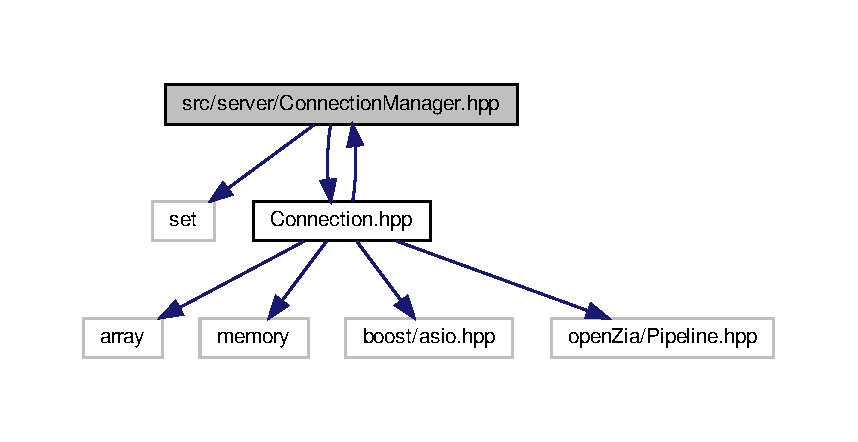
\includegraphics[width=350pt]{_connection_manager_8hpp__incl}
\end{center}
\end{figure}
This graph shows which files directly or indirectly include this file\+:\nopagebreak
\begin{figure}[H]
\begin{center}
\leavevmode
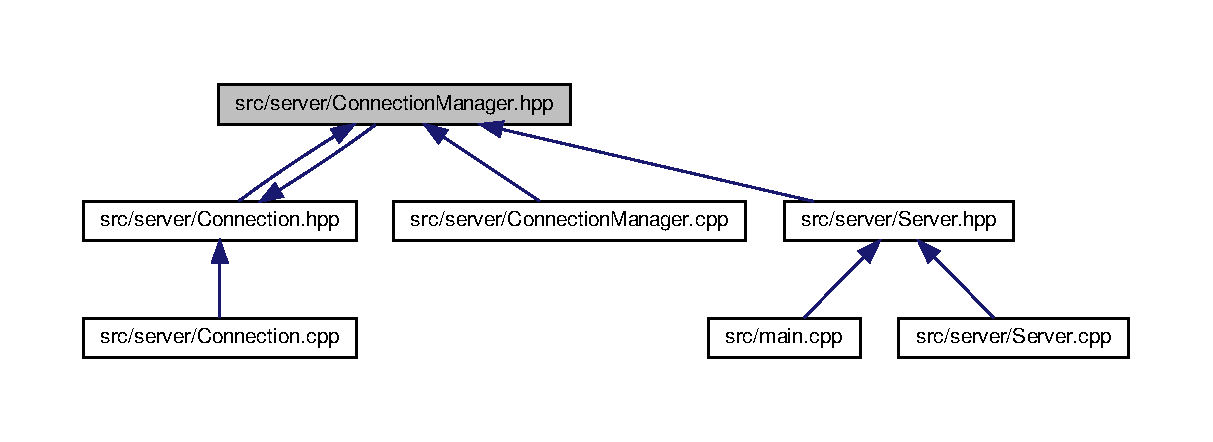
\includegraphics[width=350pt]{_connection_manager_8hpp__dep__incl}
\end{center}
\end{figure}
\subsection*{Classes}
\begin{DoxyCompactItemize}
\item 
class \hyperlink{class_zia_1_1_connection_manager}{Zia\+::\+Connection\+Manager}
\begin{DoxyCompactList}\small\item\em \hyperlink{class_zia_1_1_connection_manager}{Connection\+Manager} class to manage the connection. \end{DoxyCompactList}\end{DoxyCompactItemize}
\subsection*{Namespaces}
\begin{DoxyCompactItemize}
\item 
 \hyperlink{namespace_zia}{Zia}
\end{DoxyCompactItemize}
\subsection*{Typedefs}
\begin{DoxyCompactItemize}
\item 
typedef std\+::shared\+\_\+ptr$<$ \hyperlink{class_zia_1_1_connection}{Zia\+::\+Connection} $>$ \hyperlink{_connection_manager_8hpp_a0e374529952c927bd9f59c9acbccf624}{Connection\+Ptr}
\end{DoxyCompactItemize}


\subsection{Typedef Documentation}
\mbox{\Hypertarget{_connection_manager_8hpp_a0e374529952c927bd9f59c9acbccf624}\label{_connection_manager_8hpp_a0e374529952c927bd9f59c9acbccf624}} 
\index{Connection\+Manager.\+hpp@{Connection\+Manager.\+hpp}!Connection\+Ptr@{Connection\+Ptr}}
\index{Connection\+Ptr@{Connection\+Ptr}!Connection\+Manager.\+hpp@{Connection\+Manager.\+hpp}}
\subsubsection{\texorpdfstring{Connection\+Ptr}{ConnectionPtr}}
{\footnotesize\ttfamily typedef std\+::shared\+\_\+ptr$<$\hyperlink{class_zia_1_1_connection}{Zia\+::\+Connection}$>$ \hyperlink{_connection_manager_8hpp_a0e374529952c927bd9f59c9acbccf624}{Connection\+Ptr}}



Definition at line 19 of file Connection\+Manager.\+hpp.


\hypertarget{_log_8cpp}{}\section{src/server/\+Log.cpp File Reference}
\label{_log_8cpp}\index{src/server/\+Log.\+cpp@{src/server/\+Log.\+cpp}}
{\ttfamily \#include \char`\"{}Log.\+hpp\char`\"{}}\newline
{\ttfamily \#include $<$iomanip$>$}\newline
{\ttfamily \#include $<$iostream$>$}\newline
Include dependency graph for Log.\+cpp\+:\nopagebreak
\begin{figure}[H]
\begin{center}
\leavevmode
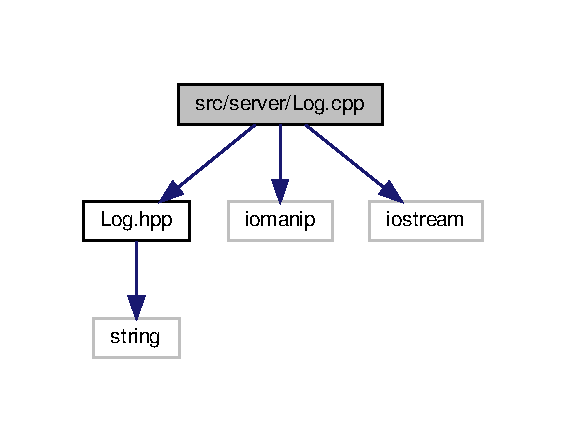
\includegraphics[width=272pt]{_log_8cpp__incl}
\end{center}
\end{figure}

\hypertarget{_log_8hpp}{}\section{/home/mmoinvaziri/\+Epitech/\+C\+P\+P\+\_\+zia\+\_\+2019/\+External/open\+Zia/open\+Zia/\+Log.hpp File Reference}
\label{_log_8hpp}\index{/home/mmoinvaziri/Epitech/CPP\_zia\_2019/External/openZia/openZia/Log.hpp@{/home/mmoinvaziri/Epitech/CPP\_zia\_2019/External/openZia/openZia/Log.hpp}}
{\ttfamily \#include $<$sstream$>$}\newline
{\ttfamily \#include \char`\"{}I\+Logger.\+hpp\char`\"{}}\newline
{\ttfamily \#include \char`\"{}Log.\+ipp\char`\"{}}\newline
\subsection*{Classes}
\begin{DoxyCompactItemize}
\item 
class \mbox{\hyperlink{classo_z_1_1_log}{o\+Z\+::\+Log}}
\end{DoxyCompactItemize}
\subsection*{Namespaces}
\begin{DoxyCompactItemize}
\item 
 \mbox{\hyperlink{namespaceo_z}{oZ}}
\end{DoxyCompactItemize}

\hypertarget{_module_8cpp}{}\section{src/server/\+Module.cpp File Reference}
\label{_module_8cpp}\index{src/server/\+Module.\+cpp@{src/server/\+Module.\+cpp}}
{\ttfamily \#include \char`\"{}Module.\+hpp\char`\"{}}\newline
Include dependency graph for Module.\+cpp\+:\nopagebreak
\begin{figure}[H]
\begin{center}
\leavevmode
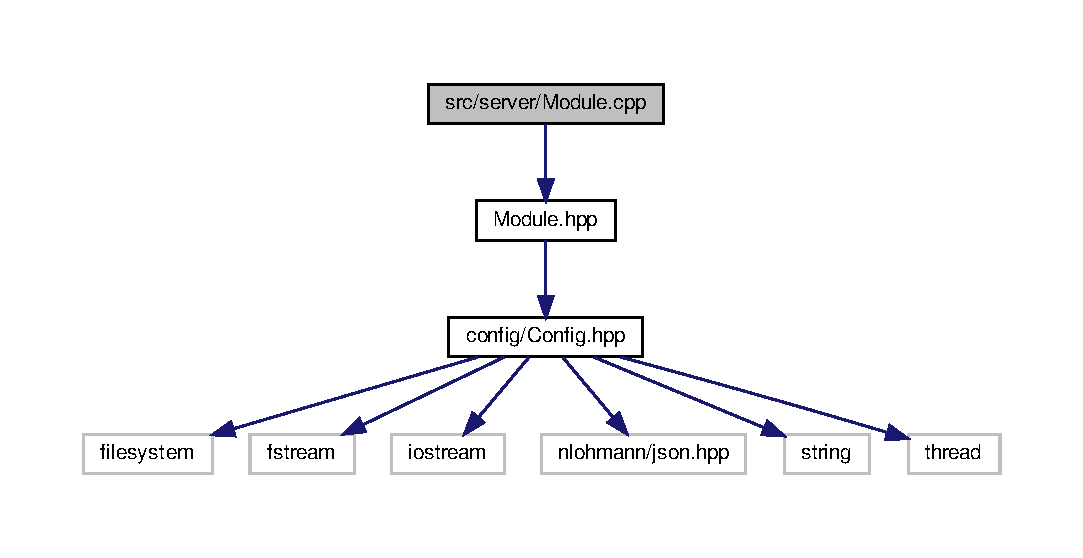
\includegraphics[width=350pt]{_module_8cpp__incl}
\end{center}
\end{figure}

\hypertarget{_module_8hpp}{}\section{src/server/\+Module.hpp File Reference}
\label{_module_8hpp}\index{src/server/\+Module.\+hpp@{src/server/\+Module.\+hpp}}
{\ttfamily \#include $<$config/\+Config.\+hpp$>$}\newline
Include dependency graph for Module.\+hpp\+:\nopagebreak
\begin{figure}[H]
\begin{center}
\leavevmode
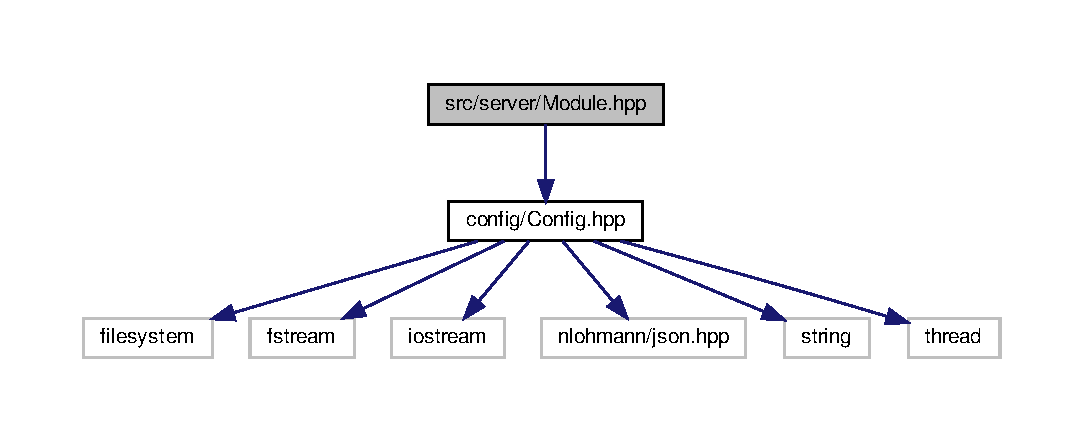
\includegraphics[width=350pt]{_module_8hpp__incl}
\end{center}
\end{figure}
This graph shows which files directly or indirectly include this file\+:\nopagebreak
\begin{figure}[H]
\begin{center}
\leavevmode
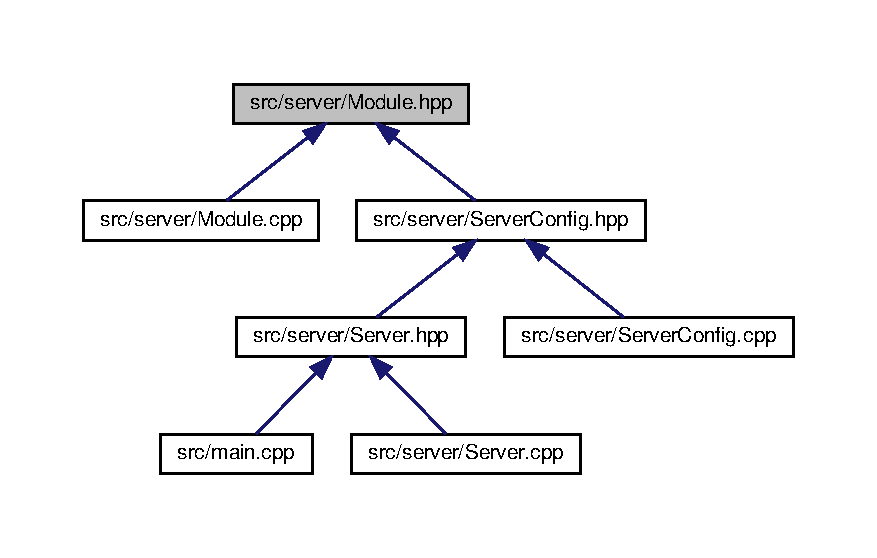
\includegraphics[width=350pt]{_module_8hpp__dep__incl}
\end{center}
\end{figure}
\subsection*{Classes}
\begin{DoxyCompactItemize}
\item 
class \hyperlink{class_zia_1_1_module}{Zia\+::\+Module}
\begin{DoxyCompactList}\small\item\em \hyperlink{class_zia_1_1_module}{Module} class to manage the modules. \end{DoxyCompactList}\end{DoxyCompactItemize}
\subsection*{Namespaces}
\begin{DoxyCompactItemize}
\item 
 \hyperlink{namespace_zia}{Zia}
\end{DoxyCompactItemize}

\hypertarget{_server_8cpp}{}\section{src/server/\+Server.cpp File Reference}
\label{_server_8cpp}\index{src/server/\+Server.\+cpp@{src/server/\+Server.\+cpp}}
{\ttfamily \#include $<$iostream$>$}\newline
{\ttfamily \#include \char`\"{}Server.\+hpp\char`\"{}}\newline
{\ttfamily \#include \char`\"{}Log.\+hpp\char`\"{}}\newline
{\ttfamily \#include $<$boost/asio.\+hpp$>$}\newline
{\ttfamily \#include $<$vector$>$}\newline
{\ttfamily \#include $<$iterator$>$}\newline
Include dependency graph for Server.\+cpp\+:\nopagebreak
\begin{figure}[H]
\begin{center}
\leavevmode
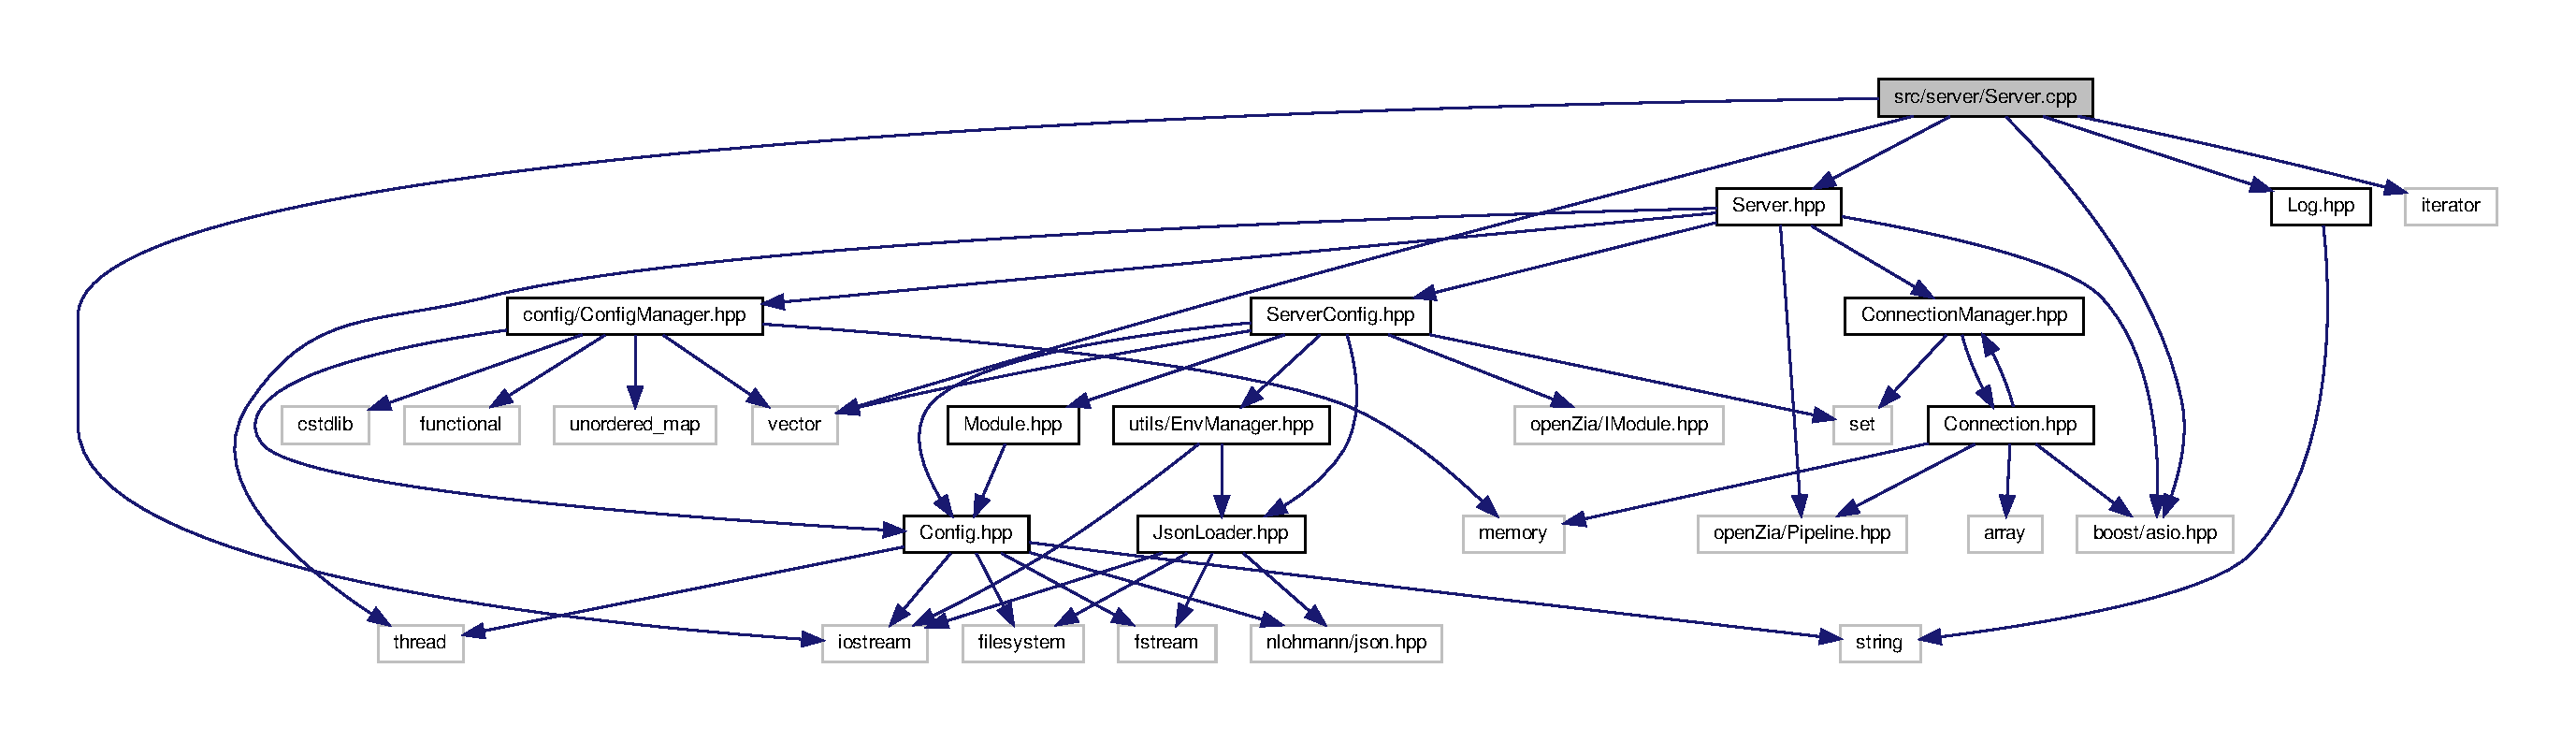
\includegraphics[width=350pt]{_server_8cpp__incl}
\end{center}
\end{figure}

\hypertarget{_server_8hpp}{}\section{src/server/\+Server.hpp File Reference}
\label{_server_8hpp}\index{src/server/\+Server.\+hpp@{src/server/\+Server.\+hpp}}
{\ttfamily \#include $<$thread$>$}\newline
{\ttfamily \#include $<$boost/asio.\+hpp$>$}\newline
{\ttfamily \#include $<$open\+Zia/\+Pipeline.\+hpp$>$}\newline
{\ttfamily \#include $<$config/\+Config\+Manager.\+hpp$>$}\newline
{\ttfamily \#include \char`\"{}Connection\+Manager.\+hpp\char`\"{}}\newline
{\ttfamily \#include \char`\"{}Server\+Config.\+hpp\char`\"{}}\newline
Include dependency graph for Server.\+hpp\+:\nopagebreak
\begin{figure}[H]
\begin{center}
\leavevmode
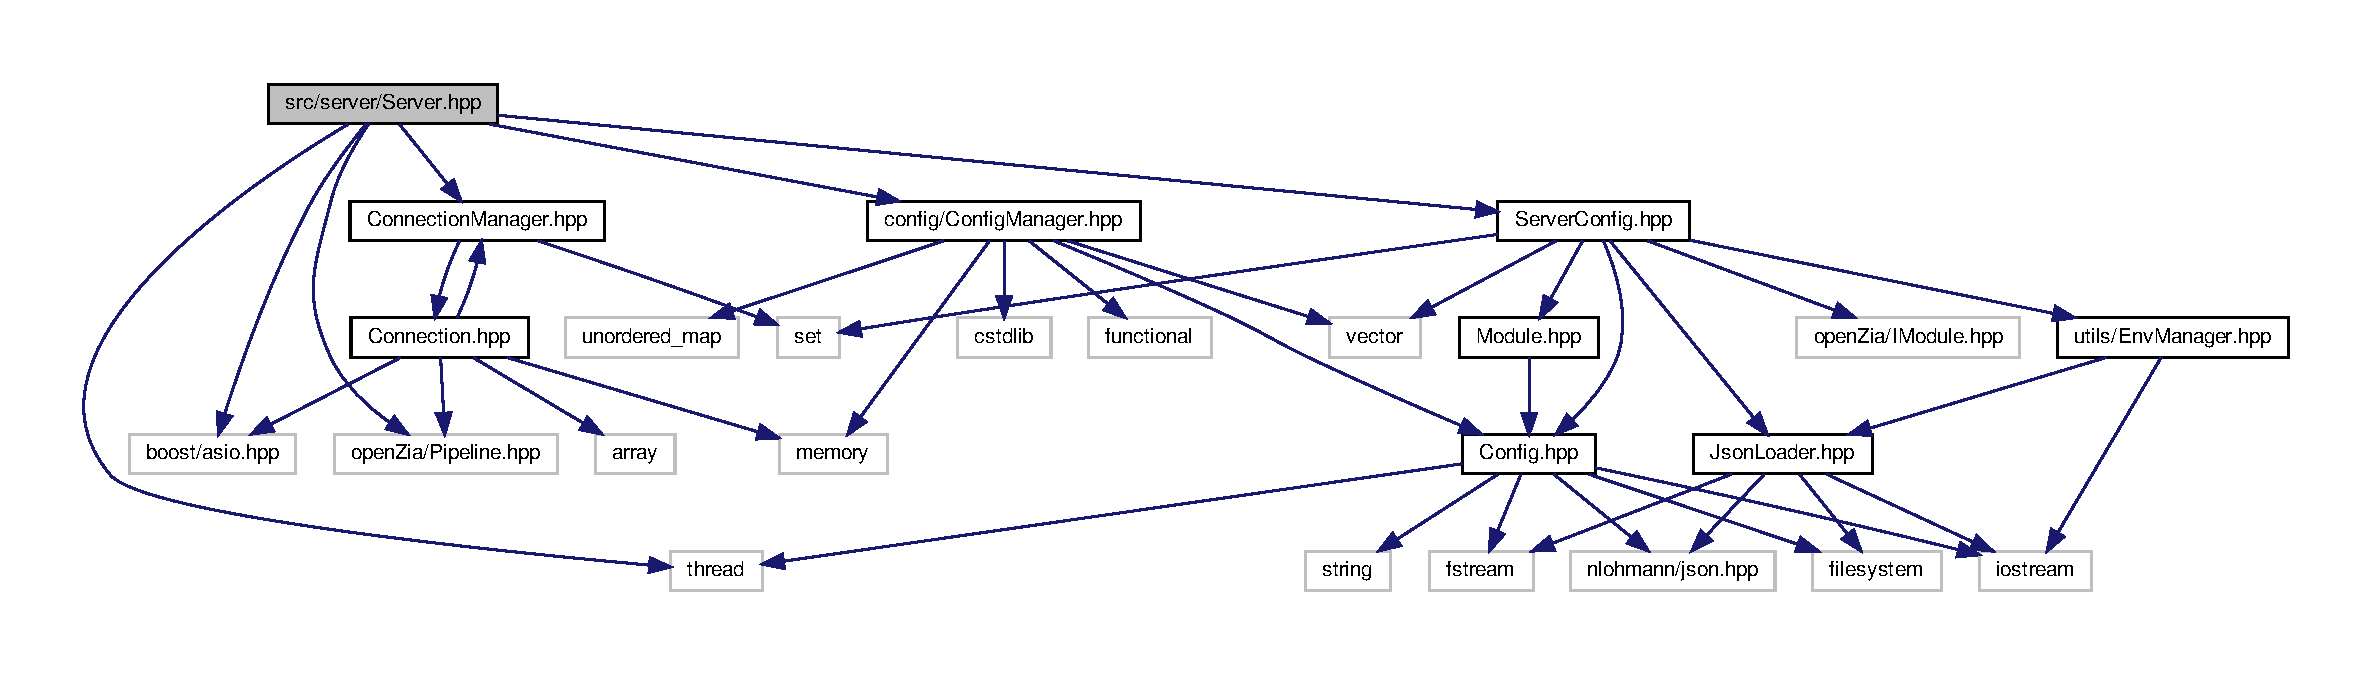
\includegraphics[width=350pt]{_server_8hpp__incl}
\end{center}
\end{figure}
This graph shows which files directly or indirectly include this file\+:\nopagebreak
\begin{figure}[H]
\begin{center}
\leavevmode
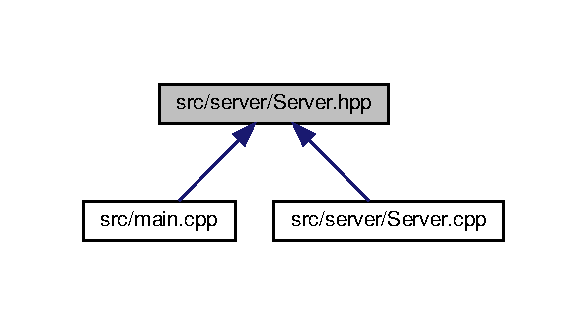
\includegraphics[width=282pt]{_server_8hpp__dep__incl}
\end{center}
\end{figure}
\subsection*{Classes}
\begin{DoxyCompactItemize}
\item 
class \hyperlink{class_zia_1_1_server}{Zia\+::\+Server}
\begin{DoxyCompactList}\small\item\em \hyperlink{class_zia_1_1_server}{Server} class to manage the server. \end{DoxyCompactList}\end{DoxyCompactItemize}
\subsection*{Namespaces}
\begin{DoxyCompactItemize}
\item 
 \hyperlink{namespace_zia}{Zia}
\end{DoxyCompactItemize}

\hypertarget{_server_config_8cpp}{}\section{src/server/\+Server\+Config.cpp File Reference}
\label{_server_config_8cpp}\index{src/server/\+Server\+Config.\+cpp@{src/server/\+Server\+Config.\+cpp}}
{\ttfamily \#include \char`\"{}Server\+Config.\+hpp\char`\"{}}\newline
Include dependency graph for Server\+Config.\+cpp\+:\nopagebreak
\begin{figure}[H]
\begin{center}
\leavevmode
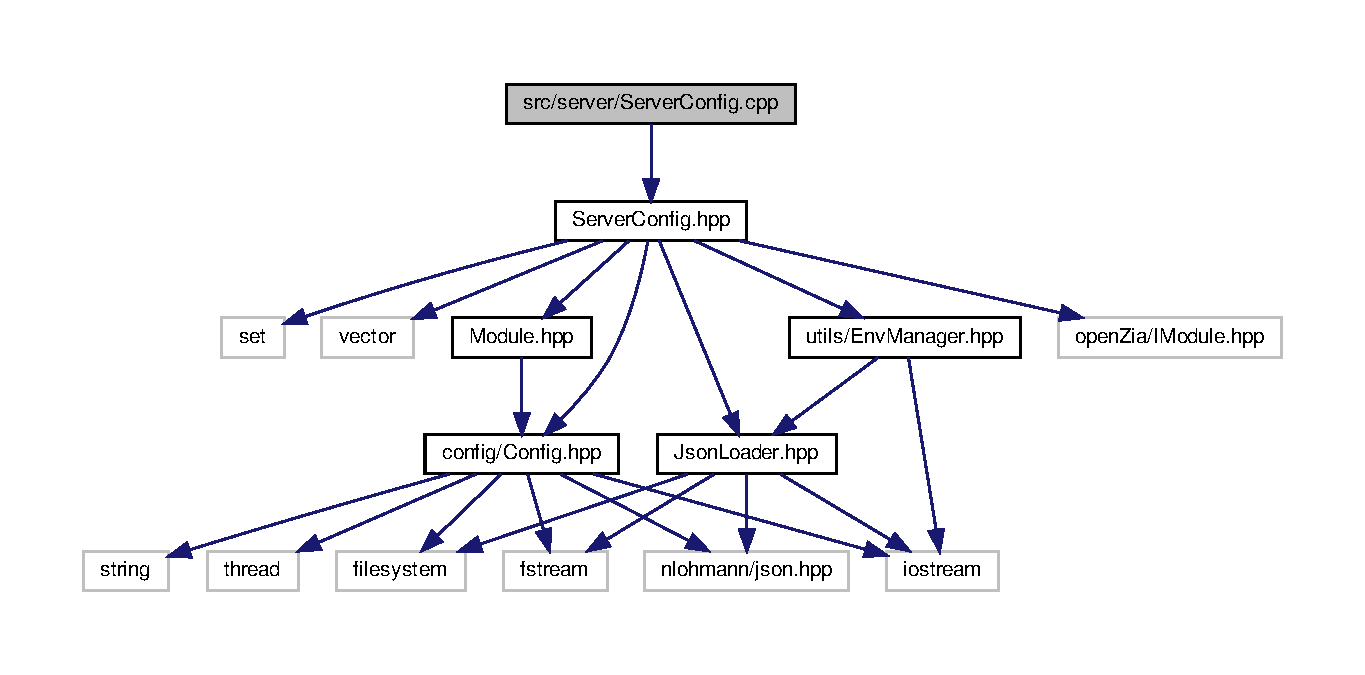
\includegraphics[width=350pt]{_server_config_8cpp__incl}
\end{center}
\end{figure}

\hypertarget{_server_config_8hpp}{}\section{src/server/\+Server\+Config.hpp File Reference}
\label{_server_config_8hpp}\index{src/server/\+Server\+Config.\+hpp@{src/server/\+Server\+Config.\+hpp}}
{\ttfamily \#include $<$set$>$}\newline
{\ttfamily \#include $<$vector$>$}\newline
{\ttfamily \#include $<$config/\+Config.\+hpp$>$}\newline
{\ttfamily \#include $<$open\+Zia/\+I\+Module.\+hpp$>$}\newline
{\ttfamily \#include $<$utils/\+Env\+Manager.\+hpp$>$}\newline
{\ttfamily \#include $<$utils/\+Json\+Loader.\+hpp$>$}\newline
{\ttfamily \#include \char`\"{}Module.\+hpp\char`\"{}}\newline
Include dependency graph for Server\+Config.\+hpp\+:\nopagebreak
\begin{figure}[H]
\begin{center}
\leavevmode
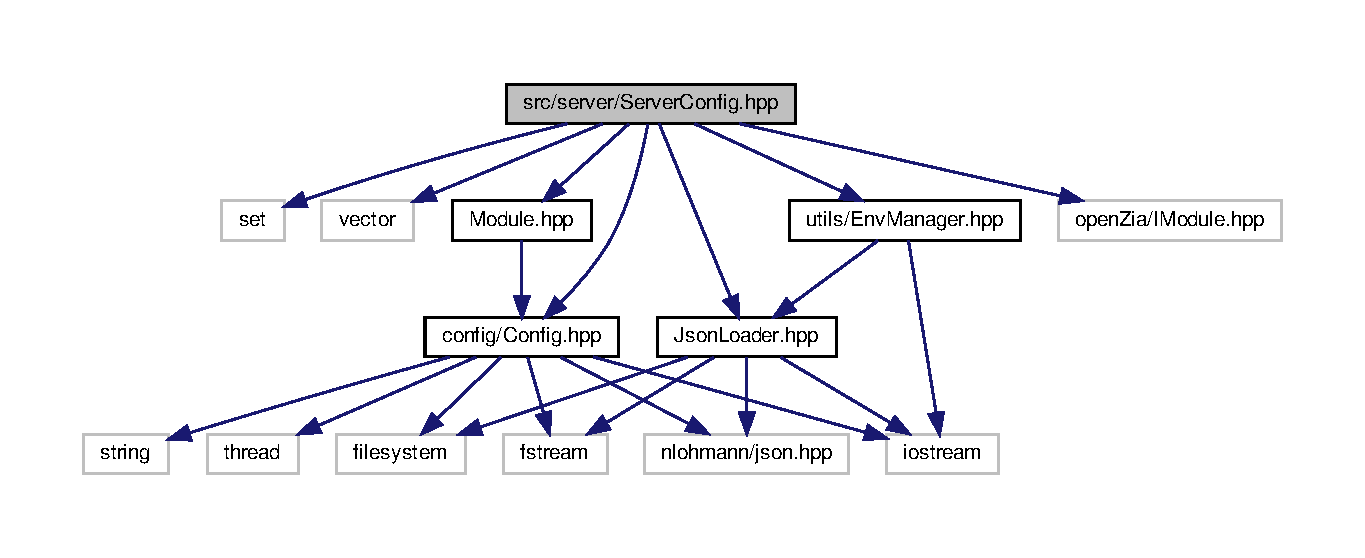
\includegraphics[width=350pt]{_server_config_8hpp__incl}
\end{center}
\end{figure}
This graph shows which files directly or indirectly include this file\+:\nopagebreak
\begin{figure}[H]
\begin{center}
\leavevmode
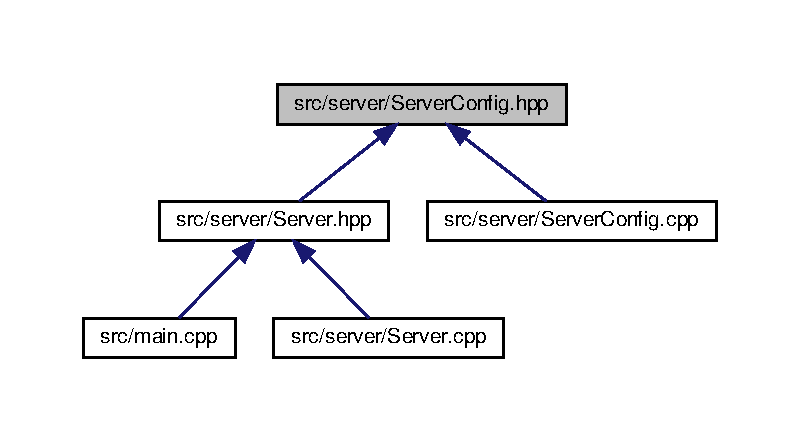
\includegraphics[width=350pt]{_server_config_8hpp__dep__incl}
\end{center}
\end{figure}
\subsection*{Classes}
\begin{DoxyCompactItemize}
\item 
class \hyperlink{class_zia_1_1_server_config}{Zia\+::\+Server\+Config}
\begin{DoxyCompactList}\small\item\em \hyperlink{class_zia_1_1_server_config}{Server\+Config} class to manage configuration files of the server. \end{DoxyCompactList}\end{DoxyCompactItemize}
\subsection*{Namespaces}
\begin{DoxyCompactItemize}
\item 
 \hyperlink{namespace_zia}{Zia}
\end{DoxyCompactItemize}
\subsection*{Typedefs}
\begin{DoxyCompactItemize}
\item 
using \hyperlink{namespace_zia_a26a1cd43d7216ed69ef26b99d8d12093}{Zia\+::\+Module\+Ptr} = std\+::shared\+\_\+ptr$<$ Module $>$
\begin{DoxyCompactList}\small\item\em \hyperlink{class_zia_1_1_module}{Module} pointer type, using shared\+\_\+ptr as backend. \end{DoxyCompactList}\item 
using \hyperlink{namespace_zia_a3076ef33a6c08b068cb8e444848ad33c}{Zia\+::\+Enabled\+List} = std\+::set$<$ Module\+Ptr $>$
\begin{DoxyCompactList}\small\item\em Set containing Module\+Ptr modules. \end{DoxyCompactList}\end{DoxyCompactItemize}
\subsection*{Variables}
\begin{DoxyCompactItemize}
\item 
const int \hyperlink{namespace_zia_a7b72c978ae2e795f74ce73291ebe3593}{Zia\+::\+Default\+Port} = 80
\begin{DoxyCompactList}\small\item\em Default H\+T\+TP port. \end{DoxyCompactList}\item 
const int \hyperlink{namespace_zia_ae53d6fd6614900bbc59b6912d6a629d4}{Zia\+::\+Default\+Port\+H\+T\+T\+PS} = 443
\begin{DoxyCompactList}\small\item\em Default H\+T\+T\+PS port. \end{DoxyCompactList}\item 
const std\+::string \hyperlink{namespace_zia_a40d4cbc794a3ff3df7017ff08173978f}{Zia\+::\+Default\+IP} = \char`\"{}127.\+0.\+0.\+1\char`\"{}
\begin{DoxyCompactList}\small\item\em Default IP address. \end{DoxyCompactList}\end{DoxyCompactItemize}

\hypertarget{_env_manager_8cpp}{}\section{src/utils/\+Env\+Manager.cpp File Reference}
\label{_env_manager_8cpp}\index{src/utils/\+Env\+Manager.\+cpp@{src/utils/\+Env\+Manager.\+cpp}}
{\ttfamily \#include \char`\"{}Env\+Manager.\+hpp\char`\"{}}\newline
Include dependency graph for Env\+Manager.\+cpp\+:\nopagebreak
\begin{figure}[H]
\begin{center}
\leavevmode
\includegraphics[width=350pt]{_env_manager_8cpp__incl}
\end{center}
\end{figure}

\hypertarget{_env_manager_8hpp}{}\section{src/utils/\+Env\+Manager.hpp File Reference}
\label{_env_manager_8hpp}\index{src/utils/\+Env\+Manager.\+hpp@{src/utils/\+Env\+Manager.\+hpp}}
{\ttfamily \#include $<$iostream$>$}\newline
{\ttfamily \#include \char`\"{}Json\+Loader.\+hpp\char`\"{}}\newline
Include dependency graph for Env\+Manager.\+hpp\+:\nopagebreak
\begin{figure}[H]
\begin{center}
\leavevmode
\includegraphics[width=350pt]{_env_manager_8hpp__incl}
\end{center}
\end{figure}
This graph shows which files directly or indirectly include this file\+:\nopagebreak
\begin{figure}[H]
\begin{center}
\leavevmode
\includegraphics[width=350pt]{_env_manager_8hpp__dep__incl}
\end{center}
\end{figure}
\subsection*{Classes}
\begin{DoxyCompactItemize}
\item 
class \hyperlink{classtls_1_1_env_manager}{tls\+::\+Env\+Manager}
\begin{DoxyCompactList}\small\item\em \hyperlink{classtls_1_1_env_manager}{Env\+Manager} class to manage environment variables. \end{DoxyCompactList}\end{DoxyCompactItemize}
\subsection*{Namespaces}
\begin{DoxyCompactItemize}
\item 
 \hyperlink{namespacetls}{tls}
\end{DoxyCompactItemize}

\hypertarget{_json_loader_8cpp}{}\section{src/utils/\+Json\+Loader.cpp File Reference}
\label{_json_loader_8cpp}\index{src/utils/\+Json\+Loader.\+cpp@{src/utils/\+Json\+Loader.\+cpp}}
{\ttfamily \#include \char`\"{}Json\+Loader.\+hpp\char`\"{}}\newline
Include dependency graph for Json\+Loader.\+cpp\+:\nopagebreak
\begin{figure}[H]
\begin{center}
\leavevmode
\includegraphics[width=350pt]{_json_loader_8cpp__incl}
\end{center}
\end{figure}

\hypertarget{_json_loader_8hpp}{}\section{src/utils/\+Json\+Loader.hpp File Reference}
\label{_json_loader_8hpp}\index{src/utils/\+Json\+Loader.\+hpp@{src/utils/\+Json\+Loader.\+hpp}}
{\ttfamily \#include $<$filesystem$>$}\newline
{\ttfamily \#include $<$fstream$>$}\newline
{\ttfamily \#include $<$iostream$>$}\newline
{\ttfamily \#include $<$nlohmann/json.\+hpp$>$}\newline
Include dependency graph for Json\+Loader.\+hpp\+:\nopagebreak
\begin{figure}[H]
\begin{center}
\leavevmode
\includegraphics[width=350pt]{_json_loader_8hpp__incl}
\end{center}
\end{figure}
This graph shows which files directly or indirectly include this file\+:\nopagebreak
\begin{figure}[H]
\begin{center}
\leavevmode
\includegraphics[width=350pt]{_json_loader_8hpp__dep__incl}
\end{center}
\end{figure}
\subsection*{Classes}
\begin{DoxyCompactItemize}
\item 
class \hyperlink{classtls_1_1_json_loader}{tls\+::\+Json\+Loader}
\begin{DoxyCompactList}\small\item\em \hyperlink{classtls_1_1_json_loader}{Json\+Loader} class to manage a json file. \end{DoxyCompactList}\end{DoxyCompactItemize}
\subsection*{Namespaces}
\begin{DoxyCompactItemize}
\item 
 \hyperlink{namespacetls}{tls}
\end{DoxyCompactItemize}
\subsection*{Typedefs}
\begin{DoxyCompactItemize}
\item 
using \hyperlink{namespacetls_a4e8d32383e204ee25990db65651ea712}{tls\+::json} = nlohmann\+::json
\begin{DoxyCompactList}\small\item\em Json library object. \end{DoxyCompactList}\end{DoxyCompactItemize}

\hypertarget{_shared_memory_8cpp}{}\section{src/utils/\+Shared\+Memory.cpp File Reference}
\label{_shared_memory_8cpp}\index{src/utils/\+Shared\+Memory.\+cpp@{src/utils/\+Shared\+Memory.\+cpp}}
{\ttfamily \#include \char`\"{}Shared\+Memory.\+hpp\char`\"{}}\newline
Include dependency graph for Shared\+Memory.\+cpp\+:\nopagebreak
\begin{figure}[H]
\begin{center}
\leavevmode
\includegraphics[width=350pt]{_shared_memory_8cpp__incl}
\end{center}
\end{figure}

\hypertarget{_shared_memory_8hpp}{}\section{src/utils/\+Shared\+Memory.hpp File Reference}
\label{_shared_memory_8hpp}\index{src/utils/\+Shared\+Memory.\+hpp@{src/utils/\+Shared\+Memory.\+hpp}}
{\ttfamily \#include $<$list$>$}\newline
{\ttfamily \#include $<$stdio.\+h$>$}\newline
{\ttfamily \#include $<$string$>$}\newline
{\ttfamily \#include $<$sys/ipc.\+h$>$}\newline
{\ttfamily \#include $<$sys/shm.\+h$>$}\newline
{\ttfamily \#include $<$sys/types.\+h$>$}\newline
Include dependency graph for Shared\+Memory.\+hpp\+:\nopagebreak
\begin{figure}[H]
\begin{center}
\leavevmode
\includegraphics[width=350pt]{_shared_memory_8hpp__incl}
\end{center}
\end{figure}
This graph shows which files directly or indirectly include this file\+:\nopagebreak
\begin{figure}[H]
\begin{center}
\leavevmode
\includegraphics[width=219pt]{_shared_memory_8hpp__dep__incl}
\end{center}
\end{figure}
\subsection*{Classes}
\begin{DoxyCompactItemize}
\item 
class \hyperlink{class_shared_memory}{Shared\+Memory}
\end{DoxyCompactItemize}

%--- End generated contents ---

% Index
\backmatter
\newpage
\phantomsection
\clearemptydoublepage
\addcontentsline{toc}{chapter}{Index}
\printindex

\end{document}
